%======================================================================
% MODULE 1: Modelling and Sensor Fusion
%
% Learning Objectives:
% After completing this module, students will be able to:
% - Represent 3D orientations using rotation matrices, Euler angles, and quaternions
% - Explain why quaternions are preferred in flight control systems
% - Model IMU sensor behavior including noise and bias
% - Design and implement complementary filters for orientation estimation
% - Derive and linearize quadrotor dynamics for control design
%======================================================================

\chapter{Coordinate Frames and 3D Transformations}

%----------------------------------------------------------------------
% FIGURE: Quadrotor with World and Body Frames
%----------------------------------------------------------------------
\begin{figure}[htbp]
\centering
\begin{tikzpicture}[scale=1.0,
    % Define 3D view angles
    x={(0.866cm,-0.25cm)},
    y={(0.866cm,0.25cm)},
    z={(0cm,0.8cm)}
]
    % Ground grid
    \fill[gray!10] (-2,-2,0) -- (4,-2,0) -- (4,4,0) -- (-2,4,0) -- cycle;
    \foreach \i in {-2,-1,...,4} {
        \draw[gray!30, thin] (\i,-2,0) -- (\i,4,0);
        \draw[gray!30, thin] (-2,\i,0) -- (4,\i,0);
    }

    % World frame {W} at origin
    \draw[xaxisstyle] (0,0,0) -- (2.5,0,0) node[below right] {$x_W$ (North)};
    \draw[yaxisstyle] (0,0,0) -- (0,2.5,0) node[below right] {$y_W$ (East)};
    \draw[zaxisstyle] (0,0,0) -- (0,0,-1.8) node[left] {$z_W$ (Down)};
    \node[below left] at (0,0,0) {$\{W\}$};

    % Quadrotor position (elevated and tilted)
    \begin{scope}[shift={(2,2,3)}, rotate around z=15, rotate around x=-12]
        % Quadrotor body (simplified X shape)
        \fill[black!20] (-0.15,-0.15,0) -- (0.15,-0.15,0) -- (0.15,0.15,0) -- (-0.15,0.15,0) -- cycle;

        % Arms
        \draw[thick, black!60] (-1.2,0,0) -- (1.2,0,0);
        \draw[thick, black!60] (0,-1.2,0) -- (0,1.2,0);

        % Motors (circles at arm ends)
        \fill[gray!50] (1.2,0,0) circle (0.2);
        \fill[gray!50] (-1.2,0,0) circle (0.2);
        \fill[gray!50] (0,1.2,0) circle (0.2);
        \fill[gray!50] (0,-1.2,0) circle (0.2);

        % Nose indicator
        \fill[red!70] (1.2,0,0.1) -- (1.4,0,0) -- (1.2,0,-0.1) -- cycle;

        % Body frame {B} (dashed)
        \draw[xaxisstyle, dashed] (0,0,0) -- (1.8,0,0) node[right] {$x_B$};
        \draw[yaxisstyle, dashed] (0,0,0) -- (0,1.8,0) node[above] {$y_B$};
        \draw[zaxisstyle, dashed] (0,0,0) -- (0,0,-1.2) node[below left] {$z_B$};
        \node[above] at (0.,0.,0) {$\{B\}$};
    \end{scope}

    % Connecting line (position vector, optional)
%    \draw[dotted, gray] (0,0,0) -- (2,2,3);

    % Annotations
    \node[annot, text width=3.5cm, align=center] at (6,1,3) {Body frame moves\\with the quadrotor};
    \node[annot, text width=3cm, align=center] at (-4,0,0) {World frame\\stays fixed};
\end{tikzpicture}
\caption{A quadrotor with two coordinate frames: the world frame $\{W\}$ fixed to the ground (NED convention), and the body frame $\{B\}$ attached to the vehicle. The body frame is tilted relative to the world frame, illustrating that transformations between frames are needed for control.}
\label{fig:world-body-frames}
\end{figure}


\section{Introduction: Why Study 3D Transformations?}

Imagine you want to fly a quadrotor from point A to point B. This seemingly simple task requires answering several fundamental questions:

\begin{itemize}
    \item \textbf{Where is the quadrotor?} We need to describe its position in 3D space.
    \item \textbf{Which way is it pointing?} We need to describe its orientation.
    \item \textbf{How do we measure these?} Sensors like accelerometers and gyroscopes give us data, but in what reference frame?
    \item \textbf{How do we command motors?} The control system must translate desired motion into motor commands, which requires understanding how the quadrotor's orientation affects its motion.
\end{itemize}

All of these questions require a precise mathematical language for describing \emph{position} and \emph{orientation} in 3D space. This chapter develops that language.

\begin{keyidea}[title=The Central Problem]
A quadrotor's sensors measure quantities in the \textbf{body frame} (attached to the quadrotor), but we want to control its motion in the \textbf{world frame} (fixed to the ground). Transforming between these frames is the mathematical heart of quadrotor control.
\end{keyidea}

\section{Coordinate Frames}

\subsection{Coordinate Conventions: ENU and NED}

Two Earth-fixed coordinate conventions are commonly used in robotics and aerospace:
\emph{ENU (East--North--Up)}\index{ENU (East-North-Up)} and \emph{NED (North--East--Down)}\index{NED (North-East-Down)}. 
Both define Cartesian coordinate frames attached to the local tangent plane of the Earth, and both are \emph{right-handed}.

In the \textbf{ENU} convention, the coordinate axes are defined as
\[
x \text{ (East)}, \quad y \text{ (North)}, \quad z \text{ (Up)} .
\]
ENU is widely used in robotics, computer vision, and simulation environments, as it aligns with standard Cartesian geometry and is intuitive for visualization, mapping, and perception tasks.

In the \textbf{NED} convention, the coordinate axes are defined as
\[
x \text{ (North)}, \quad y \text{ (East)}, \quad z \text{ (Down)} .
\]
NED is the dominant convention in aerospace and navigation and is commonly used for aircraft and quadrotor modeling, inertial navigation systems, and flight-control software.

\paragraph{Right-handed coordinate frames}
Let \(\{\mathbf{e}_x, \mathbf{e}_y, \mathbf{e}_z\}\) denote the unit basis vectors of a coordinate frame.  
The frame is said to be \emph{right-handed} if
\[
\mathbf{e}_x \times \mathbf{e}_y = \mathbf{e}_z ,
\]
where \(\times\) denotes the vector cross product. Equivalently, the ordered basis has a positive orientation, i.e.,
\[
\det\!\begin{bmatrix}
\mathbf{e}_x & \mathbf{e}_y & \mathbf{e}_z
\end{bmatrix} = +1 .
\]

This property defines the \textbf{right-hand rule}: if the index finger of the right hand points along the positive \(x\)-axis and the middle finger along the positive \(y\)-axis, the thumb points in the positive \(z\)-direction. This convention ensures consistent definitions of cross products, angular velocities, torques, and rotation directions.

Both ENU and NED satisfy this relation, even though their axes point in different physical directions (e.g., up versus down). What matters is the ordering and orientation of the axes, not their semantic labels.

\paragraph{Motivation for NED in this course}
This course adopts the NED convention because the focus is on quadrotors. NED is standard in aerospace literature and flight-control implementations, and it allows gravity to be represented as a positive acceleration along the \(z\)-axis. This simplifies the equations of motion and control design and ensures direct consistency with GNSS/IMU models and widely used autopilot frameworks.


\subsection{What is a Coordinate Frame?}

\begin{definition}[Coordinate Frame]
\index{coordinate frame}
A \textbf{coordinate frame}\index{coordinate frame|textbf} is a set of three mutually perpendicular unit vectors (axes) with a defined origin. We denote frames with curly braces: $\{W\}$, $\{B\}$, etc.
\end{definition}

\textbf{Intuition}: A coordinate frame is like a ruler system attached to an object. When you describe a point as being ``2 meters to the right,'' you're implicitly using a coordinate frame---your ``right'' defines one axis, and you're measuring distance along it.

\subsection{Why Do We Need Multiple Frames?}

Consider measuring the position of your coffee cup:
\begin{itemize}
    \item Relative to your desk: ``30 cm from the left edge, 20 cm from the front''
    \item Relative to the room: ``2 m from the north wall, 3 m from the east wall''
    \item Relative to the Earth: latitude, longitude, altitude
\end{itemize}

These are all valid descriptions of the \emph{same} position, just in different coordinate frames. For quadrotors, we primarily use two frames:

\subsection{World Frame (Inertial Frame) $\{W\}$}
\index{world frame}\index{inertial frame|see{world frame}}

The world frame\index{world frame|textbf} is fixed to the Earth and serves as our absolute reference for describing where we want the quadrotor to go.

\begin{notebox}[title=Assumption: Earth as Inertial Frame]
We assume the Earth is an \textbf{inertial frame}---not rotating or accelerating. This is valid for:
\begin{itemize}
    \item Flight durations of minutes (Earth's rotation is negligible)
    \item Altitudes below ~10 km (Earth's curvature is negligible)
    \item Non-polar regions (Coriolis effects are small)
\end{itemize}
For intercontinental flights or spacecraft, this assumption breaks down.
\end{notebox}

Two conventions are commonly used:

%----------------------------------------------------------------------
% FIGURE: NED vs ENU Coordinate Conventions
%----------------------------------------------------------------------
\begin{figure}[htbp]
\centering
\begin{tikzpicture}[scale=1.0,
    % Same 3D view as quadrotor figure for consistency
    x={(0.866cm,-0.25cm)},
    y={(0.866cm,0.25cm)},
    z={(0cm,0.8cm)}
]
    % === NED Frame (Left) ===
    \begin{scope}[shift={(-4,0)}]
        % Axes matching quadrotor figure convention
        \draw[-{Stealth}, thick, red] (0,0,0) -- (2,0,0) node[right, font=\small] {$x$ (N)};
        \draw[-{Stealth}, thick, green!70!black] (0,0,0) -- (0,2,0) node[right, font=\small] {$y$ (E)};
        \draw[-{Stealth}, thick, blue] (0,0,0) -- (0,0,-2) node[left, font=\small] {$z$ (D)};

        % Origin
        \fill (0,0,0) circle (2pt);

        % Title below axes
        \node[font=\bfseries\large] at (1,-2.5) {NED};
        \node[font=\small] at (1,-3.2) {North-East-Down};
    \end{scope}

    % === Gravity vector (centered between frames) ===
    \draw[-{Stealth}, very thick, orange] (0,0,1) -- (0,0,-1.5)
        node[left, font=\small, pos=0.5] {$\mathbf{g}$};

    % === ENU Frame (Right) ===
    \begin{scope}[shift={(4,0)}]
        % Axes
        \draw[-{Stealth}, thick, red] (0,0,0) -- (2,0,0) node[right, font=\small] {$x$ (E)};
        \draw[-{Stealth}, thick, green!70!black] (0,0,0) -- (0,2,0) node[right, font=\small] {$y$ (N)};
        \draw[-{Stealth}, thick, blue] (0,0,0) -- (0,0,2) node[left, font=\small] {$z$ (U)};

        % Origin
        \fill (0,0,0) circle (2pt);

        % Title below axes
        \node[font=\bfseries\large] at (1,-2.5) {ENU};
        \node[font=\small] at (1,-3.2) {East-North-Up};
    \end{scope}
\end{tikzpicture}
\caption{Comparison of NED (North-East-Down) and ENU (East-North-Up) coordinate conventions. In NED, gravity aligns with $+z$; in ENU, gravity aligns with $-z$. The choice affects sign conventions throughout control algorithms.}
\label{fig:ned-enu-conventions}
\end{figure}
%----------------------------------------------------------------------

\begin{center}
\begin{tabular}{lccl}
\toprule
\textbf{Convention} & \textbf{Axes} & \textbf{$z$-axis} & \textbf{Common Use} \\
\midrule
NED & North, East, Down & Points into Earth & Aviation\\
ENU & East, North, Up & Points toward sky & Robotics\\
\bottomrule
\end{tabular}
\end{center}

\begin{warningbox}[title=Convention Matters!]
The choice between NED and ENU affects:
\begin{itemize}
    \item Sign of gravity ($+g$ in NED, $-g$ in ENU)
    \item Sign of altitude (positive down in NED, positive up in ENU)
    \item Direction of positive yaw rotation
\end{itemize}
\textbf{This course uses NED unless otherwise stated.} When using external libraries or data, always verify the convention first!
\end{warningbox}

\subsection{Body Frame $\{B\}$}
\index{body frame}

The body frame\index{body frame|textbf} is rigidly attached to the quadrotor and moves with it. This is the natural frame for:
\begin{itemize}
    \item Sensor measurements (IMU measures acceleration/rotation in body frame)
    \item Thrust direction (motors push ``down'' in body frame)
    \item Aerodynamic forces (drag depends on velocity in body frame)
\end{itemize}

%----------------------------------------------------------------------
% FIGURE: Quadrotor Body Frame Definition
%----------------------------------------------------------------------
\begin{figure}[htbp]
\centering
\begin{tikzpicture}[scale=0.85]
    % === Top-down view (Left panel) ===
    \begin{scope}[shift={(-5,0)}]
        % Arms (+ configuration)
        \draw[very thick, black!60] (-2,0) -- (2,0);
        \draw[very thick, black!60] (0,-2) -- (0,2);

        % Central body
        \fill[black!30] (-0.3,-0.3) rectangle (0.3,0.3);

        % Motors
        \node[motor] (M1) at (2,0) {};
        \node[motor] (M2) at (0,-2) {};
        \node[motor] (M3) at (-2,0) {};
        \node[motor] (M4) at (0,2) {};

        % Motor labels
        \node[font=\footnotesize, above right] at (M1.north east) {M1};
        \node[font=\footnotesize, below right] at (M2.south east) {M2};
        \node[font=\footnotesize, above left] at (M3.north west) {M3};
        \node[font=\footnotesize, above left] at (M4.north west) {M4};

        % Nose indicator
        \fill[red!70] (2.3,0.15) -- (2.6,0) -- (2.3,-0.15) -- cycle;

        % Body frame axes
        \draw[xaxisstyle] (0,0) -- (3,0) node[right] {$x_B$ (forward)};
        \draw[yaxisstyle] (0,0) -- (0,-3) node[below] {$y_B$ (right)};
        \fill[black] (0,0) circle (0.08) node[above left, font=\footnotesize] {COG};

        % View label
        \node[font=\bfseries\small] at (0,3) {Top View};
    \end{scope}

    % === Side view (Right panel) ===
    \begin{scope}[shift={(4,0)}]
        % Arm (side view - just a line)
        \draw[very thick, black!60] (-2,0) -- (2,0);

        % Central body
        \fill[black!30] (-0.3,-0.15) rectangle (0.3,0.15);

        % Motors (front and back visible)
        \draw[thick, black!60, fill=gray!30] (2,0) ellipse (0.4 and 0.15);
        \draw[thick, black!60, fill=gray!30] (-2,0) ellipse (0.4 and 0.15);

        % Landing gear
        \draw[thick, black!50] (-0.8,0) -- (-0.8,-0.8) -- (-1,-0.8);
        \draw[thick, black!50] (0.8,0) -- (0.8,-0.8) -- (1,-0.8);
        \draw[thick, black!50] (-1,-0.8) -- (1,-0.8);

        % Nose indicator
        \fill[red!70] (2.3,0.1) -- (2.5,0) -- (2.3,-0.1) -- cycle;

        % Body frame axes
        \draw[xaxisstyle] (0,0) -- (3,0) node[right] {$x_B$};
        \draw[zaxisstyle] (0,0) -- (0,-2) node[below] {$z_B$ (down)};
        \fill[black] (0,0) circle (0.08) node[above left, font=\footnotesize] {COG};

        % View label
        \node[font=\bfseries\small] at (0,1.5) {Side View};

        % "Pilot perspective" annotation
        \draw[<-, gray, thin] (0.5,0.5) -- (1.5,1)
            node[right, font=\scriptsize, text width=2cm] {Sitting inside: forward, right, down};
    \end{scope}
\end{tikzpicture}
\caption{Body frame definition for a quadrotor in + configuration. Left: top-down view showing $x_B$ (forward) and $y_B$ (right) axes. Right: side view showing $x_B$ and $z_B$ (down) axes. The origin is at the center of gravity (COG).}
\label{fig:body-frame-definition}
\end{figure}
%----------------------------------------------------------------------

\textbf{Standard definition} (for NED world frame):
\begin{itemize}
    \item \textbf{Origin}: Center of gravity (COG)
    \item \textbf{$x_B$}: Points forward (``nose'' direction)
    \item \textbf{$y_B$}: Points right (starboard)
    \item \textbf{$z_B$}: Points down (toward landing gear)
\end{itemize}

\textbf{Intuition}: Imagine sitting inside the quadrotor. The body frame axes are your ``forward,'' ``right,'' and ``down.''

\section{Describing Orientation: The Rotation Matrix}
\index{rotation matrix}

\subsection{The Problem}

We need to answer: ``How is the body frame oriented relative to the world frame?''

Equivalently: ``If I know a vector's coordinates in the body frame, what are its coordinates in the world frame?''

\subsection{Building Intuition in 2D}

Before tackling 3D, let's understand rotations in 2D, where the math is simpler.

Consider a vector $\mathbf{v}$ that has coordinates $(v_x, v_y)$ in a frame $\{A\}$. If frame $\{B\}$ is rotated by angle $\theta$ counter-clockwise relative to $\{A\}$, what are the coordinates of $\mathbf{v}$ in frame $\{A\}$ if we know them in frame $\{B\}$?

%----------------------------------------------------------------------
% FIGURE: 2D Rotation Between Frames
%----------------------------------------------------------------------
\begin{figure}[htbp]
\centering
\begin{tikzpicture}[scale=1.1]
    % Define angle
    \pgfmathsetmacro{\angle}{35}

    % Frame {A} axes (solid, black)
    \draw[axis, frameA] (0,0) -- (3.5,0) node[right] {$x_A$};
    \draw[axis, frameA] (0,0) -- (0,3.5) node[above] {$y_A$};
    \node[below left] at (0,0) {$O$};

    % Frame {B} axes (dashed, gray) rotated by theta
    \draw[dashedaxis, frameB] (0,0) -- ({3.2*cos(\angle)},{3.2*sin(\angle)}) node[right] {$x_B$};
    \draw[dashedaxis, frameB] (0,0) -- ({-3.2*sin(\angle)},{3.2*cos(\angle)}) node[above] {$y_B$};

    % Angle arc and label
    \draw[thick, blue!70] (1.2,0) arc (0:\angle:1.2);
    \node[blue!70] at ({1.5*cos(\angle/2)},{1.5*sin(\angle/2)}) {$\theta$};

    % Vector v
    \pgfmathsetmacro{\vx}{2.5}
    \pgfmathsetmacro{\vy}{2.0}
    \draw[vec, line width=1.5pt] (0,0) -- (\vx,\vy) node[above right] {$\mathbf{v}$};
    \fill[vectorcolor] (\vx,\vy) circle (0.06);

    % Projections onto frame A (dotted)
    \draw[dotted, thick, xaxis] (\vx,\vy) -- (\vx,0) node[below, font=\small] {$v_x^A$};
    \draw[dotted, thick, yaxis] (\vx,\vy) -- (0,\vy) node[left, font=\small] {$v_y^A$};

    % Projections onto frame B (dotted, lighter)
    \pgfmathsetmacro{\vxB}{\vx*cos(\angle)+\vy*sin(\angle)} % v dot x_B_hat
    \pgfmathsetmacro{\vyB}{-\vx*sin(\angle)+\vy*cos(\angle)} % v dot y_B_hat
    \coordinate (vBx) at ({(\vxB)*cos(\angle)},{(\vxB)*sin(\angle)});
    \coordinate (vBy) at ({-(\vyB)*sin(\angle)},{(\vyB)*cos(\angle)});
    \draw[dotted, thick, gray!60] (\vx,\vy) -- (vBx);
    \draw[dotted, thick, gray!60] (\vx,\vy) -- (vBy);
    \node[font=\small, gray!70] at ($(vBx)+(0.3,-0.3)$) {$v_x^B$};
    \node[font=\small, gray!70] at ($(vBy)+(-0.4,0.2)$) {$v_y^B$};

    % Annotation: column interpretation
    \node[text width=4.5cm, font=\small, align=left] at (5.5,2.5) {
        \textbf{Rotation matrix columns:}\\[2pt]
        1st column: $\hat{x}_B$ in $\{A\}$\\
        $= [\cos\theta, \sin\theta]^T$\\[4pt]
        2nd column: $\hat{y}_B$ in $\{A\}$\\
        $= [-\sin\theta, \cos\theta]^T$
    };

    % Annotation box
    \node[draw, rounded corners, fill=blue!5, text width=3.5cm, font=\small, align=center]
        at (5.5,-0.3) {Same vector $\mathbf{v}$,\\different coordinates\\in each frame};
\end{tikzpicture}
\caption{A vector $\mathbf{v}$ expressed in two coordinate frames. Frame $\{B\}$ is rotated by angle $\theta$ relative to frame $\{A\}$. The rotation matrix columns tell us where the rotated frame's unit vectors point.}
\label{fig:2d-rotation-frames}
\end{figure}
%----------------------------------------------------------------------

\begin{equation}
\begin{bmatrix} v_x^A \\ v_y^A \end{bmatrix} =
\underbrace{\begin{bmatrix} \cos\theta & -\sin\theta \\ \sin\theta & \cos\theta \end{bmatrix}}_{R(\theta)}
\begin{bmatrix} v_x^B \\ v_y^B \end{bmatrix}
\end{equation}

\textbf{Intuition}: The rotation matrix $R(\theta)$ tells us where the $x$ and $y$ axes of frame $\{B\}$ point when expressed in frame $\{A\}$:
\begin{itemize}
    \item First column: where $\hat{x}_B$ points in $\{A\}$
    \item Second column: where $\hat{y}_B$ points in $\{A\}$
\end{itemize}

\begin{keyidea}[title=Properties of Rotation Matrices]
Rotation matrices have special structure:
\begin{itemize}
    \item \textbf{Orthogonal}: $R^T R = I$, so $R^{-1} = R^T$ (inverse is just transpose)
    \item \textbf{Unit determinant}: $\det(R) = +1$ (preserves volume and handedness)
    \item \textbf{Columns are orthonormal}: Each column is a unit vector, and columns are perpendicular
\end{itemize}
These properties reflect the physical fact that rotation preserves lengths, angles and orientation.
\end{keyidea}

\begin{definition}[Rotation]
A \emph{rotation} in $\mathbb{R}^n$, with $n \ge 2$, is a linear transformation
$R:\mathbb{R}^n \rightarrow \mathbb{R}^n$ that preserves lengths, angles, and
orientation. Equivalently, for all vectors $x,y \in \mathbb{R}^n$,
\begin{equation}
(Rx)\cdot(Ry) = x \cdot y ,
\end{equation}
and positively oriented coordinate frames remain positively oriented after the
transformation. 
\end{definition}


\paragraph{Property 1: Orthogonality.}
From inner-product preservation, remember that $x \cdot y = x^\top y$ and $(Ax)^\top=x^\top A^\top$, we have
\[
(Rx)\cdot(Ry) = (Rx)^\top R y = x^\top R^\top R y = x^\top y
\quad \forall x,y .
\]
This implies
\begin{equation}
R^\top R = I .
\end{equation}
Hence, the columns (and rows) of $R$ form an orthonormal basis, and $R$ is an orthogonal matrix.

\paragraph{Property 2: Inverse equals transpose.}
Since $R^\top R = I$, the inverse of $R$ exists and is given by
\begin{equation}
R^{-1} = R^\top .
\end{equation}
Geometrically, this corresponds to the fact that applying a rotation and then its reverse restores the original vectors.

\paragraph{Property 3: Determinant equals $+1$.}
Orthogonality implies $\lvert \det(R) \rvert = 1$, which expresses volume preservation.
Because a rotation preserves orientation (right-handedness), reflections are excluded, and therefore
\begin{equation}
\det(R) = +1.
\end{equation}

\begin{definition}[Special Orthogonal group]
A rotation matrix is therefore an orthogonal matrix with determinant $+1$. In $n$ dimensions, the set of all such matrices forms the group $SO(n)$, known as the \emph{Special Orthogonal group} in $n \geq 2$ dimensions, i.e.,
\[
SO(n) = \{ R \in \mathbb{R}^{n\times n} \mid R^\top R = I,\ \det(R)=+1 \}.
\]
\end{definition}

In our context, we are primarily concerned with rotations in two and three
dimensions. The difference between $SO(2)$ and $SO(3)$ is primarily one of dimensionality and
degrees of freedom. A general $3\times 3$ matrix has $9$ independent elements, but a
3D rotation has only $3$ degrees of freedom. This reduction follows from the
orthogonality condition $R^\top R = I$, which requires the three column vectors of
$R$ to form an orthonormal basis. Concretely, this imposes three constraints that each
column has unit length and three additional constraints that distinct columns are
mutually orthogonal, yielding $6$ independent scalar constraints in total. Subtracting
these from the original $9$ free parameters leaves $9-6=3$ degrees of freedom. The
determinant condition $\det(R)=+1$ does not further reduce this number; it merely
excludes reflections.

Despite this difference, rotations in 2D and 3D share the same fundamental properties:
they preserve lengths, angles, and orientation, satisfy $R^\top R = I$,
$R^{-1}=R^\top$, and compose by matrix multiplication. The key distinction is that a
2D rotation acts in a plane and is fully specified by a single angle (one degree of
freedom), whereas a 3D rotation specifies an orientation in space and requires three
degrees of freedom. This also affects rotation order: in 2D, all rotations are about
the same axis and therefore commute, while in 3D rotations about different axes
generally do not commute, making the order of rotations significant.
\subsection{3D Elementary Rotations}

In 3D, we can rotate about any of the three coordinate axes. The rotation matrices are:

%----------------------------------------------------------------------
% FIGURE: Elementary 3D Rotations (Roll, Pitch, Yaw)
%----------------------------------------------------------------------
\begin{figure}[htbp]
\centering
\begin{tikzpicture}[scale=0.75]
    % === Panel 1: Roll (about x-axis) ===
    \begin{scope}[shift={(-5.5,0)},
        x={(0.7cm,-0.4cm)}, y={(0.7cm,0.4cm)}, z={(0cm,0.9cm)}]

        % Axes
        \draw[xaxisstyle, line width=1.5pt] (0,0,0) -- (2.5,0,0) node[right] {$x$};
        \draw[yaxisstyle] (0,0,0) -- (0,2,0) node[above right] {$y$};
        \draw[zaxisstyle] (0,0,0) -- (0,0,2) node[above] {$z$};

        % Rotation arc around x-axis
        \draw[thick, xaxis, -{Stealth}] (0,0,1.3) arc (90:0:1.3) node[pos=0.5, right] {$\phi$};

        % Quadrotor (tilted - roll)
        \begin{scope}[rotate around x=25]
            \draw[thick, gray] (-0.8,0,1.8) -- (0.8,0,1.8);
            \draw[thick, gray] (0,-0.8,1.8) -- (0,0.8,1.8);
            \fill[gray!40] (0.8,0,1.8) circle (0.15);
            \fill[gray!40] (-0.8,0,1.8) circle (0.15);
            \fill[gray!40] (0,0.8,1.8) circle (0.15);
            \fill[gray!40] (0,-0.8,1.8) circle (0.15);
        \end{scope}

        % Label
        \node[font=\bfseries\small, text width=2.5cm, align=center] at (0,-1.5,0)
            {Roll ($\phi$)\\about $x$-axis};
    \end{scope}

    % === Panel 2: Pitch (about y-axis) ===
    \begin{scope}[shift={(0,0)},
        x={(0.7cm,-0.4cm)}, y={(0.7cm,0.4cm)}, z={(0cm,0.9cm)}]

        % Axes
        \draw[xaxisstyle] (0,0,0) -- (2,0,0) node[right] {$x$};
        \draw[yaxisstyle, line width=1.5pt] (0,0,0) -- (0,2.5,0) node[above right] {$y$};
        \draw[zaxisstyle] (0,0,0) -- (0,0,2) node[above] {$z$};

        % Rotation arc around y-axis
        \draw[thick, yaxis, -{Stealth}] (1.3,0,0) arc (0:90:1.3) node[pos=0.5, above left] {$\theta$};

        % Quadrotor (tilted - pitch)
        \begin{scope}[rotate around y=-20]
            \draw[thick, gray] (-0.8,0,1.8) -- (0.8,0,1.8);
            \draw[thick, gray] (0,-0.8,1.8) -- (0,0.8,1.8);
            \fill[gray!40] (0.8,0,1.8) circle (0.15);
            \fill[gray!40] (-0.8,0,1.8) circle (0.15);
            \fill[gray!40] (0,0.8,1.8) circle (0.15);
            \fill[gray!40] (0,-0.8,1.8) circle (0.15);
        \end{scope}

        % Label
        \node[font=\bfseries\small, text width=2.5cm, align=center] at (0,-1.5,0)
            {Pitch ($\theta$)\\about $y$-axis};
    \end{scope}

    % === Panel 3: Yaw (about z-axis) ===
    \begin{scope}[shift={(5.5,0)},
        x={(0.7cm,-0.4cm)}, y={(0.7cm,0.4cm)}, z={(0cm,0.9cm)}]

        % Axes
        \draw[xaxisstyle] (0,0,0) -- (2,0,0) node[right] {$x$};
        \draw[yaxisstyle] (0,0,0) -- (0,2,0) node[above right] {$y$};
        \draw[zaxisstyle, line width=1.5pt] (0,0,0) -- (0,0,2.5) node[above] {$z$};

        % Rotation arc around z-axis (in xy plane)
        \draw[thick, zaxis, -{Stealth}] (1.3,0,0) arc (0:70:1.3);
        \node[zaxis] at (0.6,1.1,0) {$\psi$};

        % Quadrotor (rotated - yaw)
        \begin{scope}[rotate around z=25]
            \draw[thick, gray] (-0.8,0,1.8) -- (0.8,0,1.8);
            \draw[thick, gray] (0,-0.8,1.8) -- (0,0.8,1.8);
            \fill[gray!40] (0.8,0,1.8) circle (0.15);
            \fill[gray!40] (-0.8,0,1.8) circle (0.15);
            \fill[gray!40] (0,0.8,1.8) circle (0.15);
            \fill[gray!40] (0,-0.8,1.8) circle (0.15);
            % Nose marker
            \fill[red!70] (0.9,0,1.8) -- (1.05,0,1.8) -- (0.9,0.1,1.8) -- cycle;
        \end{scope}

        % Label
        \node[font=\bfseries\small, text width=2.5cm, align=center] at (0,-1.5,0)
            {Yaw ($\psi$)\\about $z$-axis};
    \end{scope}

    % Right-hand rule reminder at bottom
    \node[draw, rounded corners, fill=yellow!10, font=\small, text width=10cm, align=center]
        at (0,-3.5) {
        \textbf{Right-hand rule:} Point thumb along positive axis direction;
        fingers curl in positive rotation direction.
    };
\end{tikzpicture}
\caption{Elementary rotations about the three principal axes. Roll ($\phi$) rotates about the $x$-axis, pitch ($\theta$) about the $y$-axis, and yaw ($\psi$) about the $z$-axis. The highlighted axis in each panel is the rotation axis.}
\label{fig:elementary-rotations}
\end{figure}
%----------------------------------------------------------------------

\textbf{Rotation about $x$-axis by angle $\phi$} (roll):
\begin{equation}
R_x(\phi) = \begin{bmatrix}
1 & 0 & 0 \\
0 & \cos\phi & -\sin\phi \\
0 & \sin\phi & \cos\phi
\end{bmatrix}
\end{equation}

\textbf{Intuition}: The $x$-axis stays fixed; the $y$ and $z$ axes rotate in the $yz$-plane.

\textbf{Rotation about $y$-axis by angle $\theta$} (pitch):
\begin{equation}
R_y(\theta) = \begin{bmatrix}
\cos\theta & 0 & \sin\theta \\
0 & 1 & 0 \\
-\sin\theta & 0 & \cos\theta
\end{bmatrix}
\end{equation}

\textbf{Rotation about $z$-axis by angle $\psi$} (yaw):
\begin{equation}
R_z(\psi) = \begin{bmatrix}
\cos\psi & -\sin\psi & 0 \\
\sin\psi & \cos\psi & 0 \\
0 & 0 & 1
\end{bmatrix}
\end{equation}

\begin{notebox}[title=Notation: Euler Angles]
The angles $(\phi, \theta, \psi)$ have standard names in aerospace:
\begin{itemize}
    \item $\phi$ (phi): \textbf{Roll} --- rotation about the forward ($x$) axis
    \item $\theta$ (theta): \textbf{Pitch} --- rotation about the lateral ($y$) axis
    \item $\psi$ (psi): \textbf{Yaw} --- rotation about the vertical ($z$) axis
\end{itemize}
Positive directions follow the \textbf{right-hand rule}: thumb along axis, fingers curl in positive rotation direction.
\end{notebox}

\subsection{The Critical Difference from 2D: Order Matters!}

\begin{warningbox}[title=Non-Commutativity of 3D Rotations]
In 2D, the order of rotations doesn't matter: rotating 30° then 45° gives the same result as 45° then 30°.

\textbf{In 3D, order matters!}
\[
R_x(\alpha) R_y(\beta) \neq R_y(\beta) R_x(\alpha)
\]
This is perhaps the most important conceptual difference between 2D and 3D geometry.
\end{warningbox}

%----------------------------------------------------------------------
% FIGURE: Rotation Order Matters (Non-Commutativity)
%----------------------------------------------------------------------
\begin{figure}[htbp]
\centering
\begin{tikzpicture}[scale=0.65,
    book/.style={thick},
    bookcover/.style={fill=blue!30, draw=blue!60},
    bookspine/.style={fill=blue!50, draw=blue!70},
    bookpages/.style={fill=gray!10, draw=gray!50}
]
    % Helper for drawing a 3D book with orientation
    % Row 1: Pitch then Yaw
    \node[font=\bfseries] at (-6, 2.5) {Sequence A:};

    % A1: Start - book flat
    \begin{scope}[shift={(-5,0)}]
        \fill[bookcover] (-0.8,-0.5) rectangle (0.8,0.5);
        \fill[bookspine] (-0.8,-0.5) -- (-0.8,0.5) -- (-0.9,0.6) -- (-0.9,-0.4) -- cycle;
        \fill[bookpages] (0.8,-0.5) -- (0.8,0.5) -- (0.9,0.6) -- (0.9,-0.4) -- cycle;
        \node[font=\scriptsize] at (0,0) {Cover};
        \node[below, font=\small] at (0,-1) {Start};
    \end{scope}

    \draw[-{Stealth}, thick] (-3.5,0) -- (-2.5,0) node[midway, above, font=\scriptsize] {Pitch 90°};

    % A2: After pitch - cover faces forward
    \begin{scope}[shift={(-1,0)}]
        \fill[bookpages] (-0.8,-0.5) rectangle (0.8,0.5);
        \fill[bookspine] (-0.8,-0.5) -- (-0.8,0.5) -- (-0.9,0.4) -- (-0.9,-0.6) -- cycle;
        \fill[bookcover] (-0.8,-0.5) -- (0.8,-0.5) -- (0.9,-0.6) -- (-0.9,-0.6) -- cycle;
        \node[font=\scriptsize, rotate=-10] at (0,-0.7) {Cover};
    \end{scope}

    \draw[-{Stealth}, thick] (0.5,0) -- (1.5,0) node[midway, above, font=\scriptsize] {Yaw 90°};

    % A3: Final A - after yaw
    \begin{scope}[shift={(3,0)}]
        \fill[bookpages] (-0.5,-0.8) rectangle (0.5,0.8);
        \fill[bookcover] (0.5,-0.8) -- (0.5,0.8) -- (0.6,0.7) -- (0.6,-0.9) -- cycle;
        \fill[bookspine] (-0.5,0.8) -- (0.5,0.8) -- (0.6,0.7) -- (-0.4,0.7) -- cycle;
        \node[font=\scriptsize, rotate=90] at (0.7,0) {Cover};
        \node[below, font=\small\bfseries, red!70!black] at (0,-1.2) {Final A};
    \end{scope}

    % Row 2: Yaw then Pitch
    \node[font=\bfseries] at (-6, -2.5) {Sequence B:};

    % B1: Start - book flat (same as A1)
    \begin{scope}[shift={(-5,-4)}]
        \fill[bookcover] (-0.8,-0.5) rectangle (0.8,0.5);
        \fill[bookspine] (-0.8,-0.5) -- (-0.8,0.5) -- (-0.9,0.6) -- (-0.9,-0.4) -- cycle;
        \fill[bookpages] (0.8,-0.5) -- (0.8,0.5) -- (0.9,0.6) -- (0.9,-0.4) -- cycle;
        \node[font=\scriptsize] at (0,0) {Cover};
        \node[below, font=\small] at (0,-1) {Start};
    \end{scope}

    \draw[-{Stealth}, thick] (-3.5,-4) -- (-2.5,-4) node[midway, above, font=\scriptsize] {Yaw 90°};

    % B2: After yaw - rotated in plane
    \begin{scope}[shift={(-1,-4)}]
        \fill[bookcover] (-0.5,-0.8) rectangle (0.5,0.8);
        \fill[bookspine] (-0.5,-0.8) -- (-0.5,0.8) -- (-0.6,0.7) -- (-0.6,-0.9) -- cycle;
        \fill[bookpages] (-0.5,0.8) -- (0.5,0.8) -- (0.6,0.7) -- (-0.4,0.7) -- cycle;
        \node[font=\scriptsize, rotate=90] at (0,0) {Cover};
    \end{scope}

    \draw[-{Stealth}, thick] (0.5,-4) -- (1.5,-4) node[midway, above, font=\scriptsize] {Pitch 90°};

    % B3: Final B - different from A3!
    \begin{scope}[shift={(3,-4)}]
        \fill[bookpages] (-0.5,-0.8) rectangle (0.5,0.8);
        \fill[bookcover] (-0.5,-0.8) -- (-0.5,0.8) -- (-0.6,0.7) -- (-0.6,-0.9) -- cycle;
        \fill[bookspine] (-0.5,-0.8) -- (0.5,-0.8) -- (0.6,-0.9) -- (-0.6,-0.9) -- cycle;
        \node[font=\scriptsize, rotate=90] at (-0.7,0) {Cover};
        \node[below, font=\small\bfseries, red!70!black] at (0,-1.2) {Final B};
    \end{scope}

    % Not equal sign
    \draw[very thick, red!70!black] (5,-2) -- (6,-2);
    \draw[very thick, red!70!black] (5.2,-1.7) -- (5.8,-2.3);
    \draw[very thick, red!70!black] (5.2,-2.3) -- (5.8,-1.7);
    \node[font=\bfseries, red!70!black] at (5.5,-3) {$\neq$};

    % Conclusion box
    \node[draw, rounded corners, fill=red!10, text width=7cm, align=center, font=\small]
        at (0,-7.5) {
        \textbf{Final A $\neq$ Final B}\\
        Rotation order matters in 3D!\\
        $R_x R_y \neq R_y R_x$
    };
\end{tikzpicture}
\caption{Demonstration that 3D rotation order matters. Starting from the same position, applying pitch then yaw (Sequence A) yields a different result than yaw then pitch (Sequence B). This non-commutativity is fundamental to 3D rotations.}
\label{fig:rotation-order-matters}
\end{figure}
%----------------------------------------------------------------------

\begin{example}[Rotation Order Demonstration]
Try this with your phone:
\begin{enumerate}
    \item Hold your phone flat, screen up, top edge pointing away from you
    \item Rotate 90° about the axis pointing toward you (pitch up), then 90° about the vertical axis (yaw right)
    \item Return to start. Now do the opposite: yaw right 90°, then pitch up 90°
\end{enumerate}
The final orientations are completely different! This is why we must always specify the \emph{order} of rotations.
\end{example}



\section{Euler Angles: A Human-Friendly Representation}
\index{Euler angles}

\subsection{Motivation}

Rotation matrices have 9 numbers but only 3 degrees of freedom. Can we represent orientations with just 3 numbers?

Yes: Euler angles\index{Euler angles|textbf} use three successive rotations about coordinate axes.

\begin{theorem}[Euler's Rotation Theorem]
Any orientation in 3D can be achieved by a sequence of not more than three rotations about coordinate axes.
\end{theorem}

\subsection{The 12 Euler Angle Conventions}

There are 12 valid ways to combine three axis rotations:

\textbf{Tait-Bryan angles} (all three axes different):
\[
xyz, \quad xzy, \quad yxz, \quad yzx, \quad zxy, \quad zyx
\]

\textbf{Proper Euler angles} (first and third axis the same):
\[
xyx, \quad xzx, \quad yxy, \quad yzy, \quad zxz, \quad zyz
\]

%----------------------------------------------------------------------
% FIGURE: ZYX Euler Angle Sequence
%----------------------------------------------------------------------
\begin{figure}[htbp]
\centering
\begin{tikzpicture}[scale=0.6,
    x={(0.8cm,-0.3cm)}, y={(0.8cm,0.3cm)}, z={(0cm,0.9cm)}
]
    % === Step 0: Identity ===
    \begin{scope}[shift={(-8,0,0)}]
        % Reference axes
        \draw[xaxisstyle, thin] (0,0,0) -- (1.5,0,0);
        \draw[yaxisstyle, thin] (0,0,0) -- (0,1.5,0);
        \draw[zaxisstyle, thin] (0,0,0) -- (0,0,1.5);

        % Quadrotor (level)
        \draw[thick, gray] (-0.8,0,2) -- (0.8,0,2);
        \draw[thick, gray] (0,-0.8,2) -- (0,0.8,2);
        \fill[gray!40] (0.8,0,2) circle (0.12);
        \fill[gray!40] (-0.8,0,2) circle (0.12);
        \fill[gray!40] (0,0.8,2) circle (0.12);
        \fill[gray!40] (0,-0.8,2) circle (0.12);
        \fill[red!60] (0.9,0,2) -- (1.05,0,2) -- (0.9,0.08,2) -- cycle;

        \node[font=\small\bfseries, text width=2cm, align=center] at (0,-2,0) {Step 0\\$\phi{=}\theta{=}\psi{=}0$};
    \end{scope}

    \draw[-{Stealth}, thick, blue!70] (-5.5,0,2) -- (-4,0,2) node[midway, above, font=\scriptsize] {Yaw $\psi$};

    % === Step 1: After Yaw ===
    \begin{scope}[shift={(-2,0,0)}]
        % Reference axes
        \draw[gray!40, thin, ->] (0,0,0) -- (1.5,0,0);
        \draw[gray!40, thin, ->] (0,0,0) -- (0,1.5,0);
        \draw[zaxisstyle, thin] (0,0,0) -- (0,0,1.5);

        % Yaw arc
        \draw[thick, zaxis] (0.8,0,0) arc (0:30:0.8);
        \node[zaxis, font=\scriptsize] at (0.9,0.4,0) {$\psi$};

        % Quadrotor (yawed)
        \begin{scope}[rotate around z=30]
            \draw[thick, gray] (-0.8,0,2) -- (0.8,0,2);
            \draw[thick, gray] (0,-0.8,2) -- (0,0.8,2);
            \fill[gray!40] (0.8,0,2) circle (0.12);
            \fill[gray!40] (-0.8,0,2) circle (0.12);
            \fill[gray!40] (0,0.8,2) circle (0.12);
            \fill[gray!40] (0,-0.8,2) circle (0.12);
            \fill[red!60] (0.9,0,2) -- (1.05,0,2) -- (0.9,0.08,2) -- cycle;
        \end{scope}

        \node[font=\small\bfseries, text width=2.5cm, align=center] at (0,-2,0) {Step 1\\Yaw about $z$};
    \end{scope}

    \draw[-{Stealth}, thick, blue!70] (0.5,0,2) -- (2,0,2) node[midway, above, font=\scriptsize] {Pitch $\theta$};

    % === Step 2: After Yaw then Pitch ===
    \begin{scope}[shift={(4,0,0)}]
        % Reference axes (faded)
        \draw[gray!30, thin, ->] (0,0,0) -- (1.2,0,0);
        \draw[gray!30, thin, ->] (0,0,0) -- (0,1.2,0);
        \draw[gray!30, thin, ->] (0,0,0) -- (0,0,1.2);

        % Quadrotor (yawed and pitched)
        \begin{scope}[rotate around z=30, rotate around y=-20]
            \draw[thick, gray] (-0.8,0,2) -- (0.8,0,2);
            \draw[thick, gray] (0,-0.8,2) -- (0,0.8,2);
            \fill[gray!40] (0.8,0,2) circle (0.12);
            \fill[gray!40] (-0.8,0,2) circle (0.12);
            \fill[gray!40] (0,0.8,2) circle (0.12);
            \fill[gray!40] (0,-0.8,2) circle (0.12);
            \fill[red!60] (0.9,0,2) -- (1.05,0,2) -- (0.9,0.08,2) -- cycle;
        \end{scope}

        \node[font=\small\bfseries, text width=2.5cm, align=center] at (0,-2,0) {Step 2\\Pitch about $y'$};
    \end{scope}

    \draw[-{Stealth}, thick, blue!70] (6.5,0,2) -- (8,0,2) node[midway, above, font=\scriptsize] {Roll $\phi$};

    % === Step 3: Final (all three rotations) ===
    \begin{scope}[shift={(10,0,0)}]
        % Final body axes (dashed)
        \begin{scope}[rotate around z=30, rotate around y=-20, rotate around x=15]
            \draw[xaxisstyle, dashed, thin] (0,0,2) -- (1.2,0,2);
            \draw[yaxisstyle, dashed, thin] (0,0,2) -- (0,1.2,2);
            \draw[zaxisstyle, dashed, thin] (0,0,2) -- (0,0,0.8);

            \draw[thick, gray] (-0.8,0,2) -- (0.8,0,2);
            \draw[thick, gray] (0,-0.8,2) -- (0,0.8,2);
            \fill[gray!40] (0.8,0,2) circle (0.12);
            \fill[gray!40] (-0.8,0,2) circle (0.12);
            \fill[gray!40] (0,0.8,2) circle (0.12);
            \fill[gray!40] (0,-0.8,2) circle (0.12);
            \fill[red!60] (0.9,0,2) -- (1.05,0,2) -- (0.9,0.08,2) -- cycle;
        \end{scope}

        \node[font=\small\bfseries, text width=2.5cm, align=center] at (0,-2,0) {Step 3\\Roll about $x''$};
        \node[font=\scriptsize, blue!60] at (1.5,1,2) {$\{B\}$};
    \end{scope}

    % Key insight
    \node[draw, rounded corners, fill=blue!5, font=\small, text width=9cm, align=center]
        at (1,-5.5,0) {
        \textbf{ZYX (Intrinsic):} Each rotation is about the \emph{current} body axis,\\
        not the original world axis. Order: $R = R_z(\psi) \cdot R_y(\theta) \cdot R_x(\phi)$
    };
\end{tikzpicture}
\caption{The ZYX Euler angle sequence (yaw-pitch-roll). Starting from alignment with the world frame, we first yaw about $z$, then pitch about the new $y'$-axis, then roll about the newest $x''$-axis. This is an intrinsic rotation sequence.}
\label{fig:zyx-euler-sequence}
\end{figure}
%----------------------------------------------------------------------

\begin{notebox}[title=Convention Used in This Course]
We use the \textbf{ZYX Tait-Bryan} convention (aerospace standard):
\begin{enumerate}
    \item First: Yaw ($\psi$) about $z$-axis
    \item Second: Pitch ($\theta$) about (new) $y$-axis
    \item Third: Roll ($\phi$) about (new) $x$-axis
\end{enumerate}
This is also called ``yaw-pitch-roll'' or ``3-2-1'' convention.
\end{notebox}

\subsection{Intrinsic vs. Extrinsic: A Source of Endless Confusion}

When we say ``rotate about $y$, then about $x$,'' there's an ambiguity:

\begin{definition}[Intrinsic Rotation]
Each rotation is about the axes of the \textbf{current} (already-rotated) frame. The axes ``move with'' the object.
\end{definition}

\begin{definition}[Extrinsic Rotation]
Each rotation is about the axes of the \textbf{fixed} world frame. The axes stay fixed in space.
\end{definition}

\begin{keyidea}[title=The Reversal Rule]
Intrinsic rotations with sequence $ABC$ produce the same result as extrinsic rotations with sequence $CBA$ (reversed).

Mathematically:
\begin{itemize}
    \item Intrinsic $ZYX$: $R = R_z(\psi) \cdot R_y(\theta) \cdot R_x(\phi)$ (post-multiply, right-to-left)
    \item Extrinsic $XYZ$: Same matrix, but conceptually rotations are in opposite order
\end{itemize}
\end{keyidea}

\textbf{Intuition}: Think of applying rotations from the ``inside out'' (intrinsic) vs. ``outside in'' (extrinsic).

\subsection{Rotation Matrix Notation}
\label{sec:rotation-notation}

When working with multiple coordinate frames, we need a notation that clearly indicates \emph{which} rotation matrix we are referring to. This section introduces the notation convention used throughout this course.

\begin{definition}[Rotation Matrix Notation]
\index{rotation matrix!notation}
The rotation matrix $R^j_i$ describes the orientation of Frame $i$ with respect to Frame $j$.
\begin{itemize}
    \item The \textbf{superscript} $j$ indicates the \emph{reference frame} (the frame in which the result is expressed)
    \item The \textbf{subscript} $i$ indicates the \emph{source frame} (the frame being described or transformed from)
\end{itemize}
\end{definition}

\textbf{Reading the notation}: $R^W_B$ (read as ``R-W-B'' or ``rotation from B to W'') is the rotation matrix that:
\begin{enumerate}
    \item Describes the orientation of the body frame $\{B\}$ relative to the world frame $\{W\}$
    \item Transforms vectors from body-frame coordinates to world-frame coordinates
\end{enumerate}

The columns of $R^W_B$ are the unit vectors of the body frame axes expressed in world coordinates:
\[
R^W_B = \begin{bmatrix} | & | & | \\ \mathbf{x}_B^W & \mathbf{y}_B^W & \mathbf{z}_B^W \\ | & | & | \end{bmatrix}
\]
where $\mathbf{x}_B^W$ is the body $x$-axis direction expressed in world coordinates, and similarly for the other axes.

\begin{keyidea}[title=Coordinate Transformation Rule]
To transform a vector $\mathbf{p}$ from frame $\{B\}$ coordinates to frame $\{W\}$ coordinates:
\[
\mathbf{p}^W = R^W_B \, \mathbf{p}^B
\]
The superscript on the vector indicates the frame in which its coordinates are expressed.
\end{keyidea}

\begin{example}[Using the Rotation Matrix]
Suppose a sensor measures an acceleration vector $\mathbf{a}^B = [1, 0, 0]^T$ in body-frame coordinates (i.e., acceleration along the body $x$-axis). To express this in world coordinates:
\[
\mathbf{a}^W = R^W_B \, \mathbf{a}^B
\]
The result $\mathbf{a}^W$ gives the same physical acceleration, but expressed in world-frame coordinates.

\textbf{Detailed calculation}: Consider a quadrotor with orientation $\phi = 0°$ (roll), $\theta = 30°$ (pitch), $\psi = 0°$ (yaw). This means the quadrotor is pitched nose-down by $30°$.

First, we compute the rotation matrix $R^W_B$ using the ZYX formula (derived in Section~\ref{sec:zyx-rotation}), where $c_\alpha = \cos\alpha$ and $s_\alpha = \sin\alpha$:
\[
R^W_B = \begin{bmatrix}
c_\psi c_\theta & c_\psi s_\theta s_\phi - s_\psi c_\phi & c_\psi s_\theta c_\phi + s_\psi s_\phi \\
s_\psi c_\theta & s_\psi s_\theta s_\phi + c_\psi c_\phi & s_\psi s_\theta c_\phi - c_\psi s_\phi \\
-s_\theta & c_\theta s_\phi & c_\theta c_\phi
\end{bmatrix}
\]

Substituting $\phi = 0°$, $\theta = 30°$, $\psi = 0°$, we have $c_\phi = c_\psi = 1$, $s_\phi = s_\psi = 0$, $c_\theta = \frac{\sqrt{3}}{2}$, and $s_\theta = \frac{1}{2}$:
\[
R^W_B = \begin{bmatrix}
1 \cdot \frac{\sqrt{3}}{2} & 1 \cdot \frac{1}{2} \cdot 0 - 0 \cdot 1 & 1 \cdot \frac{1}{2} \cdot 1 + 0 \cdot 0 \\[6pt]
0 \cdot \frac{\sqrt{3}}{2} & 0 \cdot \frac{1}{2} \cdot 0 + 1 \cdot 1 & 0 \cdot \frac{1}{2} \cdot 1 - 1 \cdot 0 \\[6pt]
-\frac{1}{2} & \frac{\sqrt{3}}{2} \cdot 0 & \frac{\sqrt{3}}{2} \cdot 1
\end{bmatrix}
= \begin{bmatrix}
\frac{\sqrt{3}}{2} & 0 & \frac{1}{2} \\[6pt]
0 & 1 & 0 \\[6pt]
-\frac{1}{2} & 0 & \frac{\sqrt{3}}{2}
\end{bmatrix}
\]

Now we transform the body-frame acceleration $\mathbf{a}^B = [1, 0, 0]^T$:
\[
\mathbf{a}^W = R^W_B \, \mathbf{a}^B =
\begin{bmatrix}
\frac{\sqrt{3}}{2} & 0 & \frac{1}{2} \\[6pt]
0 & 1 & 0 \\[6pt]
-\frac{1}{2} & 0 & \frac{\sqrt{3}}{2}
\end{bmatrix}
\begin{bmatrix} 1 \\ 0 \\ 0 \end{bmatrix}
= \begin{bmatrix}
\frac{\sqrt{3}}{2} \cdot 1 + 0 \cdot 0 + \frac{1}{2} \cdot 0 \\[6pt]
0 \cdot 1 + 1 \cdot 0 + 0 \cdot 0 \\[6pt]
-\frac{1}{2} \cdot 1 + 0 \cdot 0 + \frac{\sqrt{3}}{2} \cdot 0
\end{bmatrix}
= \begin{bmatrix} \frac{\sqrt{3}}{2} \\[6pt] 0 \\[6pt] -\frac{1}{2} \end{bmatrix}
\]

\textbf{Physical interpretation}: The acceleration that was purely along the body $x$-axis (forward) now has components in the world frame:
\begin{itemize}
    \item $a^W_x = \frac{\sqrt{3}}{2} \approx 0.866$: Component pointing North (forward, but reduced due to pitch)
    \item $a^W_y = 0$: No East-West component (no yaw or roll)
    \item $a^W_z = -\frac{1}{2}$: Component pointing \emph{up} (negative in NED), because the nose is pitched down
\end{itemize}

Note that the magnitude is preserved: $\|\mathbf{a}^W\| = \sqrt{\left(\frac{\sqrt{3}}{2}\right)^2 + 0^2 + \left(-\frac{1}{2}\right)^2} = \sqrt{\frac{3}{4} + \frac{1}{4}} = 1 = \|\mathbf{a}^B\|$. Rotation matrices preserve vector lengths---they only change the direction, not the magnitude.
\end{example}

\textbf{Important properties}:
\begin{itemize}
    \item \textbf{Inverse}: $(R^W_B)^{-1} = (R^W_B)^T = R^B_W$ (the inverse transforms from world to body)
    \item \textbf{Composition}: $R^A_C = R^A_B \cdot R^B_C$ (transformations chain by matrix multiplication)
    \item \textbf{Orthogonality}: $R^T R = I$ and $\det(R) = +1$ for all rotation matrices
\end{itemize}

\subsection{The ZYX Rotation Matrix}
\label{sec:zyx-rotation}

Using intrinsic ZYX (or equivalently, extrinsic XYZ):

\begin{equation}
R^W_B = R_z(\psi) \cdot R_y(\theta) \cdot R_x(\phi)
\end{equation}

Multiplying out:
\begin{equation}
R^W_B = \begin{bmatrix}
c_\psi c_\theta & c_\psi s_\theta s_\phi - s_\psi c_\phi & c_\psi s_\theta c_\phi + s_\psi s_\phi \\
s_\psi c_\theta & s_\psi s_\theta s_\phi + c_\psi c_\phi & s_\psi s_\theta c_\phi - c_\psi s_\phi \\
-s_\theta & c_\theta s_\phi & c_\theta c_\phi
\end{bmatrix}
\end{equation}
where $c_\alpha = \cos\alpha$, $s_\alpha = \sin\alpha$.

\textbf{Reading the matrix}:
\begin{itemize}
    \item The columns tell us where the body axes point in world coordinates
    \item First column: body $x$-axis (forward) direction in world frame
    \item Third column: body $z$-axis (down) direction in world frame
\end{itemize}

\subsection{Extracting Euler Angles from a Rotation Matrix}

Given a rotation matrix $R = [r_{ij}]$, we can recover $(\phi, \theta, \psi)$:

\begin{align}
\theta &= \text{atan2}\left(-r_{31}, \sqrt{r_{11}^2 + r_{21}^2}\right) \\
\psi &= \text{atan2}(r_{21}, r_{11}) \\
\phi &= \text{atan2}(r_{32}, r_{33})
\end{align}

\begin{notebox}[title=Why atan2 Instead of atan?]
The function $\text{atan2}(y, x)$ computes $\arctan(y/x)$ but correctly handles all four quadrants:
\begin{itemize}
    \item $\arctan(1/1) = \arctan(-1/-1) = 45°$ --- ambiguous!
    \item $\text{atan2}(1, 1) = 45°$, but $\text{atan2}(-1, -1) = -135°$ --- unambiguous
\end{itemize}
Always use atan2 for angle recovery.
\end{notebox}

\subsection{Gimbal Lock: The Fatal Flaw of Euler Angles}
\index{gimbal lock}

%----------------------------------------------------------------------
% FIGURE: Gimbal Lock Visualization
%----------------------------------------------------------------------
\begin{figure}[htbp]
\centering
\begin{tikzpicture}[scale=0.8]
    % === Left panel: Normal gimbal ===
    \begin{scope}[shift={(-5,0)}]
        \node[font=\bfseries\small] at (0,3.5) {Normal Operation};

        % Outer ring (yaw) - tilted for 3D effect
        \draw[very thick, blue!60] (0,0) ellipse (2.5 and 0.8);
        \draw[very thick, blue!60, dashed] (-2.5,0) arc (180:360:2.5 and 0.8);
        \node[blue!60, font=\scriptsize] at (3.2,0.3) {Yaw};

        % Middle ring (pitch) - rotated
        \draw[very thick, yaxis] (0,0) ellipse (1.8 and 2);
        \node[yaxis, font=\scriptsize] at (0,2.5) {Pitch};

        % Inner ring (roll)
        \draw[very thick, xaxis] (0,0) ellipse (1.2 and 0.4);
        \node[xaxis, font=\scriptsize] at (1.6,-0.7) {Roll};

        % Center object
        \fill[gray!40] (0,0) circle (0.3);

        % Rotation axes shown
        \draw[-{Stealth}, blue!60, thick] (0,0) -- (0,-1.5) node[below, font=\tiny] {$z$ axis};
        \draw[-{Stealth}, yaxis, thick] (0,0) -- (1.5,0) node[below right, font=\tiny] {$y$ axis};
        \draw[-{Stealth}, xaxis, thick] (0,0) -- (0,1.2) node[above, font=\tiny] {$x$ axis};

        \node[font=\scriptsize, text width=3cm, align=center] at (0,-3) {All three axes\\independent};
    \end{scope}

    % === Right panel: Gimbal lock ===
    \begin{scope}[shift={(4,0)}]
        \node[font=\bfseries\small] at (0,3.5) {Gimbal Lock ($\theta = 90°$)};

        % Outer ring (yaw) - horizontal
        \draw[very thick, blue!60] (0,0) ellipse (2.5 and 0.8);
        \draw[very thick, blue!60, dashed] (-2.5,0) arc (180:360:2.5 and 0.8);

        % Middle ring (pitch) - rotated 90 degrees, now horizontal too!
        \draw[very thick, yaxis] (0,0) ellipse (1.8 and 0.6);
        \draw[very thick, yaxis, dashed] (-1.8,0) arc (180:360:1.8 and 0.6);

        % Inner ring (roll) - also horizontal!
        \draw[very thick, xaxis] (0,0) ellipse (1.2 and 0.4);
        \draw[very thick, xaxis, dashed] (-1.2,0) arc (180:360:1.2 and 0.4);

        % Center object
        \fill[gray!40] (0,0) circle (0.3);

        % Both yaw and roll axes now point in the same direction!
        \draw[-{Stealth}, red!70!black, very thick] (0,0) -- (0,-2)
            node[below, font=\scriptsize, text width=2.5cm, align=center] {Roll \& Yaw axes\\now \textbf{aligned}!};

        \node[font=\scriptsize, text width=3cm, align=center] at (0,-4) {Lost 1 DOF:\\only control $\phi + \psi$};

        % Warning highlight
        \draw[red!50, very thick, dashed] (-3,-1.5) rectangle (3,1.5);
    \end{scope}

    % Bottom annotation
    \node[draw, rounded corners, fill=red!10, font=\small, text width=10cm, align=center]
        at (0,-5.5) {
        At $\theta = \pm 90°$: The roll and yaw axes align, making them indistinguishable.\\
        This causes numerical instability: $\tan\theta$ and $\sec\theta$ become infinite.
    };
\end{tikzpicture}
\caption{Gimbal lock visualization. Left: Normal operation with three independent rotation axes. Right: At pitch $\theta = 90°$, the roll and yaw axes align, reducing the system to only two effective degrees of freedom.}
\label{fig:gimbal-lock}
\end{figure}
%----------------------------------------------------------------------

\begin{warningbox}[title=Gimbal Lock]
When pitch $\theta = \pm 90°$, the Euler angle representation breaks down.

\textbf{What happens mathematically}: When $\theta = 90°$, we have $\cos\theta = 0$, so:
\[
r_{11} = r_{21} = 0 \quad \text{and} \quad r_{32} = r_{33} = 0
\]
The formulas for $\psi$ and $\phi$ become $\text{atan2}(0, 0)$---undefined!

\textbf{Physical interpretation}: At $\theta = 90°$, the roll and yaw axes align (both vertical). We can only determine their sum or difference, not both individually. One degree of freedom is ``lost.''

\textbf{Practical consequence}: A quadrotor pitching straight up or down will cause numerical instability in Euler-angle-based controllers.
\end{warningbox}

\textbf{Intuition}: Imagine a gimbal (three nested rotating rings). When two rings align, they rotate together---you've lost independent control of one axis. The term ``gimbal lock'' comes from this physical phenomenon in mechanical gyroscopes.

\section{Quaternions: The Robust Alternative}
\index{quaternion}

Quaternions provide a singularity-free representation for 3D rotations. For a comprehensive survey of attitude representations including quaternions, see Shuster~\cite{shuster1993survey}.

\subsection{Motivation: Why Do We Need Another Representation?}

We've seen that:
\begin{itemize}
    \item Rotation matrices work but have 9 numbers for 3 DOF (redundant)
    \item Euler angles have 3 numbers but suffer gimbal lock (singular)
\end{itemize}

Quaternions offer the best of both worlds:
\begin{itemize}
    \item Only 4 numbers (minimal redundancy: 1 constraint)
    \item No singularities (work for all orientations)
    \item Efficient composition (quaternion multiplication is cheaper than matrix multiplication)
    \item Easy to normalize (cheap to fix numerical drift)
\end{itemize}

\subsection{What is a Quaternion?}

\begin{definition}[Unit Quaternion]
A \textbf{unit quaternion}\index{quaternion!unit|textbf} is a 4-dimensional vector with unit norm:
\[
q = \begin{bmatrix} q_0 \\ q_1 \\ q_2 \\ q_3 \end{bmatrix} = \begin{bmatrix} q_0 \\ \mathbf{q}_v \end{bmatrix}, \quad \|q\| = \sqrt{q_0^2 + q_1^2 + q_2^2 + q_3^2} = 1
\]
where $q_0$ is the \textbf{scalar part} and $\mathbf{q}_v = [q_1, q_2, q_3]^T$ is the \textbf{vector part}.
\end{definition}

\subsection{The Geometric Meaning: Axis-Angle}

A quaternion encodes rotation by angle $\theta$ about a unit axis $\hat{n} = [n_x, n_y, n_z]^T$:

%----------------------------------------------------------------------
% FIGURE: Quaternion Axis-Angle Representation
%----------------------------------------------------------------------
\begin{figure}[htbp]
\centering
\begin{tikzpicture}[scale=1.0,
    x={(0.75cm,-0.35cm)}, y={(0.75cm,0.35cm)}, z={(0cm,0.9cm)}
]
    % Reference axes (light gray)
    \draw[gray!40, ->] (0,0,0) -- (3,0,0) node[right, font=\small] {$x$};
    \draw[gray!40, ->] (0,0,0) -- (0,3,0) node[above, font=\small] {$y$};
    \draw[gray!40, ->] (0,0,0) -- (0,0,3) node[above, font=\small] {$z$};

    % Rotation axis n (arbitrary direction)
    \pgfmathsetmacro{\nx}{0.5}
    \pgfmathsetmacro{\ny}{0.5}
    \pgfmathsetmacro{\nz}{0.707}
    \draw[-{Stealth}, very thick, black] (0,0,0) -- (2.5*\nx, 2.5*\ny, 2.5*\nz)
        node[above right] {$\hat{\mathbf{n}}$};
    \node[font=\small] at (2.2*\nx, 2.2*\ny, 2.2*\nz+0.5) {Rotation axis};

    % Rotation arc around n (simplified as partial ellipse)
    \draw[thick, blue!70, -{Stealth}] (1.5,0,0.5) arc (-30:60:0.8);
    \node[blue!70, font=\small] at (1.8,0.8,1) {$\theta$};

    % Object before rotation (small arrow)
    \draw[very thick, orange!80] (1.3,-0.2,0.3) -- (2,-0.2,0.3);
    \fill[orange!80] (2,-0.2,0.3) -- (2.2,-0.2,0.3) -- (2,0,0.3) -- cycle;
    \node[font=\tiny, orange!80] at (1.5,-0.6,0.3) {Initial};

    % Object after rotation (small arrow, rotated position)
    \draw[very thick, orange!80, dashed] (0.8,1.2,1.5) -- (1.3,1.6,1.8);
    \fill[orange!80, opacity=0.6] (1.3,1.6,1.8) -- (1.5,1.7,1.9) -- (1.3,1.8,1.85) -- cycle;
    \node[font=\tiny, orange!80, left] at (0.5,1.0,1.5) {Final};

    % Annotation box
    \node[draw, rounded corners, fill=blue!5, font=\small, text width=5.5cm, align=left]
        at (5.5,1,1.5) {
        \textbf{Quaternion encoding:}\\[3pt]
        $q = \begin{bmatrix} \cos(\theta/2) \\ \sin(\theta/2) \cdot \hat{\mathbf{n}} \end{bmatrix}$\\[6pt]
        $\theta = 0°$: $q = [1,0,0,0]^T$\\
        $\theta = 180°$: $q = [0, n_x, n_y, n_z]^T$\\[3pt]
        Note: $q$ and $-q$ represent\\the same rotation!
    };

    % Right-hand rule reminder
    \draw[gray, thick, ->] (-0.5,-0.5,0) -- (-0.5,-0.5,1);
    \draw[gray, thick] (-0.5,-0.5,0.5) arc (90:0:0.3);
    \node[font=\tiny, gray] at (-1,-0.5,0.5) {RH rule};
\end{tikzpicture}
\caption{Quaternion axis-angle representation. A rotation by angle $\theta$ about unit axis $\hat{\mathbf{n}}$ is encoded as $q = [\cos(\theta/2), \sin(\theta/2)\hat{\mathbf{n}}]^T$. The vector part $\mathbf{q}_v$ points along the rotation axis, and the scalar part $q_0$ encodes the rotation amount.}
\label{fig:quaternion-axis-angle}
\end{figure}
%----------------------------------------------------------------------

\begin{equation}
q = \begin{bmatrix} \cos(\theta/2) \\ \sin(\theta/2) \cdot n_x \\ \sin(\theta/2) \cdot n_y \\ \sin(\theta/2) \cdot n_z \end{bmatrix}
\end{equation}

\textbf{Intuition}:
\begin{itemize}
    \item The vector part $\mathbf{q}_v$ points along the rotation axis
    \item The scalar part $q_0$ encodes ``how much'' rotation
    \item A larger $|q_0|$ means less rotation; $q_0 = 1$ means no rotation (identity)
\end{itemize}

\begin{keyidea}[title=The Half-Angle]
Note that a rotation of $\theta$ uses $\theta/2$ in the quaternion. This has an important consequence: both $q$ and $-q$ represent the \textbf{same rotation}!
\begin{itemize}
    \item $q$ corresponds to rotating $\theta$ about $\hat{n}$
    \item $-q$ corresponds to rotating $\theta + 360°$ about $\hat{n}$, which is the same orientation
\end{itemize}
This ``double cover'' is occasionally a source of confusion but rarely causes practical problems.
\end{keyidea}

\subsection{Quaternion Operations}

\textbf{Quaternion multiplication} (Hamilton product)---composing rotations:
\begin{equation}
p \otimes q = \begin{bmatrix}
p_0 q_0 - \mathbf{p}_v \cdot \mathbf{q}_v \\
p_0 \mathbf{q}_v + q_0 \mathbf{p}_v + \mathbf{p}_v \times \mathbf{q}_v
\end{bmatrix}
\end{equation}

\textbf{Quaternion conjugate} (represents inverse rotation):
\begin{equation}
q^* = \begin{bmatrix} q_0 \\ -\mathbf{q}_v \end{bmatrix}
\end{equation}

For unit quaternions, $q^{-1} = q^*$ (conjugate equals inverse).

\textbf{Rotating a vector} $\mathbf{v}$ by quaternion $q$:
\begin{equation}
\mathbf{v}' = q \otimes \begin{bmatrix} 0 \\ \mathbf{v} \end{bmatrix} \otimes q^*
\end{equation}

\textbf{Composing rotations}---first $q_1$, then $q_2$:
\begin{equation}
q_{total} = q_2 \otimes q_1
\end{equation}

(Note the order: second rotation appears on the left, like matrix multiplication.)

\subsection{Converting Between Representations}

\textbf{Quaternion to Rotation Matrix}:
\begin{equation}
R = \begin{bmatrix}
1 - 2(q_2^2 + q_3^2) & 2(q_1 q_2 - q_0 q_3) & 2(q_1 q_3 + q_0 q_2) \\
2(q_1 q_2 + q_0 q_3) & 1 - 2(q_1^2 + q_3^2) & 2(q_2 q_3 - q_0 q_1) \\
2(q_1 q_3 - q_0 q_2) & 2(q_2 q_3 + q_0 q_1) & 1 - 2(q_1^2 + q_2^2)
\end{bmatrix}
\end{equation}

\textbf{Rotation Matrix to Quaternion}:
\begin{align}
q_0 &= \frac{1}{2}\sqrt{1 + r_{11} + r_{22} + r_{33}} \\
q_1 &= \frac{r_{32} - r_{23}}{4q_0}, \quad
q_2 = \frac{r_{13} - r_{31}}{4q_0}, \quad
q_3 = \frac{r_{21} - r_{12}}{4q_0}
\end{align}

(Alternative formulas exist for numerical stability when $q_0 \approx 0$.)

\subsection{Summary: Choosing a Representation}

\begin{center}
\begin{tabular}{lccc}
\toprule
\textbf{Property} & \textbf{Euler Angles} & \textbf{Rotation Matrix} & \textbf{Quaternion} \\
\midrule
Parameters & 3 & 9 & 4 \\
Constraints & 0 & 6 & 1 \\
Singularities & Yes (gimbal lock) & No & No \\
Human-readable & Yes & No & No \\
Composition & Complex & $O(27)$ multiplies & $O(16)$ multiplies \\
Interpolation & Poor & Difficult & Excellent (SLERP) \\
Fixing numerical drift & N/A & Re-orthogonalize (expensive) & Normalize (cheap) \\
\bottomrule
\end{tabular}
\end{center}

\begin{keyidea}[title=Practical Recommendation]
\begin{itemize}
    \item Use \textbf{quaternions internally} for computation and state estimation
    \item Convert to \textbf{Euler angles} for human display and interpretation
    \item Use \textbf{rotation matrices} for transforming vectors
\end{itemize}
\end{keyidea}

\subsection{Worked Example: Euler Angles vs. Quaternions}
\label{sec:euler-quaternion-example}
\index{Euler angles!worked example}
\index{quaternion!worked example}

This example demonstrates two scenarios: one where both Euler angles and quaternions work equally well, and one where Euler angles fail due to gimbal lock while quaternions succeed. These numerical calculations reinforce the theoretical concepts from the previous sections.

\subsubsection{Part 1: A Rotation Both Approaches Handle Well}

\textbf{Scenario}: A quadrotor performs a typical banking turn maneuver with roll $\phi = 30°$, pitch $\theta = 15°$, and yaw $\psi = 45°$.

\paragraph{Euler Angle Approach (ZYX Convention)}

Using the ZYX Tait-Bryan convention from Section~\ref{sec:euler-angles}, we compute the rotation matrix $R = R_z(\psi) \cdot R_y(\theta) \cdot R_x(\phi)$.

First, compute the elementary rotation matrices:
\begin{align}
R_x(30°) &= \begin{bmatrix} 1 & 0 & 0 \\ 0 & 0.866 & -0.5 \\ 0 & 0.5 & 0.866 \end{bmatrix} \\[1em]
R_y(15°) &= \begin{bmatrix} 0.966 & 0 & 0.259 \\ 0 & 1 & 0 \\ -0.259 & 0 & 0.966 \end{bmatrix} \\[1em]
R_z(45°) &= \begin{bmatrix} 0.707 & -0.707 & 0 \\ 0.707 & 0.707 & 0 \\ 0 & 0 & 1 \end{bmatrix}
\end{align}

The combined rotation matrix is:
\begin{equation}
R = R_z(45°) \cdot R_y(15°) \cdot R_x(30°) = \begin{bmatrix} 0.683 & -0.683 & 0.259 \\ 0.707 & 0.612 & -0.354 \\ 0.183 & 0.399 & 0.899 \end{bmatrix}
\end{equation}

Applying this to the body x-axis vector $\mathbf{v} = [1, 0, 0]^T$:
\begin{equation}
\mathbf{v}' = R \cdot \mathbf{v} = \begin{bmatrix} 0.683 \\ 0.707 \\ 0.183 \end{bmatrix}
\end{equation}

\paragraph{Quaternion Approach}

Convert each rotation to a unit quaternion using the axis-angle formula $\mathbf{q} = [\cos(\theta/2), \sin(\theta/2) \cdot \hat{\mathbf{n}}]^T$:
\begin{align}
\mathbf{q}_{\text{roll}} &= [\cos(15°), \sin(15°), 0, 0]^T = [0.966, 0.259, 0, 0]^T \\
\mathbf{q}_{\text{pitch}} &= [\cos(7.5°), 0, \sin(7.5°), 0]^T = [0.991, 0, 0.131, 0]^T \\
\mathbf{q}_{\text{yaw}} &= [\cos(22.5°), 0, 0, \sin(22.5°)]^T = [0.924, 0, 0, 0.383]^T
\end{align}

Compose the rotations using the Hamilton product (note: apply roll first, then pitch, then yaw):
\begin{equation}
\mathbf{q}_{\text{total}} = \mathbf{q}_{\text{yaw}} \otimes \mathbf{q}_{\text{pitch}} \otimes \mathbf{q}_{\text{roll}} = [0.872, 0.215, 0.189, 0.392]^T
\end{equation}

To rotate the vector $\mathbf{v} = [1, 0, 0]^T$, we use $\mathbf{v}' = \mathbf{q} \otimes [0, \mathbf{v}]^T \otimes \mathbf{q}^*$:
\begin{equation}
\mathbf{v}' = \begin{bmatrix} 0.683 \\ 0.707 \\ 0.183 \end{bmatrix}
\end{equation}

\begin{keyidea}
Both Euler angles and quaternions produce \textbf{identical results} for this typical flight maneuver. When operating away from gimbal lock ($|\theta| \ll 90°$), either representation works well.
\end{keyidea}

%----------------------------------------------------------------------
\subsubsection{Part 2: Gimbal Lock---Where Euler Angles Fail}

\textbf{Scenario}: The quadrotor pitches straight up ($\theta = 90°$), and we need to track subsequent orientation changes.

\paragraph{The Problem with Euler Angles}

When pitch $\theta = 90°$, the ZYX rotation matrix becomes:
\begin{equation}
R = R_z(\psi) \cdot R_y(90°) \cdot R_x(\phi) = \begin{bmatrix} 0 & \sin(\psi - \phi) & \cos(\psi - \phi) \\ 0 & \cos(\psi - \phi) & -\sin(\psi - \phi) \\ -1 & 0 & 0 \end{bmatrix}
\end{equation}

Notice that roll ($\phi$) and yaw ($\psi$) only appear as the \emph{difference} $(\psi - \phi)$. This means:

\begin{center}
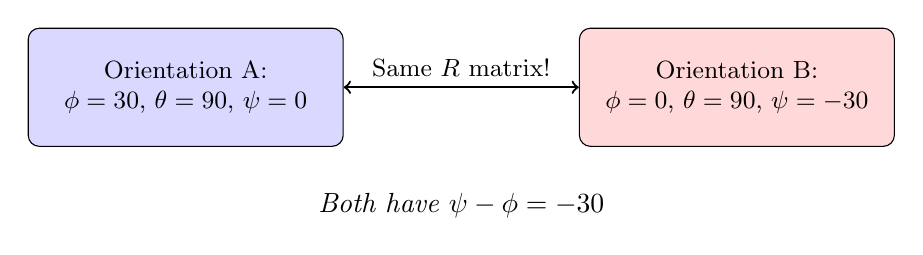
\begin{tikzpicture}[every node/.style={font=\small}]
    % Two orientations
    \node[draw, rectangle, rounded corners, fill=blue!15, minimum width=4cm, minimum height=1.5cm, align=center] (A) at (0, 0) {Orientation A:\\$\phi = 30°$, $\theta = 90°$, $\psi = 0°$};
    \node[draw, rectangle, rounded corners, fill=red!15, minimum width=4cm, minimum height=1.5cm, align=center] (B) at (7, 0) {Orientation B:\\$\phi = 0°$, $\theta = 90°$, $\psi = -30°$};

    % Arrow showing equivalence
    \draw[thick, <->] (A) -- node[above] {Same $R$ matrix!} (B);

    % Note below
    \node[below of=A, yshift=-0.5cm, xshift=3.5cm, font=\itshape] {Both have $\psi - \phi = -30°$};
\end{tikzpicture}
\end{center}

\textbf{Numerical demonstration}: Both orientations produce the \emph{identical} rotation matrix:
\begin{equation}
R = \begin{bmatrix} 0 & -0.5 & 0.866 \\ 0 & 0.866 & 0.5 \\ -1 & 0 & 0 \end{bmatrix}
\end{equation}

If we try to extract Euler angles from this matrix using the standard formulas:
\begin{align}
\theta &= -\arcsin(R_{31}) = -\arcsin(-1) = 90° \quad \checkmark \\
\phi &= \text{atan2}(R_{32}, R_{33}) = \text{atan2}(0, 0) \quad \text{\textbf{undefined!}} \\
\psi &= \text{atan2}(R_{21}, R_{11}) = \text{atan2}(0, 0) \quad \text{\textbf{undefined!}}
\end{align}

\begin{warningbox}
At $\theta = \pm 90°$, one degree of freedom is lost. We cannot distinguish between ``rolled then pitched up'' and ``pitched up then yawed.'' The atan2$(0, 0)$ calculation is undefined, and any numerical implementation will produce arbitrary or unstable results.
\end{warningbox}

\paragraph{The Quaternion Solution}

The same maneuver using quaternions has no such problem. Starting from the identity orientation:
\begin{enumerate}
    \item Initial orientation: $\mathbf{q}_0 = [1, 0, 0, 0]^T$
    \item Pitch up 90°: $\mathbf{q}_{\text{pitch}} = [\cos(45°), 0, \sin(45°), 0]^T = [0.707, 0, 0.707, 0]^T$
    \item After pitch: $\mathbf{q}_1 = \mathbf{q}_{\text{pitch}} \otimes \mathbf{q}_0 = [0.707, 0, 0.707, 0]^T$
    \item Roll 30° about body x-axis: $\mathbf{q}_{\text{roll}} = [0.966, 0.259, 0, 0]^T$
    \item Final: $\mathbf{q}_2 = \mathbf{q}_1 \otimes \mathbf{q}_{\text{roll}} = [0.683, 0.183, 0.683, 0.183]^T$
\end{enumerate}

The quaternion $\mathbf{q}_2 = [0.683, 0.183, 0.683, 0.183]^T$ is:
\begin{itemize}
    \item \textbf{Unique}: No other unit quaternion represents this orientation (except $-\mathbf{q}_2$, which represents the same rotation)
    \item \textbf{Well-defined}: No division by zero, no undefined operations
    \item \textbf{Composable}: We can continue applying rotations without any singularity
\end{itemize}

Converting this quaternion to a rotation matrix gives a valid, well-defined result:
\begin{equation}
R = \begin{bmatrix} 0.067 & -0.5 & 0.863 \\ 0.25 & 0.866 & 0.433 \\ -0.966 & 0.0 & 0.259 \end{bmatrix}
\end{equation}

This matrix can be used to transform vectors correctly, even though we passed through $\theta = 90°$.

%----------------------------------------------------------------------
\subsubsection{Part 3: Practical Implications for Quadrotor Control}

\paragraph{When Gimbal Lock Matters}

\begin{itemize}
    \item \textbf{Aerobatic maneuvers}: Flips, loops, and rolls pass through $\theta = \pm 90°$
    \item \textbf{Aggressive recovery}: A tumbling quadrotor may have any orientation
    \item \textbf{Continuous tracking}: Numerical integration of angular velocity can drift through singularities
\end{itemize}

\paragraph{When Euler Angles Are Fine}

\begin{itemize}
    \item \textbf{Normal flight}: Hover and forward flight typically have $|\theta| < 30°$
    \item \textbf{Display and logging}: Humans understand ``roll = 10°, pitch = 5°'' more easily than quaternion components
    \item \textbf{Small-angle control}: Near hover, Euler angle controllers work well
\end{itemize}

\begin{keyidea}[title=Best Practice for Quadrotor Software]
\begin{enumerate}
    \item \textbf{Store orientation internally as a quaternion}---no singularities, efficient composition
    \item \textbf{Perform sensor fusion using quaternions}---avoid gimbal lock in Kalman filters
    \item \textbf{Convert to Euler angles only for display}---let pilots see familiar roll/pitch/yaw values
    \item \textbf{Use rotation matrices for vector transformations}---efficient for sensor frame conversions
\end{enumerate}
\end{keyidea}

\begin{center}
\begin{tikzpicture}[every node/.style={font=\small},
    block/.style={draw, rectangle, rounded corners, minimum width=3cm, minimum height=1cm, align=center}]

    \node[block, fill=green!20] (sensors) at (0, 0) {IMU Data\\(angular rates)};
    \node[block, fill=blue!20] (quat) at (5, 0) {Quaternion\\(internal state)};
    \node[block, fill=yellow!20] (euler) at (10, 0) {Euler Angles\\(display only)};

    \draw[-{Stealth}, thick] (sensors) -- node[above] {integrate} (quat);
    \draw[-{Stealth}, thick] (quat) -- node[above] {convert} (euler);

    \node[below of=quat, yshift=0.3cm, font=\footnotesize\itshape] {No singularities here};
    \node[below of=euler, yshift=0.3cm, font=\footnotesize\itshape] {Human-readable};
\end{tikzpicture}
\end{center}

%======================================================================

\section{Homogeneous Transformations}
\label{sec:homogeneous-transformations}

\subsection{Motivation: Combining Rotation and Translation}

So far, we have treated rotation and translation separately. To transform a point $\mathbf{p}^B$ from the body frame to the world frame, we must:
\begin{enumerate}
    \item Rotate the point: $R^W_B \, \mathbf{p}^B$
    \item Add the translation: $R^W_B \, \mathbf{p}^B + \mathbf{t}^W_B$
\end{enumerate}

This two-step process becomes cumbersome when chaining multiple transformations. For example, transforming through three frames requires:
\[
\mathbf{p}^A = R^A_B \left( R^B_C \, \mathbf{p}^C + \mathbf{t}^B_C \right) + \mathbf{t}^A_B
\]

\textbf{Homogeneous transformations} provide an elegant solution: by embedding the 3D transformation in a $4 \times 4$ matrix, both rotation and translation can be performed with a single matrix multiplication.

\subsection{The Homogeneous Transformation Matrix}

\begin{definition}[Homogeneous Transformation Matrix]
\index{homogeneous transformation}
The homogeneous transformation matrix $T^j_i \in \mathbb{R}^{4 \times 4}$ combines the rotation $R^j_i$ and translation $\mathbf{t}^j_i$ into a single matrix:
\begin{equation}
T^j_i = \begin{bmatrix} R^j_i & \mathbf{t}^j_i \\ \mathbf{0}^T & 1 \end{bmatrix}
= \begin{bmatrix}
r_{11} & r_{12} & r_{13} & t_x \\
r_{21} & r_{22} & r_{23} & t_y \\
r_{31} & r_{32} & r_{33} & t_z \\
0 & 0 & 0 & 1
\end{bmatrix}
\end{equation}
where:
\begin{itemize}
    \item $R^j_i \in \mathbb{R}^{3 \times 3}$: rotation matrix (upper-left $3 \times 3$ block)
    \item $\mathbf{t}^j_i \in \mathbb{R}^{3}$: translation vector (upper-right column)
    \item $\mathbf{0}^T = [0, 0, 0]$: bottom row padding
    \item The subscript $i$ is the source frame, superscript $j$ is the reference frame
\end{itemize}
\end{definition}

For the quadrotor, the transformation from body frame $\{B\}$ to world frame $\{W\}$ is:
\begin{equation}
T^W_B = \begin{bmatrix} R^W_B & \mathbf{t}^W_B \\ \mathbf{0}^T & 1 \end{bmatrix}
\end{equation}
where $\mathbf{t}^W_B = [x, y, z]^T$ is the position of the quadrotor (body frame origin) in world coordinates.

\subsection{Homogeneous Coordinates}

To use the $4 \times 4$ matrix, we extend 3D points to \textbf{homogeneous coordinates} by appending a 1:
\[
\mathbf{p} = \begin{bmatrix} p_x \\ p_y \\ p_z \end{bmatrix}
\quad \rightarrow \quad
\tilde{\mathbf{p}} = \begin{bmatrix} p_x \\ p_y \\ p_z \\ 1 \end{bmatrix}
\]

The transformation then becomes a single matrix multiplication:
\begin{equation}
\begin{bmatrix} \mathbf{p}^W \\ 1 \end{bmatrix} = T^W_B \begin{bmatrix} \mathbf{p}^B \\ 1 \end{bmatrix}
\end{equation}

\begin{example}[Transforming a Point on the Quadrotor]
Consider a sensor mounted on the quadrotor at position $\mathbf{p}^B = [0.1, 0, -0.05]^T$ in body coordinates (10 cm forward, 5 cm up from the center of mass). The quadrotor is at position $\mathbf{t}^W_B = [2, 3, -10]^T$ in world coordinates (2m North, 3m East, 10m altitude in NED) with orientation $\phi = 0°$, $\theta = 15°$, $\psi = 45°$.

\textbf{Step 1}: Compute the rotation matrix $R^W_B$ for the given Euler angles.

With $c_\alpha = \cos\alpha$, $s_\alpha = \sin\alpha$, and using $\cos 15° = \frac{\sqrt{6}+\sqrt{2}}{4}$, $\sin 15° = \frac{\sqrt{6}-\sqrt{2}}{4}$, $\cos 45° = \sin 45° = \frac{\sqrt{2}}{2}$:

For simplicity, we use decimal approximations: $c_{15} \approx 0.966$, $s_{15} \approx 0.259$, $c_{45} = s_{45} \approx 0.707$.

Since $\phi = 0$: $c_\phi = 1$, $s_\phi = 0$.

\[
R^W_B = \begin{bmatrix}
c_\psi c_\theta & -s_\psi & c_\psi s_\theta \\
s_\psi c_\theta & c_\psi & s_\psi s_\theta \\
-s_\theta & 0 & c_\theta
\end{bmatrix}
= \begin{bmatrix}
0.683 & -0.707 & 0.183 \\
0.683 & 0.707 & 0.183 \\
-0.259 & 0 & 0.966
\end{bmatrix}
\]

\textbf{Step 2}: Construct the homogeneous transformation matrix:
\[
T^W_B = \begin{bmatrix}
0.683 & -0.707 & 0.183 & 2 \\
0.683 & 0.707 & 0.183 & 3 \\
-0.259 & 0 & 0.966 & -10 \\
0 & 0 & 0 & 1
\end{bmatrix}
\]

\textbf{Step 3}: Transform the sensor position:
\[
\begin{bmatrix} \mathbf{p}^W \\ 1 \end{bmatrix}
= T^W_B \begin{bmatrix} 0.1 \\ 0 \\ -0.05 \\ 1 \end{bmatrix}
= \begin{bmatrix}
0.683 \cdot 0.1 + (-0.707) \cdot 0 + 0.183 \cdot (-0.05) + 2 \\
0.683 \cdot 0.1 + 0.707 \cdot 0 + 0.183 \cdot (-0.05) + 3 \\
-0.259 \cdot 0.1 + 0 \cdot 0 + 0.966 \cdot (-0.05) + (-10) \\
1
\end{bmatrix}
\]
\[
= \begin{bmatrix}
0.0683 - 0.0092 + 2 \\
0.0683 - 0.0092 + 3 \\
-0.0259 - 0.0483 - 10 \\
1
\end{bmatrix}
= \begin{bmatrix}
2.059 \\
3.059 \\
-10.074 \\
1
\end{bmatrix}
\]

The sensor is at world position $\mathbf{p}^W \approx [2.06, 3.06, -10.07]^T$ meters---slightly ahead of and above the quadrotor center.
\end{example}

\subsection{Composing Transformations}

A key advantage of homogeneous transformations is that \textbf{chaining transformations} reduces to matrix multiplication:

\begin{equation}
T^A_C = T^A_B \cdot T^B_C
\end{equation}

This follows from the associativity of matrix multiplication. Transforming a point through multiple frames:
\[
\tilde{\mathbf{p}}^A = T^A_B \, \tilde{\mathbf{p}}^B = T^A_B \left( T^B_C \, \tilde{\mathbf{p}}^C \right) = \left( T^A_B \cdot T^B_C \right) \tilde{\mathbf{p}}^C = T^A_C \, \tilde{\mathbf{p}}^C
\]

\begin{example}[Chaining Transformations: Camera on a Gimbal]
Consider a camera mounted on a 2-axis gimbal attached to the quadrotor. We have three frames:
\begin{itemize}
    \item $\{W\}$: World frame (NED)
    \item $\{B\}$: Body frame (quadrotor center of mass)
    \item $\{C\}$: Camera frame (at the gimbal)
\end{itemize}

The gimbal is mounted 15 cm below the quadrotor center: $\mathbf{t}^B_C = [0, 0, 0.15]^T$ (in body coordinates, positive $z$ is down).

The gimbal tilts the camera $20°$ nose-down (pitch only, no roll or yaw relative to body):
\[
R^B_C = R_y(20°) = \begin{bmatrix}
\cos 20° & 0 & \sin 20° \\
0 & 1 & 0 \\
-\sin 20° & 0 & \cos 20°
\end{bmatrix}
\approx \begin{bmatrix}
0.940 & 0 & 0.342 \\
0 & 1 & 0 \\
-0.342 & 0 & 0.940
\end{bmatrix}
\]

Thus:
\[
T^B_C = \begin{bmatrix}
0.940 & 0 & 0.342 & 0 \\
0 & 1 & 0 & 0 \\
-0.342 & 0 & 0.940 & 0.15 \\
0 & 0 & 0 & 1
\end{bmatrix}
\]

If the quadrotor is hovering level at $\mathbf{t}^W_B = [0, 0, -5]^T$ (5m altitude) with $\psi = 90°$ (facing East):
\[
T^W_B = \begin{bmatrix}
0 & -1 & 0 & 0 \\
1 & 0 & 0 & 0 \\
0 & 0 & 1 & -5 \\
0 & 0 & 0 & 1
\end{bmatrix}
\]

The camera-to-world transformation is:
\[
T^W_C = T^W_B \cdot T^B_C =
\begin{bmatrix}
0 & -1 & 0 & 0 \\
1 & 0 & 0 & 0 \\
0 & 0 & 1 & -5 \\
0 & 0 & 0 & 1
\end{bmatrix}
\begin{bmatrix}
0.940 & 0 & 0.342 & 0 \\
0 & 1 & 0 & 0 \\
-0.342 & 0 & 0.940 & 0.15 \\
0 & 0 & 0 & 1
\end{bmatrix}
\]
\[
= \begin{bmatrix}
0 & -1 & 0 & 0 \\
0.940 & 0 & 0.342 & 0 \\
-0.342 & 0 & 0.940 & -4.85 \\
0 & 0 & 0 & 1
\end{bmatrix}
\]

A point directly in front of the camera at distance 1m ($\mathbf{p}^C = [0, 0, 1]^T$ in camera coordinates) is at world position:
\[
\tilde{\mathbf{p}}^W = T^W_C \begin{bmatrix} 0 \\ 0 \\ 1 \\ 1 \end{bmatrix}
= \begin{bmatrix} 0 \\ 0.342 \\ -4.85 + 0.940 \\ 1 \end{bmatrix}
= \begin{bmatrix} 0 \\ 0.342 \\ -3.91 \\ 1 \end{bmatrix}
\]

The point is at $[0, 0.34, -3.91]^T$: slightly East and at 3.91m altitude (the camera is looking down and forward).
\end{example}

\subsection{Inverse of a Homogeneous Transformation}

The inverse transformation $T^B_W = (T^W_B)^{-1}$ transforms points from world frame to body frame. Rather than computing a general $4 \times 4$ matrix inverse, we can use the structure:

\begin{equation}
T^B_W = (T^W_B)^{-1} = \begin{bmatrix} (R^W_B)^T & -(R^W_B)^T \mathbf{t}^W_B \\ \mathbf{0}^T & 1 \end{bmatrix}
= \begin{bmatrix} R^B_W & -R^B_W \mathbf{t}^W_B \\ \mathbf{0}^T & 1 \end{bmatrix}
\end{equation}

\begin{keyidea}[title=Why This Formula Works]
To invert the transformation ``rotate then translate,'' we must ``translate back then rotate back'':
\begin{enumerate}
    \item The inverse rotation is $R^B_W = (R^W_B)^T$
    \item The translation $\mathbf{t}^W_B$ was applied \emph{after} rotation, so to undo it we must first subtract it, then rotate back: $-R^B_W \mathbf{t}^W_B$
\end{enumerate}
\end{keyidea}

\begin{example}[Computing the Inverse Transformation]
Given the quadrotor at position $\mathbf{t}^W_B = [2, 3, -10]^T$ with a simple $90°$ yaw rotation:
\[
R^W_B = R_z(90°) = \begin{bmatrix} 0 & -1 & 0 \\ 1 & 0 & 0 \\ 0 & 0 & 1 \end{bmatrix}, \quad
T^W_B = \begin{bmatrix} 0 & -1 & 0 & 2 \\ 1 & 0 & 0 & 3 \\ 0 & 0 & 1 & -10 \\ 0 & 0 & 0 & 1 \end{bmatrix}
\]

The inverse is:
\[
R^B_W = (R^W_B)^T = \begin{bmatrix} 0 & 1 & 0 \\ -1 & 0 & 0 \\ 0 & 0 & 1 \end{bmatrix}
\]
\[
-R^B_W \mathbf{t}^W_B = -\begin{bmatrix} 0 & 1 & 0 \\ -1 & 0 & 0 \\ 0 & 0 & 1 \end{bmatrix} \begin{bmatrix} 2 \\ 3 \\ -10 \end{bmatrix}
= -\begin{bmatrix} 3 \\ -2 \\ -10 \end{bmatrix}
= \begin{bmatrix} -3 \\ 2 \\ 10 \end{bmatrix}
\]
\[
T^B_W = \begin{bmatrix} 0 & 1 & 0 & -3 \\ -1 & 0 & 0 & 2 \\ 0 & 0 & 1 & 10 \\ 0 & 0 & 0 & 1 \end{bmatrix}
\]

\textbf{Verification}: A point at the world origin $\mathbf{p}^W = [0, 0, 0]^T$ should transform to the quadrotor's view of the origin:
\[
\tilde{\mathbf{p}}^B = T^B_W \begin{bmatrix} 0 \\ 0 \\ 0 \\ 1 \end{bmatrix} = \begin{bmatrix} -3 \\ 2 \\ 10 \\ 1 \end{bmatrix}
\]
From the quadrotor's perspective (facing East after $90°$ yaw), the world origin is 3m to the left, 2m forward, and 10m below---which matches our setup.
\end{example}

\begin{notebox}[title=When to Use Homogeneous Transformations]
Homogeneous transformations are essential when:
\begin{itemize}
    \item Chaining multiple coordinate frame transformations
    \item Working with robotic manipulators (each joint adds a transformation)
    \item Computer graphics and visualization
    \item Sensor fusion involving multiple sensor mounting positions
\end{itemize}
For pure rotation problems (like attitude estimation), the $3 \times 3$ rotation matrix or quaternion representation is more efficient.
\end{notebox}

\chapter{Inertial Sensors and Measurement Models}

%----------------------------------------------------------------------
% FIGURE: IMU Sensor Package Overview
%----------------------------------------------------------------------
\begin{figure}[htbp]
\centering
\begin{tikzpicture}[scale=0.9]
    % Main IMU chip (3D box)
    \begin{scope}[shift={(-3,0)}]
        % Chip body
        \fill[gray!20] (0,0) rectangle (4,3);
        \draw[thick] (0,0) rectangle (4,3);

        % 3D effect
        \fill[gray!30] (4,0) -- (4.5,0.5) -- (4.5,3.5) -- (4,3) -- cycle;
        \fill[gray!10] (0,3) -- (0.5,3.5) -- (4.5,3.5) -- (4,3) -- cycle;
        \draw[thick] (4,0) -- (4.5,0.5) -- (4.5,3.5) -- (4,3);
        \draw[thick] (0,3) -- (0.5,3.5) -- (4.5,3.5);

        % Internal blocks
        % Accelerometer
        \fill[xaxis!20] (0.3,1.8) rectangle (1.8,2.7);
        \draw[xaxis] (0.3,1.8) rectangle (1.8,2.7);
        \node[font=\tiny, text width=1.3cm, align=center] at (1.05,2.25) {3-axis\\Accel};

        % Gyroscope
        \fill[yaxis!20] (2.2,1.8) rectangle (3.7,2.7);
        \draw[yaxis] (2.2,1.8) rectangle (3.7,2.7);
        \node[font=\tiny, text width=1.3cm, align=center] at (2.95,2.25) {3-axis\\Gyro};

        % Magnetometer (optional)
        \fill[zaxis!20] (1.25,0.3) rectangle (2.75,1.2);
        \draw[zaxis] (1.25,0.3) rectangle (2.75,1.2);
        \node[font=\tiny, text width=1.3cm, align=center] at (2,0.75) {3-axis\\Mag};

        % Body frame axes
        \draw[xaxisstyle, thin] (0.2,0.2) -- (1,0.2) node[right, font=\tiny] {$x_B$};
        \draw[yaxisstyle, thin] (0.2,0.2) -- (0.2,1) node[above, font=\tiny] {$y_B$};

        % Chip label
        \node[font=\scriptsize\bfseries] at (2,3.8) {9-DOF IMU};

        % Output signals
        \draw[->, thick] (4.5,2.5) -- (5.5,2.5) node[right, font=\tiny] {$\omega_x, \omega_y, \omega_z$};
        \draw[->, thick] (4.5,1.5) -- (5.5,1.5) node[right, font=\tiny] {$a_x, a_y, a_z$};
        \draw[->, thick] (4.5,0.5) -- (5.5,0.5) node[right, font=\tiny] {$m_x, m_y, m_z$};
    \end{scope}

    % MEMS principle inset
    \begin{scope}[shift={(5,-0.5)}]
        \draw[thick, rounded corners] (-0.3,-0.3) rectangle (3.3,3.3);
        \node[font=\scriptsize\bfseries] at (1.5,3) {MEMS Principle};

        % Housing
        \draw[thick, fill=gray!20] (0,0.5) -- (0,2) -- (0.3,2) -- (0.3,0.5) -- cycle;
        \draw[thick, fill=gray!20] (2.7,0.5) -- (2.7,2) -- (3,2) -- (3,0.5) -- cycle;

        % Springs
        \draw[thick, decorate, decoration={zigzag, segment length=3mm, amplitude=1mm}]
            (0.3,1.25) -- (1,1.25);
        \draw[thick, decorate, decoration={zigzag, segment length=3mm, amplitude=1mm}]
            (2,1.25) -- (2.7,1.25);

        % Proof mass
        \fill[orange!40] (1,0.8) rectangle (2,1.7);
        \draw[thick] (1,0.8) rectangle (2,1.7);
        \node[font=\tiny] at (1.5,1.25) {mass};

        % Capacitor plates
        \draw[thick, blue!60] (0.5,0.5) -- (0.5,2);
        \draw[thick, blue!60] (2.5,0.5) -- (2.5,2);
        \node[font=\tiny, blue!60] at (0.5,0.2) {C1};
        \node[font=\tiny, blue!60] at (2.5,0.2) {C2};

        % Acceleration arrow
        \draw[-{Stealth}, very thick, red!70] (3.5,1.25) -- (4.2,1.25)
            node[right, font=\tiny] {$a$};

        % Annotation
        \node[font=\tiny, text width=2.5cm, align=center] at (1.5,-0.6) {Mass displacement\\$\rightarrow$ capacitance change};
    \end{scope}

    % Size comparison
    \node[font=\scriptsize, text width=4cm, align=center] at (1,-1.5) {
        Typical size: $3\times3\times1$ mm\\
        (smaller than a fingernail!)
    };
\end{tikzpicture}
\caption{Inertial Measurement Unit (IMU) overview. Left: A 9-DOF IMU contains a 3-axis accelerometer, gyroscope, and magnetometer. Right: MEMS accelerometers measure displacement of a proof mass suspended by springs.}
\label{fig:imu-overview}
\end{figure}
%----------------------------------------------------------------------

\section{Introduction: How Do We Measure Orientation?}

In the previous chapter, we developed the mathematics for describing orientation. Now we ask: how do we \emph{measure} orientation in practice?

The answer involves \textbf{inertial sensors}---devices that measure motion without external references (like GPS satellites or visual landmarks). These are crucial because they work everywhere: indoors, underground, in space, or when GPS is jammed.

\begin{keyidea}[title=The Fundamental Challenge]
No single sensor directly measures orientation. Instead, we measure \emph{related quantities} (angular velocity, acceleration, magnetic field) and must \emph{compute} orientation from these. Each sensor has strengths and weaknesses; combining them intelligently is the art of sensor fusion.
\end{keyidea}

For a comprehensive tutorial on using inertial sensors for position and orientation estimation, see Kok et al.~\cite{kok2017using}.

\section{The Inertial Measurement Unit (IMU)}
\index{IMU (Inertial Measurement Unit)}

An IMU\index{IMU (Inertial Measurement Unit)|textbf} is a sensor package typically containing:
\begin{itemize}
    \item \textbf{3-axis accelerometer}\index{accelerometer}: Measures specific force (acceleration + gravity)
    \item \textbf{3-axis gyroscope}\index{gyroscope}: Measures angular velocity
    \item \textbf{3-axis magnetometer}\index{magnetometer} (in 9-DOF IMUs): Measures magnetic field
\end{itemize}

Modern MEMS (Micro-Electro-Mechanical Systems) IMUs are remarkably small and cheap---your smartphone contains one. The Crazyflie uses the BMI088 (accel+gyro) and similar sensors.

\begin{notebox}[title=Assumption: Sensor Location]
We assume the IMU is located at the quadrotor's center of gravity. If not, centripetal accelerations during rotation would affect the accelerometer readings. For small quadrotors like the Crazyflie, this error is typically negligible.
\end{notebox}

\section{Gyroscope}

\subsection{What Does a Gyroscope Measure?}

\begin{definition}[Gyroscope Measurement]
An ideal gyroscope measures the \textbf{angular velocity} of the body frame relative to an inertial frame, expressed in body coordinates:
\[
\boldsymbol{\omega} = \begin{bmatrix} p \\ q \\ r \end{bmatrix}
\]
where $p$, $q$, $r$ are rotation rates about the body $x$, $y$, $z$ axes (roll rate, pitch rate, yaw rate).
\end{definition}

\textbf{Intuition}: The gyroscope tells you ``how fast am I rotating right now?''---not ``what is my orientation?''

\subsection{Realistic Measurement Model}

Real gyroscopes don't measure perfect angular velocity. The measurement is corrupted:

\begin{equation}
\boldsymbol{\omega}_{meas} = \boldsymbol{\omega}_{true} + \mathbf{b}_g(t) + \mathbf{n}_g
\end{equation}

\begin{notebox}[title=Gyroscope Error Sources]
\begin{itemize}
    \item $\mathbf{b}_g(t)$: \textbf{Bias}---a slowly-varying offset. Even when stationary, the gyro reports a small non-zero reading. Bias can drift due to temperature changes or aging.
    \item $\mathbf{n}_g$: \textbf{White noise}---rapid random fluctuations, typically modeled as zero-mean Gaussian
\end{itemize}
\end{notebox}

\begin{definition}[Gyroscope Noise Parameters]
\begin{itemize}
    \item \textbf{Angular Random Walk (ARW)}: Noise density, in units of $°/\sqrt{h}$ or $°/s/\sqrt{Hz}$
    \item \textbf{Bias Instability}: How much the bias drifts, in $°/h$
\end{itemize}
\end{definition}

\subsection{The Drift Problem}

To get orientation from angular velocity, we integrate:
\begin{equation}
\theta(t) = \theta_0 + \int_0^t \omega(\tau) \, d\tau
\end{equation}

\begin{warningbox}[title=Integration Amplifies Errors]
Integration is mathematically beautiful but practically treacherous:
\begin{itemize}
    \item \textbf{Bias}: A constant bias $b$ causes error that grows \textbf{linearly}: $\epsilon(t) = b \cdot t$
    \item \textbf{White noise}: Random noise causes a \textbf{random walk}: $\epsilon(t) \propto \sqrt{t}$
\end{itemize}
After enough time, the estimated orientation diverges arbitrarily far from truth.
\end{warningbox}

%----------------------------------------------------------------------
% FIGURE: Gyroscope Drift Over Time
%----------------------------------------------------------------------
\begin{figure}[htbp]
\centering
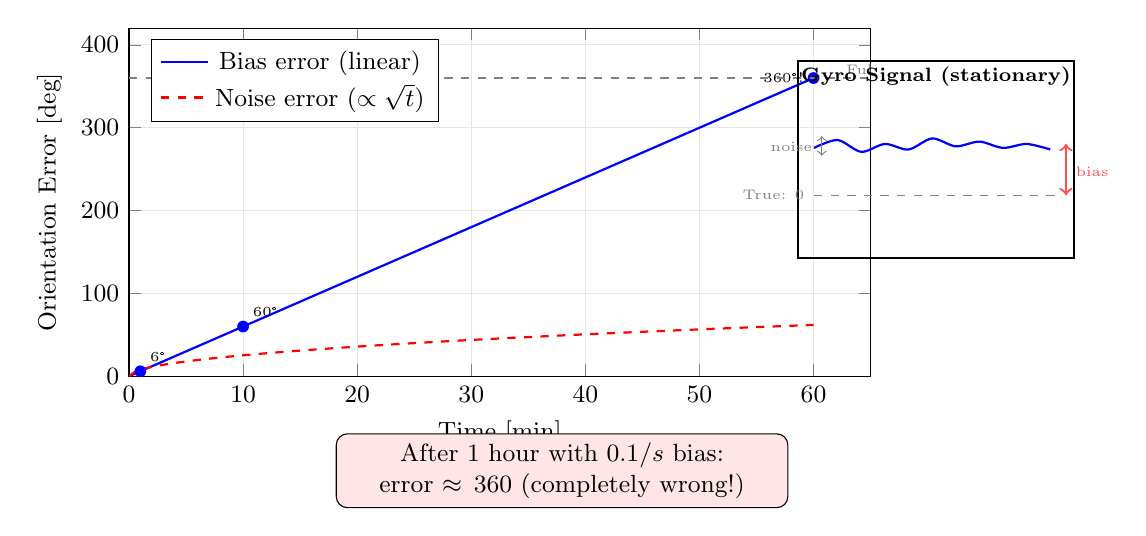
\begin{tikzpicture}
    \begin{axis}[
        width=11cm,
        height=6cm,
        xlabel={Time [min]},
        ylabel={Orientation Error [deg]},
        xmin=0, xmax=65,
        ymin=0, ymax=420,
        grid=both,
        grid style={gray!20},
        legend pos=north west,
        legend style={font=\small},
        every axis label/.style={font=\small},
        tick label style={font=\small}
    ]
        % Bias error (linear): 0.1 deg/s = 6 deg/min
        \addplot[thick, blue, domain=0:60, samples=100] {6*x};
        \addlegendentry{Bias error (linear)}

        % Noise error (random walk): sqrt growth, scaled
        \addplot[thick, red, dashed, domain=0:60, samples=100] {8*sqrt(x)};
        \addlegendentry{Noise error ($\propto\sqrt{t}$)}

        % Mark key points
        \node[circle, fill=blue, inner sep=1.5pt] at (axis cs:1,6) {};
        \node[above right, font=\tiny] at (axis cs:1,6) {6°};

        \node[circle, fill=blue, inner sep=1.5pt] at (axis cs:10,60) {};
        \node[above right, font=\tiny] at (axis cs:10,60) {60°};

        \node[circle, fill=blue, inner sep=1.5pt] at (axis cs:60,360) {};
        \node[left, font=\tiny] at (axis cs:60,360) {360°!};

        % Horizontal reference line at 360 deg
        \draw[gray, dashed] (axis cs:0,360) -- (axis cs:65,360);
        \node[right, font=\tiny, gray] at (axis cs:62,370) {Full rotation};

    \end{axis}

    % Inset: Gyro signal
    \begin{scope}[shift={(8.5,1.5)}]
        \draw[thick] (0,0) rectangle (3.5,2.5);
        \node[font=\scriptsize\bfseries] at (1.75,2.3) {Gyro Signal (stationary)};

        % True value (zero)
        \draw[dashed, gray] (0.2,0.8) -- (3.3,0.8);
        \node[font=\tiny, gray, left] at (0.2,0.8) {True: 0};

        % Measured signal with bias and noise
        \draw[thick, blue] plot[smooth, tension=0.5] coordinates {
            (0.2,1.4) (0.5,1.5) (0.8,1.35) (1.1,1.45) (1.4,1.38)
            (1.7,1.52) (2.0,1.42) (2.3,1.48) (2.6,1.4) (2.9,1.45) (3.2,1.38)
        };

        % Bias indicator
        \draw[<->, thick, red!70] (3.4,0.8) -- (3.4,1.45);
        \node[font=\tiny, red!70, right] at (3.4,1.1) {bias};

        % Noise band
        \draw[<->, gray] (0.3,1.3) -- (0.3,1.55);
        \node[font=\tiny, gray, left] at (0.3,1.42) {noise};
    \end{scope}

    % Annotation
    \node[draw, rounded corners, fill=red!10, font=\small, text width=5.5cm, align=center]
        at (5.5,-1.2) {
        After 1 hour with $0.1°/s$ bias:\\
        error $\approx 360°$ (completely wrong!)
    };
\end{tikzpicture}
\caption{Gyroscope drift over time. A bias of $0.1°/s$ (typical for consumer MEMS) causes orientation error to grow linearly, reaching $360°$ after one hour. Noise causes additional random walk error that grows as $\sqrt{t}$.}
\label{fig:gyro-drift}
\end{figure}
%----------------------------------------------------------------------

\begin{example}[Drift Calculation]
Consider a MEMS gyroscope with bias $b = 0.1°/s$ (typical for consumer-grade sensors).

After 1 minute: orientation error $\approx 0.1 \times 60 = 6°$

After 10 minutes: orientation error $\approx 60°$

After 1 hour: orientation error $\approx 360°$ (completely wrong!)
\end{example}

\begin{keyidea}[title=Gyroscope Summary]
The gyroscope is \textbf{excellent for short-term, high-frequency orientation changes} but \textbf{useless for long-term absolute orientation} due to drift. We need another sensor to provide an absolute reference.
\end{keyidea}

\section{Accelerometer}

\subsection{What Does an Accelerometer Measure?}

This is surprisingly subtle. An accelerometer does \emph{not} directly measure acceleration!

\begin{definition}[Specific Force]
An accelerometer measures \textbf{specific force}---the non-gravitational force per unit mass, or equivalently, the acceleration you would ``feel'' if you were a test mass inside the sensor.
\end{definition}

In the body frame:
\begin{equation}
\mathbf{f}_{meas} = R^B_W (\mathbf{a}_{body} - \mathbf{g}) + \mathbf{b}_a + \mathbf{n}_a
\end{equation}

where:
\begin{itemize}
    \item $\mathbf{a}_{body}$: True acceleration of the body in the world frame
    \item $\mathbf{g} = [0, 0, g]^T$: Gravity vector in world frame (NED: points down)
    \item $R^B_W$: Rotation from world to body frame
    \item $\mathbf{b}_a$, $\mathbf{n}_a$: Bias and noise (similar to gyroscope)
\end{itemize}

%----------------------------------------------------------------------
% FIGURE: Accelerometer Specific Force (Spring-Mass Analogy)
%----------------------------------------------------------------------
\begin{figure}[htbp]
\centering
\begin{tikzpicture}[scale=0.85]
    % === Panel 1: Stationary on ground ===
    \begin{scope}[shift={(-5,0)}]
        \node[font=\bfseries\small] at (0,3.5) {At Rest};

        % Ground
        \fill[brown!20] (-1.5,-1.5) rectangle (1.5,-1.2);
        \draw[thick] (-1.5,-1.2) -- (1.5,-1.2);

        % Accelerometer case
        \draw[very thick, fill=gray!10] (-1,-1.2) rectangle (1,1.8);

        % Spring (stretched)
        \draw[thick, decorate, decoration={zigzag, segment length=2.5mm, amplitude=1.5mm}]
            (0,1.5) -- (0,0.3);

        % Proof mass (displaced down)
        \fill[orange!60] (-0.4,-0.3) rectangle (0.4,0.3);
        \draw[thick] (-0.4,-0.3) rectangle (0.4,0.3);
        \node[font=\tiny] at (0,0) {m};

        % Gravity arrow on mass
        \draw[-{Stealth}, very thick, blue!70] (0.6,0) -- (0.6,-0.8)
            node[right, font=\scriptsize] {$mg$};

        % Output reading
        \node[draw, rounded corners, fill=green!20, font=\scriptsize] at (0,-2.2)
            {Output: $f = +g$};

        % Annotation
        \node[font=\tiny, text width=2.2cm, align=center] at (0,-3) {No motion, but\\reads $g$!};
    \end{scope}

    % === Panel 2: Free fall ===
    \begin{scope}[shift={(0,0)}]
        \node[font=\bfseries\small] at (0,3.5) {Free Fall};

        % Motion blur / falling indicator
        \draw[-{Stealth}, very thick, red!70] (1.3,1.5) -- (1.3,-0.5)
            node[right, font=\scriptsize] {falling};

        % Accelerometer case
        \draw[very thick, fill=gray!10] (-1,-1.2) rectangle (1,1.8);

        % Spring (relaxed - not stretched)
        \draw[thick, decorate, decoration={zigzag, segment length=4mm, amplitude=1mm}]
            (0,1.5) -- (0,0.8);

        % Proof mass (centered - no displacement!)
        \fill[orange!60] (-0.4,0.2) rectangle (0.4,0.8);
        \draw[thick] (-0.4,0.2) rectangle (0.4,0.8);
        \node[font=\tiny] at (0,0.5) {m};

        % Both falling together
        \node[font=\tiny, gray] at (0,-0.5) {(both fall at $g$)};

        % Output reading
        \node[draw, rounded corners, fill=yellow!30, font=\scriptsize] at (0,-2.2)
            {Output: $f = 0$};

        % Annotation
        \node[font=\tiny, text width=2.2cm, align=center] at (0,-3) {Accelerating at $g$,\\but reads 0!};
    \end{scope}

    % === Panel 3: Accelerating upward ===
    \begin{scope}[shift={(5,0)}]
        \node[font=\bfseries\small] at (0,3.5) {Accelerating Up};

        % Motion indicator
        \draw[-{Stealth}, very thick, green!60!black] (1.3,-0.5) -- (1.3,1.5)
            node[right, font=\scriptsize] {$a$};

        % Accelerometer case
        \draw[very thick, fill=gray!10] (-1,-1.2) rectangle (1,1.8);

        % Spring (more stretched)
        \draw[thick, decorate, decoration={zigzag, segment length=2mm, amplitude=2mm}]
            (0,1.5) -- (0,-0.1);

        % Proof mass (displaced further down)
        \fill[orange!60] (-0.4,-0.7) rectangle (0.4,-0.1);
        \draw[thick] (-0.4,-0.7) rectangle (0.4,-0.1);
        \node[font=\tiny] at (0,-0.4) {m};

        % Output reading
        \node[draw, rounded corners, fill=blue!20, font=\scriptsize] at (0,-2.2)
            {Output: $f = a + g$};

        % Annotation
        \node[font=\tiny, text width=2.2cm, align=center] at (0,-3) {More than $1g$\\reading};
    \end{scope}

    % Key insight box at bottom
    \node[draw, rounded corners, fill=blue!5, font=\small, text width=12cm, align=center]
        at (0,-4.3) {
        \textbf{Key insight:} Accelerometer measures \emph{specific force} $\mathbf{f} = \mathbf{a} - \mathbf{g}$,\\
        not true acceleration $\mathbf{a}$. It senses what a test mass ``feels.''
    };
\end{tikzpicture}
\caption{Accelerometer spring-mass analogy. The sensor measures displacement of a proof mass, which depends on both acceleration and gravity. At rest, it reads $+g$; in free fall, it reads zero.}
\label{fig:accelerometer-specific-force}
\end{figure}
%----------------------------------------------------------------------

\textbf{Intuition}: Imagine a spring with a mass inside the sensor. When you accelerate upward, the mass ``lags behind,'' compressing the spring. But gravity also pulls on the mass. The sensor measures the total spring compression, which corresponds to $\mathbf{a} - \mathbf{g}$, not $\mathbf{a}$ alone.

\subsection{The Static Case: Measuring Gravity}

\begin{notebox}[title=Assumption: Static or Quasi-Static]
If the body is \textbf{stationary} (or moving at constant velocity), then $\mathbf{a}_{body} = 0$ and:
\[
\mathbf{f}_{meas} = -R^B_W \mathbf{g}
\]
The accelerometer measures gravity, rotated into the body frame.
\end{notebox}

This is powerful: \textbf{since we know gravity points straight down in the world frame, the accelerometer tells us which way is ``down'' in the body frame---i.e., the tilt of the body!}

\subsection{Computing Roll and Pitch from Accelerometer}

Let $\mathbf{f} = [f_x, f_y, f_z]^T$ be the accelerometer reading, normalized to units of $g$.

For the ZYX Euler convention (assuming static and no noise):
\begin{equation}
\begin{bmatrix} f_x \\ f_y \\ f_z \end{bmatrix} = \begin{bmatrix} \sin\theta \\ -\cos\theta \sin\phi \\ -\cos\theta \cos\phi \end{bmatrix}
\end{equation}

Solving:
\begin{align}
\phi &= \text{atan2}(-f_y, -f_z) \label{eq:roll_from_accel} \\
\theta &= \text{atan2}\left(f_x, \sqrt{f_y^2 + f_z^2}\right) \label{eq:pitch_from_accel}
\end{align}

\begin{warningbox}[title=Accelerometer Cannot Measure Yaw]
Gravity is a vertical vector. Rotating about the vertical axis (yaw) doesn't change the gravity direction in the body frame. Therefore, the accelerometer provides \textbf{no information about yaw}. This is not a sensor limitation---it's physics!
\end{warningbox}

\subsection{Limitations During Motion}

%----------------------------------------------------------------------
% FIGURE: Accelerometer Error During Horizontal Acceleration
%----------------------------------------------------------------------
\begin{figure}[htbp]
\centering
\begin{tikzpicture}[scale=0.9]
    % === Left: Reality (level quadrotor accelerating) ===
    \begin{scope}[shift={(-5,0)}]
        \node[font=\bfseries\small] at (0,2.5) {Reality};

        % Quadrotor (level)
        \draw[very thick, gray] (-1.2,0) -- (1.2,0);
        \draw[very thick, gray] (0,-0.6) -- (0,0.6);
        \fill[gray!40] (1.2,0) circle (0.15);
        \fill[gray!40] (-1.2,0) circle (0.15);
        \fill[gray!40] (0,0.6) circle (0.15);
        \fill[gray!40] (0,-0.6) circle (0.15);
        \fill[red!60] (1.35,0) -- (1.5,0) -- (1.35,0.1) -- cycle;

        % Gravity
        \draw[-{Stealth}, very thick, blue!70] (0,0) -- (0,-1.5) node[right] {$\mathbf{g}$};

        % Acceleration
        \draw[-{Stealth}, very thick, green!60!black] (0,0) -- (1.5,0)
            node[above, font=\small] {$\mathbf{a} = 0.5g$};

        \node[font=\scriptsize, text width=2.5cm, align=center] at (0,-2.5)
            {Quadrotor is \textbf{level}\\accelerating right};
    \end{scope}

    % === Middle: What accelerometer measures ===
    \begin{scope}[shift={(0,0)}]
        \node[font=\bfseries\small] at (0,2.5) {Accelerometer Sees};

        % Vector diagram
        % g pointing down
        \draw[-{Stealth}, thick, blue!70] (0,0) -- (0,-1.5);
        \node[left, blue!70, font=\small] at (0,-0.75) {$-\mathbf{g}$};

        % a pointing right (but we measure f = a - g, so -a points left as contribution)
        % Actually f = a - g means we see the combination
        % Let's show the triangle properly

        % f = a - g: starts at 0, show components
        \draw[-{Stealth}, thick, green!60!black] (0,0) -- (1,0);
        \node[above, green!60!black, font=\small] at (0.5,0) {$\mathbf{a}$};

        % Resultant f
        \draw[-{Stealth}, very thick, orange] (0,0) -- (1,-1.5)
            node[right, font=\small] {$\mathbf{f}$};

        % Angle indicator
        \draw[thick, red!70] (0,-0.6) arc (-90:-56:0.6);
        \node[red!70, font=\small] at (0.4,-0.9) {$27°$};

        % Dashed line showing vertical
        \draw[dashed, gray] (0,0) -- (0,-1.8);

        \node[font=\scriptsize, text width=2.5cm, align=center] at (0,-2.5)
            {Measured force tilted\\by $\arctan(0.5) \approx 27°$};
    \end{scope}

    % === Right: Naive interpretation ===
    \begin{scope}[shift={(5,0)}]
        \node[font=\bfseries\small] at (0,2.5) {Naive Interpretation};

        % Ghost quadrotor (tilted - what we'd wrongly conclude)
        \begin{scope}[rotate=-27]
            \draw[very thick, gray, dashed, opacity=0.5] (-1.2,0) -- (1.2,0);
            \draw[very thick, gray, dashed, opacity=0.5] (0,-0.6) -- (0,0.6);
            \draw[gray!40, dashed, opacity=0.5] (1.2,0) circle (0.15);
            \draw[gray!40, dashed, opacity=0.5] (-1.2,0) circle (0.15);
            \draw[gray!40, dashed, opacity=0.5] (0,0.6) circle (0.15);
            \draw[gray!40, dashed, opacity=0.5] (0,-0.6) circle (0.15);
        \end{scope}

        % Real quadrotor (level, behind)
        \draw[very thick, gray] (-1.2,0) -- (1.2,0);
        \draw[very thick, gray] (0,-0.6) -- (0,0.6);
        \fill[gray!40] (1.2,0) circle (0.15);
        \fill[gray!40] (-1.2,0) circle (0.15);
        \fill[gray!40] (0,0.6) circle (0.15);
        \fill[gray!40] (0,-0.6) circle (0.15);

        % Error annotation
        \draw[<->, thick, red!70] (1.5,-0.8) arc (-30:0:1);
        \node[red!70, font=\small] at (2.2,-0.4) {27° error!};

        \node[font=\scriptsize, text width=2.5cm, align=center] at (0,-2.5)
            {Would wrongly\\conclude tilted};
    \end{scope}

    % Warning box
    \node[draw, rounded corners, fill=red!10, font=\small, text width=11cm, align=center]
        at (0,-4) {
        \textbf{Warning:} During horizontal acceleration of $0.5g$, naive tilt estimate\\
        has 27° error even though the quadrotor is perfectly level!
    };
\end{tikzpicture}
\caption{Accelerometer error during horizontal acceleration. A level quadrotor accelerating at $0.5g$ produces a tilted specific force vector, leading to a 27° error if we naively interpret this as gravity direction.}
\label{fig:accel-horizontal-error}
\end{figure}
%----------------------------------------------------------------------

\begin{warningbox}[title=Assumption Violation During Acceleration]
When the quadrotor accelerates, the assumption $\mathbf{a}_{body} = 0$ fails. The accelerometer measures:
\[
\mathbf{f} = R^B_W (\mathbf{a}_{body} - \mathbf{g})
\]
If we naively interpret this as $-R^B_W \mathbf{g}$, we get errors proportional to the acceleration.

\textbf{Example}: A horizontal acceleration of $0.5g$ causes an apparent tilt of $\arctan(0.5) \approx 27°$!
\end{warningbox}

\begin{keyidea}[title=Accelerometer Summary]
The accelerometer provides an \textbf{absolute reference for roll and pitch}---no drift over time. But it's \textbf{noisy} and \textbf{corrupted by any non-gravitational acceleration}. It's reliable for slow, gentle motion but unreliable during aggressive maneuvers.
\end{keyidea}

\section{Magnetometer}

\subsection{What Does a Magnetometer Measure?}

A magnetometer measures Earth's magnetic field in the body frame:
\begin{equation}
\mathbf{m}_{meas} = R^B_W \mathbf{m}_{earth} + \mathbf{b}_m + \mathbf{n}_m
\end{equation}

Since Earth's magnetic field has a known direction at each location, this provides heading (yaw) information.

\subsection{Computing Yaw}

After compensating for tilt (using roll and pitch from the accelerometer), project the magnetic field onto the horizontal plane:
\begin{equation}
\psi = \text{atan2}(-m_y', m_x')
\end{equation}
where $(m_x', m_y')$ are the tilt-compensated horizontal components.

\begin{warningbox}[title=Magnetic Disturbances]
Magnetometers are highly susceptible to interference:
\begin{itemize}
    \item \textbf{Hard iron}: Permanent magnetic fields from motors, batteries, metal parts
    \item \textbf{Soft iron}: Distortion from ferromagnetic materials
    \item \textbf{External fields}: Power lines, buildings, reinforced concrete
\end{itemize}
Near motors or indoors, magnetometer readings can be completely unusable. Calibration helps but can't fix time-varying disturbances.
\end{warningbox}

\section{Sensor Fusion Motivation}
\index{sensor fusion}

Let's summarize what each sensor provides:

\begin{center}
\begin{tabular}{lccc}
\toprule
& \textbf{Gyroscope} & \textbf{Accelerometer} & \textbf{Magnetometer} \\
\midrule
Measures & Angular velocity & Specific force & Magnetic field \\
Provides & All 3 orientation rates & Roll, pitch (static) & Yaw \\
Short-term accuracy & Excellent & Moderate & Moderate \\
Long-term accuracy & Poor (drift) & Good (no drift) & Moderate \\
During acceleration & Good & Poor & Good \\
Noise level & Low & Medium & High \\
\bottomrule
\end{tabular}
\end{center}

%----------------------------------------------------------------------
% FIGURE: Sensor Characteristics in Frequency Domain
%----------------------------------------------------------------------
\begin{figure}[htbp]
\centering
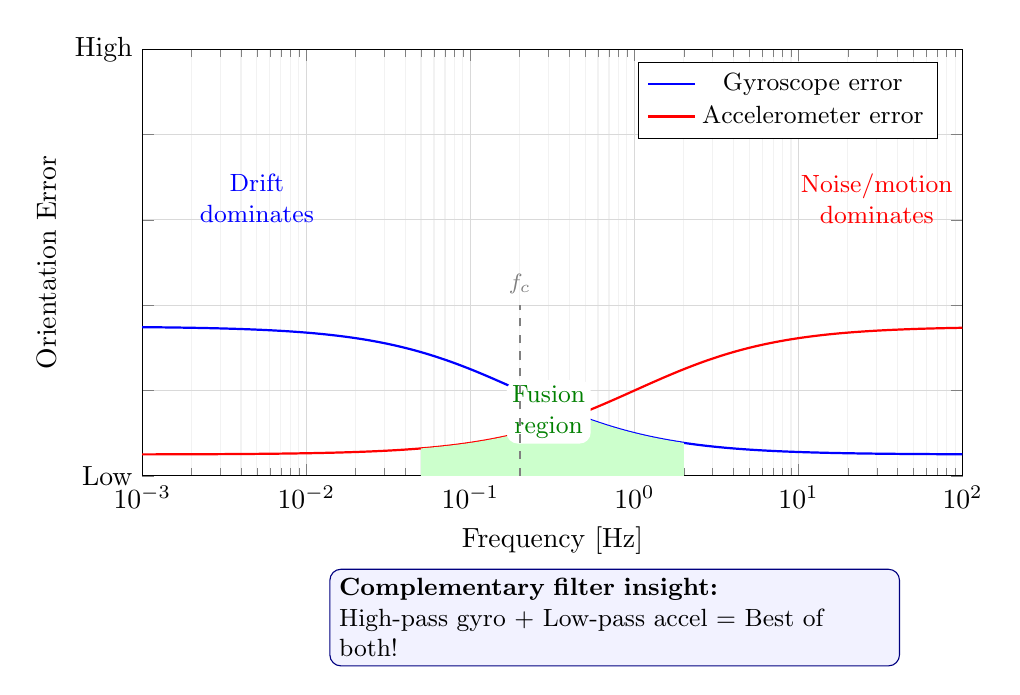
\begin{tikzpicture}
    \begin{semilogxaxis}[
        width=12cm,
        height=7cm,
        xlabel={Frequency [Hz]},
        ylabel={Orientation Error},
        xmin=0.001, xmax=100,
        ymin=0, ymax=10,
        grid=both,
        grid style={gray!30},
        minor grid style={gray!10},
        legend pos=north east,
        legend style={font=\small},
        ytick={0,2,4,6,8,10},
        yticklabels={Low,,,,, High},
    ]
        % Gyroscope error: high at low frequencies (drift), low at high frequencies
        \addplot[thick, blue, domain=0.001:100, samples=200]
            {3/(1 + 5*x) + 0.5};
        \addlegendentry{Gyroscope error}

        % Accelerometer error: low at low frequencies, high at high frequencies
        \addplot[thick, red, domain=0.001:100, samples=200]
            {0.5 + 3*x/(1 + x)};
        \addlegendentry{Accelerometer error}

        % Fusion region (shaded)
        \addplot[fill=green!20, draw=none, domain=0.05:2, samples=50]
            {min(3/(1 + 5*x) + 0.5, 0.5 + 3*x/(1 + x))} \closedcycle;

        % Annotations
        \node[blue, font=\small, align=center] at (axis cs:0.005,6.5)
            {Drift\\dominates};
        \node[red, font=\small, align=center] at (axis cs:30,6.5)
            {Noise/motion\\dominates};
        \node[green!50!black, font=\small, align=center, fill=white,
              rounded corners, inner sep=2pt] at (axis cs:0.3,1.5)
            {Fusion\\region};

        % Crossover frequency marker
        \draw[dashed, gray, thick] (axis cs:0.2,0) -- (axis cs:0.2,4);
        \node[font=\footnotesize, gray] at (axis cs:0.2,4.5) {$f_c$};
    \end{semilogxaxis}

    % Key insight box
    \node[draw=blue!50!black, fill=blue!5, rounded corners,
          font=\small, align=left, text width=7cm]
        at (6,-1.8) {
        \textbf{Complementary filter insight:}\\
        High-pass gyro + Low-pass accel = Best of both!
    };
\end{tikzpicture}
\caption{Sensor error characteristics in the frequency domain. The gyroscope (blue) has low error at high frequencies but drifts at low frequencies. The accelerometer (red) provides good DC reference but is noisy at high frequencies. The complementary filter exploits this frequency separation.}
\label{fig:sensor-frequency-characteristics}
\end{figure}

\begin{keyidea}[title=The Sensor Fusion Insight]
Each sensor has complementary strengths:
\begin{itemize}
    \item \textbf{Gyroscope}: Accurate in the short term, drifts long term
    \item \textbf{Accelerometer}: Noisy but provides absolute roll/pitch reference
\end{itemize}
The solution: \textbf{fuse} them! Trust the gyroscope for fast changes, trust the accelerometer for the long-term average. This is the complementary filter, which we develop next.
\end{keyidea}

\section{Angular Velocity vs. Euler Angle Rates}
\index{angular velocity!vs. Euler rates}
\index{Euler angles!rate transformation}

The gyroscope measures body angular velocity $\boldsymbol{\omega} = [p, q, r]^T$, but Euler angle rates $[\dot\phi, \dot\theta, \dot\psi]^T$ are often more intuitive for understanding motion. A critical insight is that these are \emph{not} the same quantities, and understanding their relationship is essential for correctly implementing attitude estimation.

\begin{notebox}[title=Rotation Convention]
This derivation uses the \textbf{ZYX (yaw-pitch-roll) intrinsic rotation sequence}, consistent with the Euler angle convention used throughout this course. The rotation from world frame to body frame is: first yaw ($\psi$) about the world $z$-axis, then pitch ($\theta$) about the resulting $y'$-axis, then roll ($\phi$) about the final $x''$-axis (which becomes the body $x$-axis).
\end{notebox}

\subsection{Why Are They Different?}

Using the ZYX convention, each Euler angle rate rotates about a \emph{different} axis:
\begin{itemize}
    \item $\dot\psi$ (yaw rate) rotates about the \textbf{world} $z$-axis
    \item $\dot\theta$ (pitch rate) rotates about the \textbf{intermediate} $y'$-axis (after yaw)
    \item $\dot\phi$ (roll rate) rotates about the \textbf{body} $x''$-axis (after yaw and pitch)
\end{itemize}

In contrast, the gyroscope measures angular velocity components $[p, q, r]^T$ all resolved in the \textbf{current body frame}. These three body axes are generally different from the three Euler rotation axes.

%----------------------------------------------------------------------
% FIGURE: Euler Rotation Axes vs Body Axes
%----------------------------------------------------------------------
\begin{figure}[htbp]
\centering
\begin{tikzpicture}[scale=1.1,
    x={(0.85cm,-0.35cm)}, y={(0.85cm,0.35cm)}, z={(0cm,0.95cm)},
    >=Stealth
]
    % World frame (faint)
    \draw[gray!50, thick, ->] (0,0,0) -- (2.5,0,0) node[right, font=\small] {$x_W$};
    \draw[gray!50, thick, ->] (0,0,0) -- (0,2.5,0) node[above, font=\small] {$y_W$};
    \draw[gray!50, thick, ->] (0,0,0) -- (0,0,2.5) node[above, font=\small] {$z_W$};

    % Yaw axis (world z) - green
    \draw[green!60!black, ultra thick, ->] (0,0,0) -- (0,0,2)
        node[above right, font=\small\bfseries] {$\dot\psi$ axis};

    % Body frame (pitched and rolled) - show tilted
    \begin{scope}[rotate around z=20, rotate around y=25]
        % Body axes
        \draw[blue!70, thick, ->] (0,0,0) -- (2,0,0) node[right, font=\small] {$x_B$};
        \draw[blue!70, thick, ->] (0,0,0) -- (0,2,0) node[above, font=\small] {$y_B$};
        \draw[blue!70, thick, ->] (0,0,0) -- (0,0,2) node[above, font=\small] {$z_B$};

        % Roll axis (body x) - red
        \draw[red!70, ultra thick, ->] (0,0,0) -- (1.8,0,0)
            node[below right, font=\small\bfseries] {$\dot\phi$ axis};
    \end{scope}

    % Intermediate pitch axis (after yaw, before roll) - orange
    \begin{scope}[rotate around z=20]
        \draw[orange!80!black, ultra thick, ->] (0,0,0) -- (0,1.8,0)
            node[above left, font=\small\bfseries] {$\dot\theta$ axis};
    \end{scope}

    % Labels
    \node[font=\footnotesize, text width=4cm, align=left] at (5,0,2) {
        \textcolor{green!60!black}{$\bullet$ Yaw axis: World $z$}\\
        \textcolor{orange!80!black}{$\bullet$ Pitch axis: Intermediate $y'$}\\
        \textcolor{red!70}{$\bullet$ Roll axis: Body $x$}
    };

    \node[font=\footnotesize, text width=4cm, align=left] at (5,0,0) {
        \textcolor{blue!70}{Body frame axes $x_B, y_B, z_B$}\\
        \textcolor{blue!70}{(where gyro measures $p, q, r$)}
    };
\end{tikzpicture}
\caption{The three Euler rotation axes do not coincide with body frame axes except at zero orientation. The gyroscope measures angular velocity components along the blue body axes, but Euler rates describe rotations about three different axes (green, orange, red).}
\label{fig:euler-vs-body-axes}
\end{figure}

\subsection{Deriving the Transformation}

To find the relationship, we express the total angular velocity in the body frame as the sum of contributions from each Euler angle rate.

\textbf{Step 1: Yaw rate contribution.}
The yaw rate $\dot\psi$ produces angular velocity $[0, 0, \dot\psi]^T$ in the world frame. To express this in the body frame, we must rotate through the full Euler sequence $R_x(\phi) R_y(\theta) R_z(\psi)$:
\begin{equation}
\boldsymbol{\omega}_\psi^B = R_x(\phi) R_y(\theta) \begin{bmatrix} 0 \\ 0 \\ \dot\psi \end{bmatrix}
= \begin{bmatrix} -\sin\theta \\ \sin\phi\cos\theta \\ \cos\phi\cos\theta \end{bmatrix} \dot\psi
\end{equation}

\textbf{Step 2: Pitch rate contribution.}
The pitch rate $\dot\theta$ produces angular velocity $[0, \dot\theta, 0]^T$ in the intermediate frame (after yaw). We only need to rotate through roll:
\begin{equation}
\boldsymbol{\omega}_\theta^B = R_x(\phi) \begin{bmatrix} 0 \\ \dot\theta \\ 0 \end{bmatrix}
= \begin{bmatrix} 0 \\ \cos\phi \\ -\sin\phi \end{bmatrix} \dot\theta
\end{equation}

\textbf{Step 3: Roll rate contribution.}
The roll rate $\dot\phi$ is already about the body $x$-axis:
\begin{equation}
\boldsymbol{\omega}_\phi^B = \begin{bmatrix} \dot\phi \\ 0 \\ 0 \end{bmatrix}
\end{equation}

\textbf{Total body angular velocity:}
\begin{equation}
\boldsymbol{\omega}^B = \boldsymbol{\omega}_\phi^B + \boldsymbol{\omega}_\theta^B + \boldsymbol{\omega}_\psi^B
\end{equation}

Combining terms gives the \textbf{forward transformation}:
\begin{equation}
\boxed{
\begin{bmatrix} p \\ q \\ r \end{bmatrix} =
\underbrace{\begin{bmatrix}
1 & 0 & -\sin\theta \\
0 & \cos\phi & \sin\phi\cos\theta \\
0 & -\sin\phi & \cos\phi\cos\theta
\end{bmatrix}}_{T(\phi, \theta)}
\begin{bmatrix} \dot\phi \\ \dot\theta \\ \dot\psi \end{bmatrix}
}
\label{eq:euler-to-body-rates}
\end{equation}

\subsection{Physical Interpretation}

\begin{keyidea}[title=When Are Body Rates Equal to Euler Rates?]
At level orientation ($\phi = \theta = 0$), the transformation matrix becomes the identity:
\[
T(0, 0) = \begin{bmatrix} 1 & 0 & 0 \\ 0 & 1 & 0 \\ 0 & 0 & 1 \end{bmatrix}
\]
So $p = \dot\phi$, $q = \dot\theta$, $r = \dot\psi$---body rates equal Euler rates! But as the quadrotor tilts, the three Euler rotation axes diverge from the body axes, and the rates differ.
\end{keyidea}

Examining each row of the transformation:
\begin{itemize}
    \item \textbf{Row 1} ($p$): The body roll rate $p$ equals $\dot\phi$ minus a contribution from $\dot\psi$ when pitched ($-\sin\theta \cdot \dot\psi$). When pitched nose-up, yawing produces some body roll.

    \item \textbf{Row 2} ($q$): The body pitch rate $q$ is a mix of $\dot\theta$ and $\dot\psi$, weighted by roll angle. When rolled, yawing produces body pitch.

    \item \textbf{Row 3} ($r$): The body yaw rate $r$ similarly mixes $\dot\theta$ and $\dot\psi$, weighted by roll angle.
\end{itemize}

\subsection{Worked Examples}

\begin{example}[Level Flight]
At $\phi = 0°$, $\theta = 0°$, with Euler rates $[\dot\phi, \dot\theta, \dot\psi] = [10, 5, 20]$ deg/s:
\begin{align}
\begin{bmatrix} p \\ q \\ r \end{bmatrix} &=
\begin{bmatrix} 1 & 0 & 0 \\ 0 & 1 & 0 \\ 0 & 0 & 1 \end{bmatrix}
\begin{bmatrix} 10 \\ 5 \\ 20 \end{bmatrix} =
\begin{bmatrix} 10 \\ 5 \\ 20 \end{bmatrix} \text{ deg/s}
\end{align}
Body rates equal Euler rates when level.
\end{example}

\begin{example}[Pitched Nose-Up 30°]
At $\phi = 0°$, $\theta = 30°$, with the same Euler rates $[\dot\phi, \dot\theta, \dot\psi] = [10, 5, 20]$ deg/s:
\begin{align}
\begin{bmatrix} p \\ q \\ r \end{bmatrix} &=
\begin{bmatrix} 1 & 0 & -0.5 \\ 0 & 1 & 0 \\ 0 & 0 & 0.866 \end{bmatrix}
\begin{bmatrix} 10 \\ 5 \\ 20 \end{bmatrix} =
\begin{bmatrix} 10 - 10 \\ 5 \\ 17.3 \end{bmatrix} =
\begin{bmatrix} 0 \\ 5 \\ 17.3 \end{bmatrix} \text{ deg/s}
\end{align}
The body roll rate $p$ is now zero! The yaw motion ($\dot\psi = 20$ deg/s) about the world vertical axis contributes to roll in the body frame, canceling the explicit roll rate. The body yaw rate is also reduced.
\end{example}

\subsection{The Inverse Transformation}

To convert gyroscope measurements $[p, q, r]^T$ to Euler angle rates, we invert the matrix:
\begin{equation}
\boxed{
\begin{bmatrix} \dot\phi \\ \dot\theta \\ \dot\psi \end{bmatrix} =
\underbrace{\begin{bmatrix}
1 & \sin\phi\tan\theta & \cos\phi\tan\theta \\
0 & \cos\phi & -\sin\phi \\
0 & \sin\phi\sec\theta & \cos\phi\sec\theta
\end{bmatrix}}_{W(\phi, \theta)}
\begin{bmatrix} p \\ q \\ r \end{bmatrix}
}
\label{eq:body-to-euler-rates}
\end{equation}

This matrix $W(\phi, \theta)$ appears in the attitude kinematics: $\dot{\boldsymbol{\Theta}} = W(\boldsymbol{\Theta}) \boldsymbol{\omega}$.

\subsection{The Singularity Problem}

\begin{warningbox}[title=Singularity at Gimbal Lock]
The inverse transformation contains $\tan\theta$ and $\sec\theta = 1/\cos\theta$. At $\theta = \pm 90°$, these terms are undefined:
\begin{center}
\begin{tabular}{ccc}
\toprule
$\theta$ & $\tan\theta$ & $\sec\theta$ \\
\midrule
$80°$ & 5.67 & 5.76 \\
$85°$ & 11.4 & 11.5 \\
$89°$ & 57.3 & 57.3 \\
$89.9°$ & 573 & 573 \\
$90°$ & $\infty$ & $\infty$ \\
\bottomrule
\end{tabular}
\end{center}
This is another manifestation of gimbal lock---the same singularity we encountered in Euler angle representations.
\end{warningbox}

\begin{example}[Singularity Behavior]
Consider a quadrotor at $\theta = 89°$, $\phi = 10°$, with body angular velocity $[p, q, r] = [0, 10, 0]$ deg/s (pure pitch rate in body frame):
\begin{align}
\dot\phi &= 0 + 10 \cdot \sin(10°) \cdot \tan(89°) + 0 = 10 \cdot 0.174 \cdot 57.3 = 99.6 \text{ deg/s} \\
\dot\theta &= 10 \cdot \cos(10°) = 9.85 \text{ deg/s} \\
\dot\psi &= 10 \cdot \sin(10°) \cdot \sec(89°) = 99.6 \text{ deg/s}
\end{align}

A modest body pitch rate of 10 deg/s requires Euler rates of nearly 100 deg/s! As $\theta \to 90°$, the required Euler rates become unbounded. This is why \textbf{you should never integrate Euler rates directly} near gimbal lock.
\end{example}

\subsection{Quaternion Rate Equation}

For quaternions, the relationship between angular velocity and quaternion rate is elegantly simple and singularity-free:
\begin{equation}
\boxed{\dot{\mathbf{q}} = \frac{1}{2} \mathbf{q} \otimes \begin{bmatrix} 0 \\ \boldsymbol{\omega} \end{bmatrix}}
\label{eq:quaternion-rate}
\end{equation}

where $\boldsymbol{\omega} = [p, q, r]^T$ is the body angular velocity (directly from the gyroscope).

\textbf{Advantages of the quaternion formulation}:
\begin{itemize}
    \item \textbf{No singularity}: Works at any orientation, including $\theta = \pm 90°$
    \item \textbf{Direct gyro use}: The gyroscope output $[p, q, r]$ enters directly---no transformation needed
    \item \textbf{No transcendentals}: Only multiplication and addition (faster than $\sin$, $\cos$, $\tan$)
    \item \textbf{Stable integration}: Quaternion normalization is cheap; Euler angle corrections are not
\end{itemize}

\begin{keyidea}[title=Best Practice for Attitude Integration]
\begin{enumerate}
    \item \textbf{Store orientation as a quaternion} internally
    \item \textbf{Integrate using the quaternion rate equation} $\dot{\mathbf{q}} = \frac{1}{2}\mathbf{q} \otimes [0; \boldsymbol{\omega}]$
    \item \textbf{Normalize} the quaternion periodically: $\mathbf{q} \leftarrow \mathbf{q}/\|\mathbf{q}\|$
    \item \textbf{Convert to Euler angles only for display}---never for computation
\end{enumerate}
This approach avoids gimbal lock entirely and is computationally efficient.
\end{keyidea}


\chapter{Sensor Calibration}
\index{calibration}

Sensor fusion algorithms assume calibrated sensor data. Without proper calibration, even the best estimation algorithm will produce poor results. This chapter covers the practical aspects of IMU calibration\index{calibration|textbf} for quadrotor flight controllers.

\section{Why Calibration Matters}

Raw sensor readings from an IMU contain systematic errors that can be corrected through calibration:

\begin{center}
\begin{tabular}{p{3cm}p{4cm}p{5cm}}
\toprule
\textbf{Error Type} & \textbf{Source} & \textbf{Effect if Uncorrected} \\
\midrule
Bias (offset) & Manufacturing tolerances, temperature & Constant drift, attitude offset \\
Scale factor & Sensitivity variation & Incorrect magnitude, gain error \\
Misalignment & Sensor not aligned with PCB & Cross-axis coupling \\
Non-linearity & Sensor physics & Errors at extreme values \\
Noise & Electronics, quantization & Random fluctuations \\
\bottomrule
\end{tabular}
\end{center}

\begin{example}[Impact of Uncalibrated Gyroscope]
A gyroscope with 1°/s bias, integrated over 10 seconds, produces a 10° attitude error. At 500 Hz sampling, this is:
\[
\theta_{error} = b_{gyro} \cdot t = 1°/\text{s} \times 10\text{ s} = 10°
\]

This error accumulates indefinitely. Without calibration (or sensor fusion), the quadrotor would be uncontrollable within seconds.
\end{example}

\section{The Calibration Model}

A calibrated measurement is obtained from the raw reading using:
\[
\mathbf{m}_{calibrated} = \mathbf{S}^{-1} \cdot \mathbf{M}^{-1} \cdot (\mathbf{m}_{raw} - \mathbf{b})
\]

where:
\begin{itemize}
    \item $\mathbf{m}_{raw}$: Raw sensor reading (vector)
    \item $\mathbf{b}$: Bias vector (offset from zero)
    \item $\mathbf{S}$: Scale factor matrix (diagonal for independent axes)
    \item $\mathbf{M}$: Misalignment matrix (accounts for non-orthogonal axes)
\end{itemize}

For most applications, we can simplify to:
\[
m_{calibrated,i} = \frac{m_{raw,i} - b_i}{s_i}
\]

where $b_i$ is the bias and $s_i$ is the scale factor for axis $i$.

\section{Gyroscope Calibration}

\subsection{Bias Estimation (Static Calibration)}

Gyroscope bias is estimated when the sensor is stationary. The true angular velocity is zero, so any reading is pure bias.

\begin{keyidea}[title=Gyroscope Bias Calibration]
\textbf{Procedure}:
\begin{enumerate}
    \item Place the quadrotor on a stable surface
    \item Collect $N$ samples (typically $N = 1000$ at 500 Hz = 2 seconds)
    \item Compute the average: $\hat{b} = \frac{1}{N} \sum_{i=1}^{N} \omega_{raw,i}$
    \item Store $\hat{b}$ for runtime correction
\end{enumerate}

\textbf{Runtime}: Subtract the estimated bias from each reading:
\[
\omega_{calibrated} = \omega_{raw} - \hat{b}
\]
\end{keyidea}

The complete implementation is provided in Listing~\ref{lst:gyro-calib} (Appendix~\ref{app:code-listings}). The key steps are: (1) collect samples while stationary, (2) compute the mean as the bias estimate, and (3) subtract the bias from all subsequent readings.

\subsection{Bias Drift and Temperature}

Gyroscope bias is not constant---it varies with temperature. A typical MEMS gyroscope has:
\[
b(T) = b_0 + \alpha (T - T_0)
\]

where $\alpha$ is the temperature coefficient (typically 0.01--0.05 °/s/°C).

\begin{notebox}[title=Temperature Compensation]
For precise applications:
\begin{enumerate}
    \item Calibrate at multiple temperatures (e.g., 0°C, 25°C, 50°C)
    \item Fit a polynomial: $b(T) = a_0 + a_1 T + a_2 T^2$
    \item At runtime, read temperature and compute $b(T)$
\end{enumerate}

For the Crazyflie, the temperature change during a short flight is small, so constant bias compensation is usually sufficient.
\end{notebox}

\subsection{Online Bias Estimation}

For longer flights, bias can be estimated online when the quadrotor is detected to be stationary (low acceleration, low angular velocity):

See Listing~\ref{lst:gyro-online} (Appendix~\ref{app:code-listings}) for the complete implementation. The algorithm detects stationary periods by checking both angular velocity and acceleration magnitude, then slowly updates the bias estimate using an exponential moving average.

\section{Accelerometer Calibration}

Accelerometer calibration is more involved because we cannot easily create a ``zero acceleration'' reference (gravity is always present).

\subsection{The Six-Position Method}

The standard method uses gravity as a reference. By placing each axis alternately pointing up and down, we measure $\pm g$ on each axis.

\begin{keyidea}[title=Six-Position Accelerometer Calibration]
\textbf{Positions}:
\begin{enumerate}
    \item $+Z$ up: Expected reading $(0, 0, +g)$
    \item $-Z$ up: Expected reading $(0, 0, -g)$
    \item $+X$ up: Expected reading $(+g, 0, 0)$
    \item $-X$ up: Expected reading $(-g, 0, 0)$
    \item $+Y$ up: Expected reading $(0, +g, 0)$
    \item $-Y$ up: Expected reading $(0, -g, 0)$
\end{enumerate}

From each pair of measurements:
\[
b_i = \frac{m_{+} + m_{-}}{2}, \quad s_i = \frac{m_{+} - m_{-}}{2g}
\]
\end{keyidea}

\begin{example}[Accelerometer Calibration Calculation]
For the Z-axis, we measure:
\begin{itemize}
    \item $+Z$ up (quadrotor upside down): raw reading $= -520$
    \item $-Z$ up (quadrotor right-side up): raw reading $= +510$
\end{itemize}

Expected for $g = 9.81$ m/s² with nominal scale 1000 LSB/g:
\[
b_z = \frac{-520 + 510}{2} = -5 \text{ LSB}
\]
\[
s_z = \frac{-520 - 510}{2 \times 9.81} = \frac{-1030}{19.62} = -52.5 \text{ LSB/(m/s²)}
\]

The negative scale indicates the sensor axis is inverted relative to convention.
\end{example}

The complete implementation including data structures and calibration computation is provided in Listing~\ref{lst:accel-sixpos} (Appendix~\ref{app:code-listings}).

\subsection{Simplified Level Calibration}

For applications where only the level orientation matters (typical for quadrotors), a simpler two-position calibration suffices:

See Listing~\ref{lst:accel-level} (Appendix~\ref{app:code-listings}) for the implementation.

\section{Magnetometer Calibration}

Magnetometers are particularly challenging to calibrate because they are affected by:
\begin{itemize}
    \item \textbf{Hard iron}: Constant magnetic fields from nearby ferromagnetic materials
    \item \textbf{Soft iron}: Distortion of the Earth's field by nearby materials
\end{itemize}

\subsection{Hard Iron Calibration}

Hard iron effects create a constant offset. Calibration involves rotating the sensor through all orientations and finding the center of the resulting ellipsoid.

See Listing~\ref{lst:mag-calib} (Appendix~\ref{app:code-listings}) for the implementation.

\begin{warningbox}[title=Magnetometer Limitations on Quadrotors]
On quadrotors, magnetometers are severely affected by:
\begin{itemize}
    \item Motor magnetic fields (varying with throttle)
    \item Battery current loops
    \item Power wires
\end{itemize}

Many flight controllers ignore magnetometer data during high-throttle flight and use GPS heading instead. For the Crazyflie (indoor, no GPS), yaw estimation often relies on gyroscope integration with occasional magnetometer corrections when motors are at low power.
\end{warningbox}

\section{Calibration Storage and Validation}

\subsection{Storing Calibration Parameters}

Calibration parameters should be stored in non-volatile memory (EEPROM or Flash) so they persist across power cycles:

See Listing~\ref{lst:calib-storage} (Appendix~\ref{app:code-listings}) for a complete implementation including magic number validation and CRC integrity checking.

\subsection{Validating Calibration Quality}

After calibration, verify the quality:

See Listing~\ref{lst:calib-validate} (Appendix~\ref{app:code-listings}) for a complete validation implementation that checks:
\begin{itemize}
    \item Gyro bias within reasonable bounds (typically $< 5$ deg/s)
    \item Accelerometer scale factors close to unity (0.9--1.1)
    \item Calibrated accelerometer magnitude close to $g$ when level
\end{itemize}

\section{Calibration Best Practices}

\begin{keyidea}[title=Calibration Guidelines for Quadrotors]
\begin{enumerate}
    \item \textbf{Calibrate on every cold start}: Gyro bias changes with temperature
    \item \textbf{Wait for thermal equilibrium}: Let the sensors warm up (30--60 seconds) before calibration
    \item \textbf{Use a stable surface}: Any vibration or motion corrupts calibration
    \item \textbf{Recalibrate periodically}: Especially after crashes or sensor replacement
    \item \textbf{Validate after calibration}: Check that calibrated values are reasonable
    \item \textbf{Store calibration data}: Save to EEPROM so it persists across power cycles
    \item \textbf{Log calibration values}: Record for debugging and quality tracking
\end{enumerate}
\end{keyidea}

\begin{notebox}[title=Crazyflie Calibration]
The Crazyflie firmware performs automatic gyroscope bias calibration at startup. When you see the LEDs change pattern after power-on, the gyroscope calibration is complete. The quadrotor must be stationary during this time (typically 1--2 seconds).

Accelerometer calibration parameters are stored in EEPROM and can be updated using the Crazyflie client software.
\end{notebox}


\chapter{Orientation Estimation}

%----------------------------------------------------------------------
% FIGURE: Complementary Filter Concept
%----------------------------------------------------------------------
\begin{figure}[htbp]
\centering
\begin{tikzpicture}[
    block/.style={draw, rectangle, minimum height=2.5em, minimum width=3.5em,
                  align=center, rounded corners=2pt},
    sum/.style={draw, circle, minimum size=1.5em, inner sep=0pt},
    >=Stealth
]
    % === Block Diagram (upper part) ===
    % Gyroscope branch
    \node[block, fill=blue!10] (gyro) at (0,2) {$\omega_g$\\(gyro)};
    \node[block, fill=blue!20] (int) at (2.5,2) {$\displaystyle\frac{1}{s}$};
    \node[block, fill=blue!30] (hp) at (5.5,2) {$\displaystyle\frac{\tau s}{\tau s + 1}$\\High-pass};

    % Accelerometer branch
    \node[block, fill=red!10] (accel) at (0,0) {$\theta_a$\\(accel)};
    \node[block, fill=red!30] (lp) at (5.5,0) {$\displaystyle\frac{1}{\tau s + 1}$\\Low-pass};

    % Summing junction and output
    \node[sum] (sum) at (8,1) {$+$};
    \node[block, fill=green!20] (output) at (10.5,1) {$\hat\theta$\\(estimate)};

    % Connections - gyro branch
    \draw[->] (gyro) -- (int) node[midway, above, font=\small] {rate};
    \draw[->] (int) -- (hp) node[midway, above, font=\small] {$\theta_g$};
    \draw[->] (hp) -- (sum.north west);

    % Connections - accel branch
    \draw[->] (accel) -- (lp) node[midway, above, font=\small] {angle};
    \draw[->] (lp) -- (sum.south west);

    % Output
    \draw[->] (sum) -- (output);

    % Annotations
    \node[blue!70!black, font=\footnotesize, align=center] at (5.5,3.2)
        {Trust gyro at\\high frequencies};
    \node[red!70!black, font=\footnotesize, align=center] at (5.5,-1.2)
        {Trust accel at\\low frequencies};
    \node[green!50!black, font=\footnotesize] at (10.5,2)
        {Best of both!};

    % Key relationship box
    \node[draw=gray, fill=gray!10, rounded corners, font=\small,
          align=center] at (2.5,-2.5)
        {Key property: $G(s) + H(s) = 1$\\(complementary)};

    % === Frequency Response Inset ===
    \begin{scope}[shift={(12.5,1)}]
        \draw[->] (-1.5,-1.5) -- (2,-1.5) node[right, font=\tiny] {$\omega$};
        \draw[->] (-1.5,-1.5) -- (-1.5,1.5) node[above, font=\tiny] {$|H|$};

        % Low-pass response (red)
        \draw[thick, red] (-1.3,1) .. controls (0,0.9) and (0.5,0) .. (1.5,-1.2);
        % High-pass response (blue)
        \draw[thick, blue] (-1.3,-1.2) .. controls (0,-0.5) and (0.5,0.5) .. (1.5,1);

        % Crossover
        \draw[dashed, gray] (0,-1.5) -- (0,1) node[above, font=\tiny] {$\frac{1}{\tau}$};

        % Labels
        \node[red, font=\tiny] at (1.8,-0.8) {LP};
        \node[blue, font=\tiny] at (1.8,0.8) {HP};
    \end{scope}
\end{tikzpicture}
\caption{The complementary filter combines high-pass filtered gyroscope data with low-pass filtered accelerometer data. Since $G(s) + H(s) = 1$, the filters are ``complementary'' and cover all frequencies. The inset shows the frequency responses crossing over at $\omega = 1/\tau$.}
\label{fig:complementary-filter-concept}
\end{figure}

\section{The Sensor Fusion Problem}

We now have all the pieces:
\begin{itemize}
    \item \textbf{Gyroscope}: Gives orientation \emph{rates}, excellent short-term, drifts long-term
    \item \textbf{Accelerometer}: Gives absolute roll/pitch, noisy, corrupted during acceleration
\end{itemize}

The goal: combine these to get accurate orientation estimates that are:
\begin{itemize}
    \item Responsive to fast changes (like the gyroscope)
    \item Accurate in the long term (like the accelerometer)
\end{itemize}

\begin{keyidea}[title=Sensor Fusion Strategy]
\begin{itemize}
    \item For \textbf{fast changes} (high frequency): Trust the gyroscope
    \item For \textbf{slow changes/steady state} (low frequency): Trust the accelerometer
\end{itemize}
This naturally suggests filtering: high-pass filter the gyroscope, low-pass filter the accelerometer, and add.
\end{keyidea}

\section{1D Complementary Filter}
\index{complementary filter}

We derive the filter for a single angle (e.g., pitch). The extension to 3D follows.

\subsection{Setup}

Let:
\begin{itemize}
    \item $\theta$: True angle we want to estimate
    \item $\theta_a$: Angle estimate from accelerometer (noisy but unbiased)
    \item $\omega_g$: Angular velocity from gyroscope (accurate rate but with bias)
\end{itemize}

\subsection{Frequency Domain Derivation}

Define a first-order low-pass filter with time constant $\tau$:
\begin{equation}
G(s) = \frac{1}{\tau s + 1}
\end{equation}

The complementary high-pass filter is:
\begin{equation}
H(s) = 1 - G(s) = \frac{\tau s}{\tau s + 1}
\end{equation}

Key property: $G(s) + H(s) = 1$ for all frequencies. They are ``complementary.''

\textbf{The filter}:
\begin{equation}
\hat\theta(s) = G(s) \cdot \theta_a(s) + H(s) \cdot \theta_g(s)
\end{equation}

where $\theta_g(s) = \omega_g(s)/s$ is the integrated gyroscope signal.

\textbf{Intuition}:
\begin{itemize}
    \item At low frequencies ($\omega \ll 1/\tau$): $G \approx 1$, $H \approx 0$ $\Rightarrow$ use accelerometer
    \item At high frequencies ($\omega \gg 1/\tau$): $G \approx 0$, $H \approx 1$ $\Rightarrow$ use gyroscope
    \item At crossover ($\omega = 1/\tau$): Equal contribution from both
\end{itemize}

\subsection{Time Domain Implementation}

Converting to discrete time with sampling period $h$:

\begin{equation}
\boxed{\hat\theta_k = \alpha \cdot (\hat\theta_{k-1} + h \cdot \omega_{g,k}) + (1-\alpha) \cdot \theta_{a,k}}
\end{equation}

where:
\begin{equation}
\alpha = \frac{\tau}{\tau + h}
\end{equation}

%----------------------------------------------------------------------
% FIGURE: Discrete-Time Complementary Filter
%----------------------------------------------------------------------
\begin{figure}[htbp]
\centering
\begin{tikzpicture}[
    block/.style={draw, rectangle, minimum height=2em, minimum width=2.5em,
                  align=center, rounded corners=2pt},
    gain/.style={draw, circle, minimum size=1.8em, inner sep=0pt, font=\small},
    sum/.style={draw, circle, minimum size=1.5em, inner sep=0pt},
    >=Stealth
]
    % Gyroscope branch
    \node[block, fill=blue!15] (gyro) at (0,1.5) {$\omega_{g,k}$};
    \node[gain, fill=blue!25] (h) at (2,1.5) {$h$};
    \node[sum] (sum1) at (4,1.5) {$+$};
    \node[gain, fill=blue!35] (alpha) at (6,1.5) {$\alpha$};

    % Accelerometer branch
    \node[block, fill=red!15] (accel) at (0,-0.5) {$\theta_{a,k}$};
    \node[gain, fill=red!35] (oneminusalpha) at (6,-0.5) {$1{-}\alpha$};

    % Output summing and delay
    \node[sum] (sum2) at (8,0.5) {$+$};
    \node[block, fill=green!20] (output) at (10,0.5) {$\hat\theta_k$};
    \node[block, fill=gray!20] (delay) at (4,-1.8) {$z^{-1}$};

    % Connections - gyro branch
    \draw[->] (gyro) -- (h);
    \draw[->] (h) -- (sum1);
    \draw[->] (sum1) -- (alpha) node[midway, above, font=\scriptsize] {predict};
    \draw[->] (alpha) -- (sum2.north west);

    % Connections - accel branch
    \draw[->] (accel) -- (oneminusalpha);
    \draw[->] (oneminusalpha) -- (sum2.south west);

    % Output and feedback
    \draw[->] (sum2) -- (output);
    \draw[->] (output.east) -- ++(0.5,0) |- (delay.east);
    \draw[->] (delay.west) -| (sum1.south);

    % Labels
    \node[font=\scriptsize] at (4,-1.2) {$\hat\theta_{k-1}$};
    \node[blue!70!black, font=\footnotesize, align=center] at (3,2.8)
        {Predict from gyro\\(short-term trust)};
    \node[red!70!black, font=\footnotesize, align=center] at (3,-1.6)
        {Correct toward accel\\(long-term reference)};

    % Typical values box
    \node[draw=gray, fill=yellow!10, rounded corners, font=\scriptsize,
          align=left, text width=4.5cm] at (10.5,-1.5) {
        \textbf{Typical values:}\\
        At 100 Hz ($h{=}0.01$s), $\tau{=}1$s:\\
        $\alpha = 0.99$ (99\% gyro, 1\% accel)
    };
\end{tikzpicture}
\caption{Discrete-time complementary filter block diagram. Each iteration predicts from the gyroscope (multiply rate by $h$, add to previous estimate), then corrects toward the accelerometer using a weighted average. The parameter $\alpha$ controls the trust balance.}
\label{fig:discrete-complementary-filter}
\end{figure}

\textbf{Intuition}: Each step:
\begin{enumerate}
    \item Predict using gyroscope: $\hat\theta_{predict} = \hat\theta_{k-1} + h \cdot \omega_{g,k}$
    \item Correct toward accelerometer: blend prediction with accelerometer reading
\end{enumerate}

\subsection{Parameter Selection}

The only tuning parameter is $\tau$ (or equivalently $\alpha$):

\begin{center}
\begin{tabular}{lcc}
\toprule
$\tau$ & $\alpha$ & Behavior \\
\midrule
Large (e.g., 2 s) & $\approx 0.99$ & Trust gyro more, slow correction, less noise \\
Small (e.g., 0.2 s) & $\approx 0.95$ & Trust accel more, fast correction, more noise \\
\bottomrule
\end{tabular}
\end{center}

\begin{notebox}[title=Typical Values]
For quadrotors with MEMS IMUs:
\begin{itemize}
    \item $\tau = 0.5$ to $2$ seconds works well
    \item At 100 Hz ($h = 0.01$ s): $\alpha \approx 0.98$ to $0.995$
\end{itemize}
Start with $\alpha = 0.98$ and tune from there.
\end{notebox}

\subsection{Why Does This Work?}

Consider the error sources:
\begin{itemize}
    \item \textbf{Gyroscope bias}: Creates a slowly-growing error (low frequency). The low-pass filter on the accelerometer corrects this.
    \item \textbf{Accelerometer noise}: High frequency. The high-pass filter on the gyroscope ignores this.
    \item \textbf{Accelerations}: Corrupt accelerometer at high frequencies. The high-pass filter on gyroscope handles fast motion.
\end{itemize}

The complementary filter automatically separates these error sources by frequency!

\section{Extension to 3D: The Mahony Filter}
\index{Mahony filter}

The 1D filter extends to 3D using quaternions. The Mahony filter~\cite{mahony2008nonlinear}\index{Mahony filter|textbf} is a widely-used, computationally efficient approach that provides theoretical guarantees on stability.

\subsection{Key Idea}

Instead of filtering angles directly (which has gimbal lock issues), we:
\begin{enumerate}
    \item Represent orientation as a quaternion
    \item Compute an error vector from the accelerometer
    \item Use this error to correct the gyroscope
    \item Integrate the corrected gyroscope to update the quaternion
\end{enumerate}

\subsection{Error Computation}

\textbf{Step 1}: Normalize accelerometer reading (assuming it measures gravity):
\[
\hat{\mathbf{a}} = \frac{\mathbf{a}_{meas}}{\|\mathbf{a}_{meas}\|}
\]

\textbf{Step 2}: Predict gravity direction in body frame from current quaternion:
\[
\hat{\mathbf{g}}_B = \begin{bmatrix}
2(q_1 q_3 - q_0 q_2) \\
2(q_0 q_1 + q_2 q_3) \\
q_0^2 - q_1^2 - q_2^2 + q_3^2
\end{bmatrix}
\]

This is the third column of the rotation matrix $R^T$ (gravity direction in body frame).

\textbf{Step 3}: Compute error as cross product:
\[
\mathbf{e} = \hat{\mathbf{a}} \times \hat{\mathbf{g}}_B
\]

%----------------------------------------------------------------------
% FIGURE: Mahony Filter Error Computation (Cross Product)
%----------------------------------------------------------------------
\begin{figure}[htbp]
\centering
\begin{tikzpicture}[scale=1.2,
    x={(0.866cm,-0.35cm)}, y={(0.866cm,0.35cm)}, z={(0cm,0.9cm)},
    >=Stealth
]
    % Unit sphere (represented as ellipse)
    \draw[gray!40, thick] (0,0,0) circle (2cm);
    \draw[gray!30, dashed] (2,0,0) arc (0:180:2cm and 0.6cm);
    \draw[gray!40] (-2,0,0) arc (180:360:2cm and 0.6cm);

    % Coordinate axes (faint)
    \draw[gray!30, ->] (0,0,0) -- (2.5,0,0);
    \draw[gray!30, ->] (0,0,0) -- (0,2.5,0);
    \draw[gray!30, ->] (0,0,0) -- (0,0,2.5);

    % Measured gravity vector (accelerometer) - red
    \draw[very thick, red, ->] (0,0,0) -- (0.3,0.5,1.7)
        node[above right, font=\small] {$\hat{\mathbf{a}}$};

    % Predicted gravity vector (from quaternion) - blue
    \draw[very thick, blue, ->] (0,0,0) -- (-0.4,0.7,1.6)
        node[above left, font=\small] {$\hat{\mathbf{g}}_B$};

    % Error vector (cross product) - green, perpendicular to both
    \draw[very thick, green!60!black, ->] (0,0,0) -- (1.5,1.2,0.2)
        node[right, font=\small] {$\mathbf{e} = \hat{\mathbf{a}} \times \hat{\mathbf{g}}_B$};

    % Angle arc between vectors
    \draw[thick, orange] (0.12,0.2,0.68) arc (60:75:0.8);
    \node[orange, font=\footnotesize] at (0.5,0.4,1.1) {$\theta_{err}$};

    % Arc showing rotation path
    \draw[dashed, green!60!black, thick] (0.3,0.5,1.7) arc (35:55:2);

    % Key insight box
    \node[draw=green!50!black, fill=green!5, rounded corners,
          font=\footnotesize, align=left, text width=5cm] at (5.5,0,1.5) {
        \textbf{Cross product gives:}\\
        \textbf{Direction:} Axis to rotate around\\
        \textbf{Magnitude:} $\sin(\theta_{err}) \approx \theta_{err}$
    };

    % Labels
    \node[red!70!black, font=\footnotesize, align=center] at (1.5,-1,2) {Measured\\(from accel)};
    \node[blue!70!black, font=\footnotesize, align=center] at (-1.5,-0.5,2) {Predicted\\(from $q$)};

    % Perfect alignment note
    \node[gray, font=\scriptsize, align=center] at (0,-2.5,0)
        {When $\hat{\mathbf{a}} = \hat{\mathbf{g}}_B$: $\mathbf{e} = 0$ (no correction needed)};
\end{tikzpicture}
\caption{Mahony filter error computation using cross product. The measured gravity $\hat{\mathbf{a}}$ (red) and predicted gravity $\hat{\mathbf{g}}_B$ (blue) are both unit vectors. Their cross product $\mathbf{e}$ (green) gives the axis of rotation needed to align them, with magnitude proportional to the angular error.}
\label{fig:mahony-cross-product}
\end{figure}

\textbf{Intuition}: The cross product measures how much the measured and predicted gravity directions differ. If they align, error is zero. If they differ, the error vector points along the axis of rotation needed to align them.

\subsection{PI Correction}

Apply proportional-integral control to correct the gyroscope:
\begin{align}
\mathbf{e}_{int} &\leftarrow \mathbf{e}_{int} + \mathbf{e} \cdot h \\
\boldsymbol{\omega}_{corrected} &= \boldsymbol{\omega}_{gyro} + K_p \mathbf{e} + K_i \mathbf{e}_{int}
\end{align}

\begin{itemize}
    \item $K_p$: Proportional gain. Higher = faster correction but more noise.
    \item $K_i$: Integral gain. Slowly corrects gyroscope bias.
\end{itemize}

\subsection{Quaternion Integration}

Update quaternion using the corrected angular velocity:
\begin{equation}
q_{k+1} = q_k + \frac{h}{2} q_k \otimes \begin{bmatrix} 0 \\ \boldsymbol{\omega}_{corrected} \end{bmatrix}
\end{equation}

Renormalize to maintain unit quaternion:
\begin{equation}
q_{k+1} \leftarrow \frac{q_{k+1}}{\|q_{k+1}\|}
\end{equation}

%----------------------------------------------------------------------
% FIGURE: Mahony Filter Block Diagram
%----------------------------------------------------------------------
\begin{figure}[htbp]
\centering
\begin{tikzpicture}[
    block/.style={draw, rectangle, minimum height=2em, minimum width=2.8em,
                  align=center, rounded corners=2pt, font=\small},
    smallblock/.style={draw, rectangle, minimum height=1.8em, minimum width=2.2em,
                  align=center, rounded corners=2pt, font=\scriptsize},
    gain/.style={draw, circle, minimum size=1.5em, inner sep=0pt, font=\scriptsize},
    sum/.style={draw, circle, minimum size=1.3em, inner sep=0pt, font=\scriptsize},
    >=Stealth,
    scale=0.95, transform shape
]
    % === INPUTS (left side) ===
    \node[block, fill=blue!15] (gyro) at (0,0) {$\boldsymbol{\omega}_{gyro}$};
    \node[block, fill=red!15] (accel) at (0,3) {$\mathbf{a}_{meas}$};

    % === ACCELEROMETER BRANCH (top) ===
    \node[smallblock, fill=red!25] (norm) at (2.5,3) {Normalize};
    \draw[->, red!70!black] (accel) -- (norm);

    % === ERROR COMPUTATION ===
    \node[smallblock, fill=green!25] (cross) at (5,2) {$\times$\\(cross)};
    \node[smallblock, fill=gray!20] (grav) at (2.5,1) {$\hat{\mathbf{g}}_B$\\from $q$};

    \draw[->, red!70!black] (norm) -| (cross.north) node[pos=0.7, above, font=\scriptsize] {$\hat{\mathbf{a}}$};
    \draw[->, gray] (grav) -| (cross.south);

    % === PI CONTROLLER ===
    \node[gain, fill=green!30] (kp) at (7,2.5) {$K_p$};
    \node[smallblock, fill=green!20] (int) at (7,1) {$\int$};
    \node[gain, fill=green!30] (ki) at (8.5,1) {$K_i$};
    \node[sum] (sumpi) at (9.5,2) {$+$};

    \draw[->, green!60!black] (cross) -- ++(1,0) |- (kp);
    \draw[->, green!60!black] (cross) -- ++(1,0) |- (int);
    \draw[->, green!60!black] (int) -- (ki);
    \draw[->, green!60!black] (kp) -| (sumpi);
    \draw[->, green!60!black] (ki) -| (sumpi);

    % === GYRO CORRECTION ===
    \node[sum] (sumgyro) at (11,0) {$+$};
    \draw[->, blue!70!black] (gyro) -- (sumgyro) node[midway, below, font=\scriptsize] {};
    \draw[->, green!60!black] (sumpi) |- (sumgyro);

    % === QUATERNION INTEGRATION ===
    \node[smallblock, fill=purple!20] (qdot) at (13,0) {$\dot{q} = \frac{1}{2}q \otimes$\\$[0;\boldsymbol{\omega}]$};
    \node[smallblock, fill=purple!25] (qint) at (15.5,0) {$\int$};
    \node[smallblock, fill=purple!30] (qnorm) at (17.5,0) {Norm};

    \draw[->] (sumgyro) -- (qdot) node[midway, above, font=\scriptsize] {$\boldsymbol{\omega}_{corr}$};
    \draw[->] (qdot) -- (qint);
    \draw[->] (qint) -- (qnorm);

    % === OUTPUT ===
    \node[block, fill=purple!15] (output) at (19.5,0) {$q$};
    \draw[->] (qnorm) -- (output);

    % === FEEDBACK LOOP ===
    \draw[->] (output.south) -- ++(0,-1) -| (grav.south);
    \draw[->] (output.south) -- ++(0,-1) -| (13,-1) -- (13,-0.5);

    % === LABELS ===
    \node[blue!70!black, font=\scriptsize] at (0,-0.8) {Gyroscope};
    \node[red!70!black, font=\scriptsize] at (0,3.7) {Accelerometer};
    \node[purple!70!black, font=\scriptsize] at (19.5,0.8) {Output};

    % Color legend
    \node[font=\tiny, align=left] at (5,-1.8) {
        \textcolor{red!70!black}{Red: Accel path} \quad
        \textcolor{blue!70!black}{Blue: Gyro path} \quad
        \textcolor{green!60!black}{Green: Correction} \quad
        \textcolor{purple!70!black}{Purple: Quaternion}
    };

    % Error label
    \node[green!60!black, font=\scriptsize] at (6,2) {$\mathbf{e}$};
\end{tikzpicture}
\caption{Complete Mahony filter block diagram. The accelerometer provides a gravity reference (red path), which is compared to the predicted gravity from the quaternion estimate. The cross product error drives a PI controller (green path) that corrects the gyroscope. The corrected angular velocity integrates the quaternion (purple path), which feeds back for the next iteration.}
\label{fig:mahony-block-diagram}
\end{figure}

\subsection{Complete Algorithm}

The complete Mahony filter implementation is provided in Listing~\ref{lst:mahony-filter} (Appendix~\ref{app:code-listings}). The algorithm performs the following steps each iteration:
\begin{enumerate}
    \item Normalize accelerometer reading to unit vector
    \item Compute predicted gravity direction from current quaternion
    \item Calculate cross-product error between measured and predicted gravity
    \item Apply PI correction to gyroscope readings
    \item Integrate quaternion using corrected angular velocity
    \item Renormalize quaternion to maintain unit magnitude
\end{enumerate}

\subsection{Tuning}

\begin{center}
\begin{tabular}{lll}
\toprule
\textbf{Parameter} & \textbf{Effect} & \textbf{Typical Range} \\
\midrule
$K_p$ & Speed of convergence, noise sensitivity & 0.5 -- 2.0 \\
$K_i$ & Gyro bias correction rate & 0.001 -- 0.01 \\
\bottomrule
\end{tabular}
\end{center}

\begin{notebox}[title=Assumptions for Mahony Filter]
The filter assumes:
\begin{enumerate}
    \item Accelerometer measures primarily gravity (body not accelerating violently)
    \item Gyroscope is the primary source of orientation rate information
    \item Sensor biases are slowly varying
\end{enumerate}
During aggressive maneuvers, consider temporarily increasing $K_p$ or reducing accelerometer trust.
\end{notebox}

\section{Comparison with Kalman Filter}

\begin{center}
\begin{tabular}{lcc}
\toprule
& \textbf{Complementary/Mahony} & \textbf{Extended Kalman Filter} \\
\midrule
Computational cost & Low ($O(1)$ per update) & High (matrix operations) \\
Memory & Minimal & Stores covariance matrix \\
Tuning parameters & 2 ($K_p$, $K_i$) & Many (process/measurement noise) \\
Theoretical basis & Heuristic (frequency separation) & Optimal (for linear Gaussian) \\
Performance & Very good & Excellent \\
\bottomrule
\end{tabular}
\end{center}

\begin{keyidea}[title=When to Use What]
\begin{itemize}
    \item \textbf{Complementary/Mahony filter}: Excellent choice for embedded systems with limited computation. Used in many commercial drones.
    \item \textbf{Extended Kalman Filter}: Preferred when fusing additional sensors (GPS, barometer, vision) or when optimal estimation is required.
\end{itemize}
For this course, the Mahony filter is sufficient and provides excellent intuition about sensor fusion. For readers who want a deeper understanding of optimal estimation, the next chapter develops the Kalman filter from first principles.
\end{keyidea}

%======================================================================
% CHAPTER: Optimal State Estimation
%======================================================================
\chapter{Optimal State Estimation}
\label{ch:kalman-filter}
\index{Kalman filter}

The Mahony filter provides excellent attitude estimates with minimal computation. But what makes it work? Is there a principled way to derive such filters? And how do we extend sensor fusion when we add GPS, barometers, or other sensors?

This chapter develops the \textbf{Kalman filter}~\cite{kalman1960new}---the optimal state estimator for linear systems with Gaussian noise. We then extend it to nonlinear systems via the \textbf{Extended Kalman Filter (EKF)}, which is widely used in aerospace, robotics, and autonomous vehicles. Along the way, we'll discover that the Mahony filter is closely related to the steady-state Kalman filter, providing theoretical justification for its excellent performance. For a comprehensive treatment of Kalman filtering, see Brown and Hwang~\cite{brown2012introduction}.

\section{Why Go Beyond Mahony?}

The Mahony filter works well for attitude estimation, but it has limitations:

\begin{itemize}
    \item \textbf{Fixed sensor fusion structure}: The filter assumes a specific combination of gyroscope and accelerometer. Adding new sensors (GPS, magnetometer, barometer) requires redesigning the filter.

    \item \textbf{No uncertainty quantification}: The Mahony filter provides a point estimate $\hat{q}$ but no measure of confidence. We don't know if our estimate is accurate to 1° or 10°.

    \item \textbf{Heuristic tuning}: The gains $K_p$ and $K_i$ are tuned empirically. There's no systematic way to choose them based on sensor specifications.

    \item \textbf{Suboptimal for varying conditions}: The fixed gains cannot adapt when sensor noise characteristics change (e.g., accelerometer becomes unreliable during aggressive maneuvers).
\end{itemize}

The Kalman filter addresses all these limitations by providing:
\begin{itemize}
    \item A \textbf{modular framework} where adding sensors only requires specifying their measurement equations
    \item \textbf{Uncertainty tracking} via the covariance matrix $P$
    \item \textbf{Optimal gains} computed automatically from sensor noise specifications
    \item \textbf{Adaptive weighting} that automatically trusts sensors less when they become unreliable
\end{itemize}

\section{Probability Foundations}
\label{sec:probability-foundations}

The Kalman filter is fundamentally a probabilistic algorithm. Before deriving it, we need to establish the necessary probability concepts.

\subsection{Random Variables and Expectation}

A \textbf{random variable} $X$ is a variable whose value is determined by a random process. We characterize it by its probability distribution.

\begin{definition}[Expected Value]
The \textbf{expected value} (or mean) of a random variable $X$ is:
\[
\mathbb{E}[X] = \mu_X = \int_{-\infty}^{\infty} x \, p(x) \, dx
\]
where $p(x)$ is the probability density function (PDF).
\end{definition}

\textbf{Intuition}: The expected value is the ``center of mass'' of the probability distribution---the average value we'd observe over many samples.

\begin{definition}[Variance]
The \textbf{variance} measures the spread of a random variable around its mean:
\[
\text{Var}(X) = \sigma_X^2 = \mathbb{E}[(X - \mu_X)^2] = \mathbb{E}[X^2] - \mu_X^2
\]
The \textbf{standard deviation} $\sigma_X = \sqrt{\text{Var}(X)}$ has the same units as $X$.
\end{definition}

\textbf{Intuition}: Variance quantifies uncertainty. A gyroscope with $\sigma = 0.01$ rad/s is more precise than one with $\sigma = 0.1$ rad/s.

\subsection{Gaussian Distribution}

The \textbf{Gaussian} (or normal) distribution is central to Kalman filtering because:
\begin{enumerate}
    \item Many physical noise sources are approximately Gaussian (Central Limit Theorem)
    \item Gaussian distributions remain Gaussian under linear transformations
    \item The math works out elegantly (closed-form solutions)
\end{enumerate}

\begin{definition}[Gaussian Distribution]
A random variable $X$ is \textbf{Gaussian} with mean $\mu$ and variance $\sigma^2$, written $X \sim \mathcal{N}(\mu, \sigma^2)$, if its PDF is:
\[
p(x) = \frac{1}{\sqrt{2\pi\sigma^2}} \exp\left(-\frac{(x-\mu)^2}{2\sigma^2}\right)
\]
\end{definition}

\begin{center}
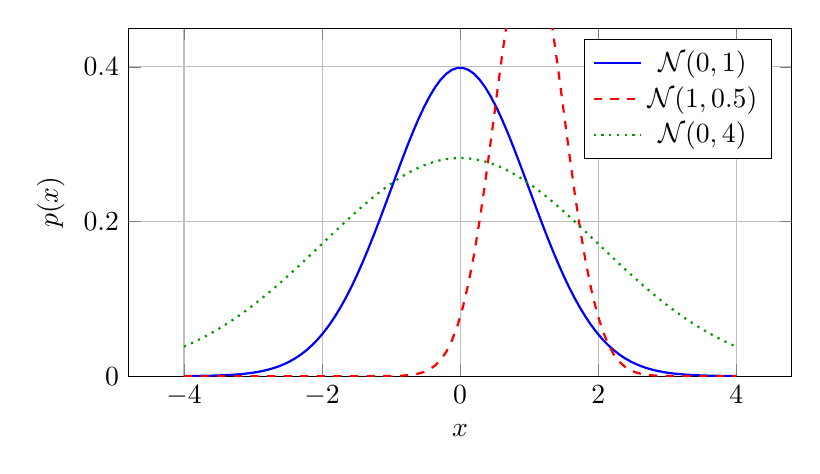
\begin{tikzpicture}
    \begin{axis}[
        width=10cm, height=6cm,
        xlabel={$x$},
        ylabel={$p(x)$},
        domain=-4:4,
        samples=100,
        ymin=0, ymax=0.45,
        legend pos=north east,
        grid=major,
    ]
    \addplot[blue, thick] {exp(-x^2/2)/sqrt(2*pi)};
    \addlegendentry{$\mathcal{N}(0, 1)$}
    \addplot[red, thick, dashed] {exp(-(x-1)^2/0.5)/sqrt(pi)};
    \addlegendentry{$\mathcal{N}(1, 0.5)$}
    \addplot[green!60!black, thick, dotted] {exp(-x^2/8)/sqrt(4*pi)};
    \addlegendentry{$\mathcal{N}(0, 4)$}
    \end{axis}
\end{tikzpicture}
\end{center}

\subsection{Random Vectors and Covariance}

For state estimation, we work with \textbf{random vectors}---vectors whose elements are random variables.

\begin{definition}[Random Vector]
A random vector $\mathbf{x} \in \mathbb{R}^n$ has:
\begin{itemize}
    \item \textbf{Mean vector}: $\boldsymbol{\mu} = \mathbb{E}[\mathbf{x}] = [\mathbb{E}[x_1], \ldots, \mathbb{E}[x_n]]^T$
    \item \textbf{Covariance matrix}: $\mathbf{P} = \mathbb{E}[(\mathbf{x} - \boldsymbol{\mu})(\mathbf{x} - \boldsymbol{\mu})^T]$
\end{itemize}
\end{definition}

The covariance matrix $\mathbf{P}$ is an $n \times n$ symmetric positive semi-definite matrix:
\[
\mathbf{P} = \begin{bmatrix}
\text{Var}(x_1) & \text{Cov}(x_1, x_2) & \cdots & \text{Cov}(x_1, x_n) \\
\text{Cov}(x_2, x_1) & \text{Var}(x_2) & \cdots & \text{Cov}(x_2, x_n) \\
\vdots & \vdots & \ddots & \vdots \\
\text{Cov}(x_n, x_1) & \text{Cov}(x_n, x_2) & \cdots & \text{Var}(x_n)
\end{bmatrix}
\]

where $\text{Cov}(x_i, x_j) = \mathbb{E}[(x_i - \mu_i)(x_j - \mu_j)]$.

\textbf{Interpretation}:
\begin{itemize}
    \item \textbf{Diagonal elements} $P_{ii} = \text{Var}(x_i)$: uncertainty in each state
    \item \textbf{Off-diagonal elements} $P_{ij} = \text{Cov}(x_i, x_j)$: correlation between states
\end{itemize}

\begin{example}[Attitude Estimation Covariance]
For attitude represented as Euler angles $\mathbf{x} = [\phi, \theta, \psi]^T$, a covariance matrix might be:
\[
\mathbf{P} = \begin{bmatrix}
0.01 & 0.002 & 0 \\
0.002 & 0.01 & 0 \\
0 & 0 & 0.04
\end{bmatrix} \text{ rad}^2
\]
This indicates:
\begin{itemize}
    \item Roll and pitch uncertainty: $\sigma_\phi = \sigma_\theta = 0.1$ rad $\approx 5.7°$
    \item Yaw uncertainty: $\sigma_\psi = 0.2$ rad $\approx 11.5°$ (larger because magnetometer is noisy)
    \item Roll-pitch correlation: slightly positive (tilting forward often couples with roll)
    \item No yaw-roll/pitch correlation: yaw errors are independent
\end{itemize}
\end{example}

\subsection{Linear Transformations of Gaussians}

A key property that makes Kalman filtering tractable:

\begin{theorem}[Linear Transformation of Gaussians]
If $\mathbf{x} \sim \mathcal{N}(\boldsymbol{\mu}, \mathbf{P})$ and $\mathbf{y} = \mathbf{A}\mathbf{x} + \mathbf{b}$, then:
\[
\mathbf{y} \sim \mathcal{N}(\mathbf{A}\boldsymbol{\mu} + \mathbf{b}, \mathbf{A}\mathbf{P}\mathbf{A}^T)
\]
\end{theorem}

\textbf{Proof sketch}: The mean transforms linearly: $\mathbb{E}[\mathbf{y}] = \mathbf{A}\mathbb{E}[\mathbf{x}] + \mathbf{b}$. For covariance:
\begin{align*}
\text{Cov}(\mathbf{y}) &= \mathbb{E}[(\mathbf{y} - \mathbb{E}[\mathbf{y}])(\mathbf{y} - \mathbb{E}[\mathbf{y}])^T] \\
&= \mathbb{E}[\mathbf{A}(\mathbf{x} - \boldsymbol{\mu})(\mathbf{x} - \boldsymbol{\mu})^T\mathbf{A}^T] \\
&= \mathbf{A}\mathbb{E}[(\mathbf{x} - \boldsymbol{\mu})(\mathbf{x} - \boldsymbol{\mu})^T]\mathbf{A}^T = \mathbf{A}\mathbf{P}\mathbf{A}^T
\end{align*}

\begin{keyidea}[title=Why This Matters]
This theorem is the foundation of Kalman filtering:
\begin{itemize}
    \item \textbf{Prediction step}: State evolves via $\mathbf{x}_{k+1} = \mathbf{A}\mathbf{x}_k + \ldots$, so covariance transforms as $\mathbf{P}_{k+1} = \mathbf{A}\mathbf{P}_k\mathbf{A}^T + \ldots$
    \item \textbf{Measurement}: Observation is $\mathbf{y} = \mathbf{C}\mathbf{x} + \ldots$, so predicted measurement covariance is $\mathbf{C}\mathbf{P}\mathbf{C}^T + \ldots$
\end{itemize}
Gaussian distributions remain Gaussian through all linear operations, enabling closed-form optimal estimation.
\end{keyidea}

\subsection{Conditional Gaussians and Bayes' Theorem}

When we receive a measurement, we want to update our belief about the state. This is formalized by Bayes' theorem.

\begin{theorem}[Bayes' Theorem]
\[
p(\mathbf{x} | \mathbf{y}) = \frac{p(\mathbf{y} | \mathbf{x}) \, p(\mathbf{x})}{p(\mathbf{y})}
\]
where:
\begin{itemize}
    \item $p(\mathbf{x})$: \textbf{prior}---our belief about $\mathbf{x}$ before seeing $\mathbf{y}$
    \item $p(\mathbf{y} | \mathbf{x})$: \textbf{likelihood}---probability of observing $\mathbf{y}$ given $\mathbf{x}$
    \item $p(\mathbf{x} | \mathbf{y})$: \textbf{posterior}---our updated belief after seeing $\mathbf{y}$
\end{itemize}
\end{theorem}

For jointly Gaussian variables, the posterior has a beautiful closed form:

\begin{theorem}[Gaussian Conditioning]
\label{thm:gaussian-conditioning}
If $\mathbf{x}$ and $\mathbf{y}$ are jointly Gaussian:
\[
\begin{bmatrix} \mathbf{x} \\ \mathbf{y} \end{bmatrix} \sim \mathcal{N}\left(
\begin{bmatrix} \boldsymbol{\mu}_x \\ \boldsymbol{\mu}_y \end{bmatrix},
\begin{bmatrix} \mathbf{P}_{xx} & \mathbf{P}_{xy} \\ \mathbf{P}_{yx} & \mathbf{P}_{yy} \end{bmatrix}
\right)
\]
then the conditional distribution $\mathbf{x} | \mathbf{y}$ is also Gaussian:
\[
\mathbf{x} | \mathbf{y} \sim \mathcal{N}\left(\boldsymbol{\mu}_x + \mathbf{P}_{xy}\mathbf{P}_{yy}^{-1}(\mathbf{y} - \boldsymbol{\mu}_y), \; \mathbf{P}_{xx} - \mathbf{P}_{xy}\mathbf{P}_{yy}^{-1}\mathbf{P}_{yx}\right)
\]
\end{theorem}

\textbf{Interpretation}:
\begin{itemize}
    \item The posterior mean is the prior mean plus a correction term
    \item The correction is proportional to the ``surprise'' $(\mathbf{y} - \boldsymbol{\mu}_y)$---how much the measurement differs from expectation
    \item The posterior covariance is always smaller than the prior (measurements reduce uncertainty)
    \item The matrix $\mathbf{K} = \mathbf{P}_{xy}\mathbf{P}_{yy}^{-1}$ is the \textbf{Kalman gain}
\end{itemize}

\section{The Linear Kalman Filter}
\label{sec:linear-kalman}

We now derive the Kalman filter for linear systems. This provides the foundation for understanding the Extended Kalman Filter used in attitude estimation.

\subsection{Problem Setup}

Consider a discrete-time linear system:

\begin{align}
\mathbf{x}_{k+1} &= \mathbf{A}\mathbf{x}_k + \mathbf{B}\mathbf{u}_k + \mathbf{w}_k & \text{(process model)} \label{eq:kf-process} \\
\mathbf{y}_k &= \mathbf{C}\mathbf{x}_k + \mathbf{v}_k & \text{(measurement model)} \label{eq:kf-measurement}
\end{align}

where:
\begin{itemize}
    \item $\mathbf{x}_k \in \mathbb{R}^n$: state vector (unknown)
    \item $\mathbf{u}_k \in \mathbb{R}^m$: control input (known)
    \item $\mathbf{y}_k \in \mathbb{R}^p$: measurement (observed)
    \item $\mathbf{w}_k \sim \mathcal{N}(\mathbf{0}, \mathbf{Q})$: process noise
    \item $\mathbf{v}_k \sim \mathcal{N}(\mathbf{0}, \mathbf{R})$: measurement noise
\end{itemize}

The matrices $\mathbf{Q}$ and $\mathbf{R}$ are the \textbf{process noise covariance} and \textbf{measurement noise covariance}, respectively.

\begin{example}[1D Attitude Estimation]
\label{ex:1d-kalman}
Consider estimating pitch angle $\theta$ from a gyroscope (measures $\dot{\theta}$) and accelerometer (measures $\theta$ directly, with noise):

\textbf{State}: $x = \theta$ (pitch angle)

\textbf{Process model}: $\theta_{k+1} = \theta_k + h \cdot \omega_k + w_k$

where $\omega_k$ is gyroscope measurement (treated as input $u_k$) and $w_k \sim \mathcal{N}(0, Q)$ captures gyroscope noise/bias.

\textbf{Measurement model}: $y_k = \theta_k + v_k$

where $y_k = \arctan(a_x / a_z)$ from accelerometer and $v_k \sim \mathcal{N}(0, R)$ is accelerometer noise.

In matrix form: $A = 1$, $B = h$, $C = 1$.
\end{example}

\subsection{The Kalman Filter Algorithm}

The Kalman filter alternates between two steps:

\begin{enumerate}
    \item \textbf{Predict}: Use the process model to predict the state at the next time step
    \item \textbf{Update}: Incorporate the measurement to correct the prediction
\end{enumerate}

\begin{tcolorbox}[colback=blue!5!white, colframe=blue!75!black, title=Kalman Filter Algorithm]
\textbf{Initialize}: $\hat{\mathbf{x}}_{0|0} = \mathbb{E}[\mathbf{x}_0]$, $\mathbf{P}_{0|0} = \text{Cov}(\mathbf{x}_0)$

\textbf{For each time step $k$}:

\textit{Predict (time update)}:
\begin{align}
\hat{\mathbf{x}}_{k+1|k} &= \mathbf{A}\hat{\mathbf{x}}_{k|k} + \mathbf{B}\mathbf{u}_k \label{eq:kf-predict-state} \\
\mathbf{P}_{k+1|k} &= \mathbf{A}\mathbf{P}_{k|k}\mathbf{A}^T + \mathbf{Q} \label{eq:kf-predict-cov}
\end{align}

\textit{Update (measurement update)}:
\begin{align}
\mathbf{K}_{k+1} &= \mathbf{P}_{k+1|k}\mathbf{C}^T(\mathbf{C}\mathbf{P}_{k+1|k}\mathbf{C}^T + \mathbf{R})^{-1} \label{eq:kf-gain} \\
\hat{\mathbf{x}}_{k+1|k+1} &= \hat{\mathbf{x}}_{k+1|k} + \mathbf{K}_{k+1}(\mathbf{y}_{k+1} - \mathbf{C}\hat{\mathbf{x}}_{k+1|k}) \label{eq:kf-update-state} \\
\mathbf{P}_{k+1|k+1} &= (\mathbf{I} - \mathbf{K}_{k+1}\mathbf{C})\mathbf{P}_{k+1|k} \label{eq:kf-update-cov}
\end{align}
\end{tcolorbox}

\textbf{Notation}: $\hat{\mathbf{x}}_{k|j}$ denotes the estimate of $\mathbf{x}_k$ given measurements up to time $j$:
\begin{itemize}
    \item $\hat{\mathbf{x}}_{k|k-1}$: predicted estimate (before measurement at time $k$)
    \item $\hat{\mathbf{x}}_{k|k}$: filtered estimate (after measurement at time $k$)
\end{itemize}

\subsection{Understanding the Kalman Gain}

The Kalman gain $\mathbf{K}$ determines how much to trust the measurement versus the prediction:

\[
\mathbf{K} = \mathbf{P}_{k|k-1}\mathbf{C}^T(\mathbf{C}\mathbf{P}_{k|k-1}\mathbf{C}^T + \mathbf{R})^{-1}
\]

\textbf{Extreme cases}:

\begin{itemize}
    \item \textbf{Perfect measurement} ($\mathbf{R} \to \mathbf{0}$): $\mathbf{K} \to \mathbf{C}^{-1}$ (if $\mathbf{C}$ is invertible)

    The estimate jumps directly to the measurement: $\hat{\mathbf{x}}_{k|k} \to \mathbf{C}^{-1}\mathbf{y}_k$

    \item \textbf{Useless measurement} ($\mathbf{R} \to \infty$): $\mathbf{K} \to \mathbf{0}$

    The measurement is ignored: $\hat{\mathbf{x}}_{k|k} \to \hat{\mathbf{x}}_{k|k-1}$

    \item \textbf{Very uncertain prediction} ($\mathbf{P}_{k|k-1} \to \infty$): $\mathbf{K} \to \mathbf{C}^{-1}$

    Trust the measurement completely

    \item \textbf{Very certain prediction} ($\mathbf{P}_{k|k-1} \to \mathbf{0}$): $\mathbf{K} \to \mathbf{0}$

    Ignore the measurement, trust the prediction
\end{itemize}

\begin{keyidea}[title=Kalman Gain Intuition]
The Kalman gain automatically balances trust between prediction and measurement:
\[
\text{Kalman gain} \propto \frac{\text{prediction uncertainty}}{\text{prediction uncertainty} + \text{measurement uncertainty}}
\]
When we're uncertain about our prediction, we trust the measurement more. When the measurement is noisy, we trust our prediction more.
\end{keyidea}

\subsection{Scalar Example: 1D Attitude Filter}

Continuing Example~\ref{ex:1d-kalman}, let's trace through the Kalman filter for pitch estimation.

\textbf{Parameters}:
\begin{itemize}
    \item Sample time: $h = 0.01$ s (100 Hz)
    \item Process noise: $Q = (0.01)^2$ rad$^2$ (gyro drift/noise)
    \item Measurement noise: $R = (0.1)^2$ rad$^2$ (accelerometer noise)
    \item Initial estimate: $\hat{\theta}_0 = 0$, $P_0 = (0.5)^2$ rad$^2$
\end{itemize}

\textbf{Scalar Kalman filter equations}:
\begin{align*}
\text{Predict}: \quad \hat{\theta}_{k|k-1} &= \hat{\theta}_{k-1|k-1} + h \cdot \omega_k \\
P_{k|k-1} &= P_{k-1|k-1} + Q \\[0.5em]
\text{Update}: \quad K_k &= \frac{P_{k|k-1}}{P_{k|k-1} + R} \\
\hat{\theta}_{k|k} &= \hat{\theta}_{k|k-1} + K_k(\theta_{accel,k} - \hat{\theta}_{k|k-1}) \\
P_{k|k} &= (1 - K_k) P_{k|k-1}
\end{align*}

\textbf{Steady-state analysis}: After many iterations, $P$ converges to a constant value. Setting $P_{k|k} = P_{k-1|k-1} = P_{ss}$:
\begin{align*}
P_{ss} + Q &= P_{predict} \\
P_{ss} &= (1 - K_{ss}) P_{predict} = (1 - K_{ss})(P_{ss} + Q)
\end{align*}

Solving: $K_{ss} = \frac{P_{ss} + Q}{P_{ss} + Q + R}$, which gives:
\[
K_{ss} = \frac{-R + \sqrt{R^2 + 4QR + 4Q^2}}{2(Q + R)} \approx \frac{\sqrt{Q}}{\sqrt{Q} + \sqrt{R}} \text{ for small } Q
\]

With our parameters: $K_{ss} \approx 0.09$.

\begin{keyidea}[title=Connection to Complementary Filter]
The steady-state Kalman filter for 1D attitude is equivalent to the complementary filter!

Kalman update: $\hat{\theta}_k = \hat{\theta}_{k|k-1} + K_{ss}(\theta_{accel} - \hat{\theta}_{k|k-1})$

Rewriting: $\hat{\theta}_k = (1 - K_{ss})\hat{\theta}_{k|k-1} + K_{ss} \cdot \theta_{accel}$

This matches the complementary filter $\hat{\theta}_k = \alpha \cdot \hat{\theta}_{gyro} + (1-\alpha) \cdot \theta_{accel}$ with $\alpha = 1 - K_{ss}$.

The complementary filter parameter $\alpha$ corresponds to the steady-state Kalman gain, which the Kalman filter derives automatically from the noise covariances $Q$ and $R$.
\end{keyidea}

\subsection{Optimality of the Kalman Filter}

\begin{theorem}[Kalman Filter Optimality]
For linear systems with Gaussian noise, the Kalman filter provides the \textbf{minimum variance unbiased estimate}:
\[
\hat{\mathbf{x}}_{k|k} = \arg\min_{\hat{\mathbf{x}}} \mathbb{E}\left[\|\mathbf{x}_k - \hat{\mathbf{x}}\|^2 \,|\, \mathbf{y}_{1:k}\right]
\]
where $\mathbf{y}_{1:k} = \{\mathbf{y}_1, \ldots, \mathbf{y}_k\}$ is all measurements up to time $k$.
\end{theorem}

\textbf{Proof sketch}:
\begin{enumerate}
    \item By Theorem~\ref{thm:gaussian-conditioning}, the posterior $p(\mathbf{x}_k | \mathbf{y}_{1:k})$ is Gaussian
    \item For a Gaussian, the mean equals the mode equals the minimum-variance estimate
    \item The Kalman filter recursively computes this posterior mean
\end{enumerate}

\begin{notebox}[title=When is the Kalman Filter Optimal?]
The Kalman filter is optimal \textbf{only} when:
\begin{itemize}
    \item The system is \textbf{linear} (equations \eqref{eq:kf-process}--\eqref{eq:kf-measurement})
    \item Noise is \textbf{Gaussian} with known covariances $\mathbf{Q}$, $\mathbf{R}$
    \item Initial state is \textbf{Gaussian} with known mean and covariance
\end{itemize}
For nonlinear systems (like attitude estimation with quaternions), the Extended Kalman Filter provides an approximation that is no longer guaranteed optimal.
\end{notebox}

\section{The Extended Kalman Filter}
\label{sec:ekf}

Attitude estimation involves nonlinear equations:
\begin{itemize}
    \item Quaternion kinematics: $\dot{\mathbf{q}} = \frac{1}{2}\mathbf{q} \otimes \boldsymbol{\omega}$
    \item Accelerometer measurement: $\mathbf{a} = \mathbf{R}(\mathbf{q})^T \mathbf{g}$
\end{itemize}

The \textbf{Extended Kalman Filter (EKF)} handles nonlinear systems by linearizing around the current estimate at each time step.

\subsection{Nonlinear System Model}

Consider the general nonlinear system:
\begin{align}
\mathbf{x}_{k+1} &= f(\mathbf{x}_k, \mathbf{u}_k) + \mathbf{w}_k \label{eq:ekf-process} \\
\mathbf{y}_k &= h(\mathbf{x}_k) + \mathbf{v}_k \label{eq:ekf-measurement}
\end{align}

where $f(\cdot)$ is the nonlinear process model and $h(\cdot)$ is the nonlinear measurement function.

\subsection{Linearization via Jacobians}

The EKF linearizes these functions around the current estimate using first-order Taylor expansion:
\begin{align*}
f(\mathbf{x}_k, \mathbf{u}_k) &\approx f(\hat{\mathbf{x}}_{k|k}, \mathbf{u}_k) + \mathbf{F}_k(\mathbf{x}_k - \hat{\mathbf{x}}_{k|k}) \\
h(\mathbf{x}_k) &\approx h(\hat{\mathbf{x}}_{k|k-1}) + \mathbf{H}_k(\mathbf{x}_k - \hat{\mathbf{x}}_{k|k-1})
\end{align*}

where the \textbf{Jacobian matrices} are:
\[
\mathbf{F}_k = \frac{\partial f}{\partial \mathbf{x}}\bigg|_{\hat{\mathbf{x}}_{k|k}}, \qquad
\mathbf{H}_k = \frac{\partial h}{\partial \mathbf{x}}\bigg|_{\hat{\mathbf{x}}_{k|k-1}}
\]

\subsection{EKF Algorithm}

\begin{tcolorbox}[colback=blue!5!white, colframe=blue!75!black, title=Extended Kalman Filter Algorithm]
\textbf{Initialize}: $\hat{\mathbf{x}}_{0|0}$, $\mathbf{P}_{0|0}$

\textbf{For each time step $k$}:

\textit{Predict}:
\begin{align}
\hat{\mathbf{x}}_{k+1|k} &= f(\hat{\mathbf{x}}_{k|k}, \mathbf{u}_k) \label{eq:ekf-predict-state} \\
\mathbf{F}_k &= \frac{\partial f}{\partial \mathbf{x}}\bigg|_{\hat{\mathbf{x}}_{k|k}} \\
\mathbf{P}_{k+1|k} &= \mathbf{F}_k\mathbf{P}_{k|k}\mathbf{F}_k^T + \mathbf{Q} \label{eq:ekf-predict-cov}
\end{align}

\textit{Update}:
\begin{align}
\mathbf{H}_{k+1} &= \frac{\partial h}{\partial \mathbf{x}}\bigg|_{\hat{\mathbf{x}}_{k+1|k}} \\
\mathbf{K}_{k+1} &= \mathbf{P}_{k+1|k}\mathbf{H}_{k+1}^T(\mathbf{H}_{k+1}\mathbf{P}_{k+1|k}\mathbf{H}_{k+1}^T + \mathbf{R})^{-1} \label{eq:ekf-gain} \\
\hat{\mathbf{x}}_{k+1|k+1} &= \hat{\mathbf{x}}_{k+1|k} + \mathbf{K}_{k+1}(\mathbf{y}_{k+1} - h(\hat{\mathbf{x}}_{k+1|k})) \label{eq:ekf-update-state} \\
\mathbf{P}_{k+1|k+1} &= (\mathbf{I} - \mathbf{K}_{k+1}\mathbf{H}_{k+1})\mathbf{P}_{k+1|k} \label{eq:ekf-update-cov}
\end{align}
\end{tcolorbox}

The key differences from the linear Kalman filter:
\begin{enumerate}
    \item State prediction uses the \textbf{nonlinear} function $f(\cdot)$, not $\mathbf{A}\hat{\mathbf{x}}$
    \item Measurement prediction uses $h(\hat{\mathbf{x}})$, not $\mathbf{C}\hat{\mathbf{x}}$
    \item Jacobians $\mathbf{F}_k$ and $\mathbf{H}_k$ must be recomputed at each time step
    \item Covariance propagation uses the Jacobians (linearized model)
\end{enumerate}

\subsection{EKF Limitations}

\begin{warningbox}[title=EKF is Not Optimal]
Unlike the linear Kalman filter, the EKF is \textbf{not} optimal:
\begin{itemize}
    \item Linearization introduces errors, especially for highly nonlinear systems
    \item The posterior is approximated as Gaussian, which may not be accurate
    \item The computed covariance $\mathbf{P}$ may not reflect true uncertainty
\end{itemize}

The EKF can \textbf{diverge} (estimates become increasingly wrong) if:
\begin{itemize}
    \item Initial estimate is far from truth (linearization invalid)
    \item System is highly nonlinear
    \item Noise covariances $\mathbf{Q}$, $\mathbf{R}$ are poorly specified
\end{itemize}
\end{warningbox}

\section{Attitude EKF Implementation}
\label{sec:attitude-ekf}

We now develop a complete EKF for attitude estimation using quaternions, suitable for implementation on the Crazyflie.

\subsection{State Representation}

We use the quaternion $\mathbf{q} = [q_0, q_1, q_2, q_3]^T$ as the state, where $q_0$ is the scalar part. The quaternion must satisfy the unit norm constraint $\|\mathbf{q}\| = 1$.

\textbf{State vector}: $\mathbf{x} = \mathbf{q} \in \mathbb{R}^4$

\textbf{Note}: Some implementations use a 3-element ``error state'' representation to avoid the constraint. We use the full quaternion for clarity, with explicit renormalization.

\subsection{Process Model}

The quaternion evolves according to the kinematic equation:
\[
\mathbf{q}_{k+1} = \mathbf{q}_k + \frac{h}{2}\mathbf{q}_k \otimes \begin{bmatrix} 0 \\ \boldsymbol{\omega}_k \end{bmatrix}
\]

where $\boldsymbol{\omega}_k = [p_k, q_k, r_k]^T$ is the angular velocity from the gyroscope.

This can be written as a matrix operation:
\[
\mathbf{q}_{k+1} = \left(\mathbf{I}_4 + \frac{h}{2}\boldsymbol{\Omega}(\boldsymbol{\omega}_k)\right)\mathbf{q}_k
\]

where $\boldsymbol{\Omega}(\boldsymbol{\omega})$ is the $4 \times 4$ matrix:
\[
\boldsymbol{\Omega}(\boldsymbol{\omega}) = \begin{bmatrix}
0 & -p & -q & -r \\
p & 0 & r & -q \\
q & -r & 0 & p \\
r & q & -p & 0
\end{bmatrix}
\]

\textbf{Process model}: $f(\mathbf{q}, \boldsymbol{\omega}) = \left(\mathbf{I}_4 + \frac{h}{2}\boldsymbol{\Omega}(\boldsymbol{\omega})\right)\mathbf{q}$

\textbf{Jacobian}: Since the model is linear in $\mathbf{q}$:
\[
\mathbf{F} = \frac{\partial f}{\partial \mathbf{q}} = \mathbf{I}_4 + \frac{h}{2}\boldsymbol{\Omega}(\boldsymbol{\omega})
\]

\subsection{Measurement Model}

The accelerometer measures the gravity vector in the body frame:
\[
\mathbf{a}_{meas} = \mathbf{R}(\mathbf{q})^T \mathbf{g} + \mathbf{v}
\]

where $\mathbf{g} = [0, 0, g]^T$ (in NED frame) and $\mathbf{R}(\mathbf{q})$ is the rotation matrix corresponding to quaternion $\mathbf{q}$.

The predicted gravity direction in body frame is:
\[
h(\mathbf{q}) = \mathbf{R}(\mathbf{q})^T \begin{bmatrix} 0 \\ 0 \\ g \end{bmatrix} = g \begin{bmatrix}
2(q_1 q_3 - q_0 q_2) \\
2(q_0 q_1 + q_2 q_3) \\
q_0^2 - q_1^2 - q_2^2 + q_3^2
\end{bmatrix}
\]

\textbf{Measurement Jacobian}:
\[
\mathbf{H} = \frac{\partial h}{\partial \mathbf{q}} = 2g \begin{bmatrix}
-q_2 & q_3 & -q_0 & q_1 \\
q_1 & q_0 & q_3 & q_2 \\
q_0 & -q_1 & -q_2 & q_3
\end{bmatrix}
\]

\subsection{Noise Covariance Matrices}

\textbf{Process noise} $\mathbf{Q}$: Represents gyroscope noise and bias drift.
\[
\mathbf{Q} = \sigma_\omega^2 h^2 \mathbf{I}_4
\]
where $\sigma_\omega$ is the gyroscope noise density (rad/s/$\sqrt{\text{Hz}}$).

Typical value for MEMS gyroscope: $\sigma_\omega \approx 0.01$ rad/s, giving $Q_{ii} \approx 10^{-8}$ for $h = 0.01$ s.

\textbf{Measurement noise} $\mathbf{R}$: Represents accelerometer noise.
\[
\mathbf{R} = \sigma_a^2 \mathbf{I}_3
\]
where $\sigma_a$ is the accelerometer noise in m/s² (or equivalently, the angular uncertainty in rad when measuring gravity direction).

Typical value: $\sigma_a \approx 0.5$ m/s², giving $R_{ii} \approx 0.25$ (m/s²)².

\subsection{Complete Algorithm}

The complete attitude EKF implementation is provided in Listing~\ref{lst:attitude-ekf} (Appendix~\ref{app:code-listings}). The code includes:
\begin{itemize}
    \item Data structure with quaternion state and covariance matrices
    \item Initialization with identity quaternion and diagonal covariances
    \item Prediction step using the $\boldsymbol{\Omega}$ matrix from gyroscope readings
    \item Update step using accelerometer measurement of gravity direction
    \item Proper normalization after both prediction and update
\end{itemize}

\subsection{Tuning Guidelines}

\begin{center}
\begin{tabular}{lll}
\toprule
\textbf{Parameter} & \textbf{Effect of Increasing} & \textbf{Typical Range} \\
\midrule
$\mathbf{Q}$ (process noise) & Trust measurements more & $10^{-8}$ to $10^{-4}$ \\
$\mathbf{R}$ (measurement noise) & Trust prediction more & $10^{-2}$ to $10^{1}$ \\
\bottomrule
\end{tabular}
\end{center}

\textbf{Tuning procedure}:
\begin{enumerate}
    \item Start with $\mathbf{Q}$ and $\mathbf{R}$ based on sensor datasheets
    \item If estimates are noisy, increase $\mathbf{R}$ (trust accelerometer less)
    \item If estimates drift, decrease $\mathbf{R}$ or increase $\mathbf{Q}$
    \item If estimates are slow to respond, decrease $\mathbf{R}$
\end{enumerate}

\section{Comparison: Mahony vs. EKF}

\begin{center}
\begin{tabular}{lll}
\toprule
\textbf{Aspect} & \textbf{Mahony Filter} & \textbf{Attitude EKF} \\
\midrule
\textbf{Derivation} & Heuristic (frequency separation) & Principled (Bayesian estimation) \\
\textbf{Tuning} & 2 parameters ($K_p$, $K_i$) & 2 matrices ($\mathbf{Q}$, $\mathbf{R}$) \\
\textbf{Computation} & $\sim$50 operations/update & $\sim$500 operations/update \\
\textbf{Memory} & $\sim$20 floats & $\sim$50 floats \\
\textbf{Uncertainty} & Not available & Covariance matrix $\mathbf{P}$ \\
\textbf{Sensor fusion} & Fixed (gyro + accel) & Easily extensible \\
\textbf{Bias estimation} & Integral term & Can add bias states \\
\textbf{Performance} & Excellent & Excellent \\
\bottomrule
\end{tabular}
\end{center}

\begin{keyidea}[title=When to Choose Each Filter]
\textbf{Use Mahony filter when}:
\begin{itemize}
    \item Computational resources are limited
    \item Only gyroscope and accelerometer are available
    \item Simple tuning is preferred
    \item Uncertainty quantification is not needed
\end{itemize}

\textbf{Use EKF when}:
\begin{itemize}
    \item Fusing additional sensors (GPS, magnetometer, barometer, vision)
    \item Uncertainty bounds are required (for planning, fault detection)
    \item Sensor noise characteristics are well-known
    \item Computational resources are adequate
\end{itemize}

For attitude-only estimation with IMU on a small quadrotor like Crazyflie, the Mahony filter is often the better choice due to its simplicity and efficiency.
\end{keyidea}

\section{Extensions and Advanced Topics}

\subsection{Multiplicative EKF (MEKF)}

The standard EKF with quaternion states has a subtle issue: the four quaternion elements are not independent (they must satisfy $\|\mathbf{q}\| = 1$). This leads to a rank-deficient covariance matrix~\cite{markley2003attitude}.

The \textbf{Multiplicative EKF} addresses this by:
\begin{enumerate}
    \item Maintaining a ``reference'' quaternion $\bar{\mathbf{q}}$ (the current estimate)
    \item Estimating a 3-element ``error rotation'' $\boldsymbol{\delta\theta}$
    \item True quaternion: $\mathbf{q} = \delta\mathbf{q}(\boldsymbol{\delta\theta}) \otimes \bar{\mathbf{q}}$
\end{enumerate}

The error state is always small, making linearization more accurate. After each update, the error is ``folded'' into the reference quaternion, and the error state is reset to zero.

\subsection{Unscented Kalman Filter (UKF)}

Instead of linearizing (which can be inaccurate for highly nonlinear systems), the \textbf{UKF}~\cite{julier1997new} propagates carefully chosen ``sigma points'' through the nonlinear functions and reconstructs the Gaussian approximation from these transformed points.

Advantages over EKF:
\begin{itemize}
    \item No Jacobian computation required
    \item More accurate for highly nonlinear systems
    \item Same computational complexity as EKF
\end{itemize}

\subsection{Multi-Sensor Fusion}

The EKF framework easily accommodates additional sensors by adding measurement update steps:

See Listing~\ref{lst:multisensor-ekf} (Appendix~\ref{app:code-listings}) for a multi-sensor EKF structure that demonstrates sequential sensor updates: prediction using gyroscope, then conditional updates from accelerometer (roll/pitch), magnetometer (yaw), GPS (position/velocity), and barometer (altitude).

Each sensor contributes information according to its noise characteristics ($\mathbf{R}$ matrix), and the Kalman gain automatically weights them appropriately.

\chapter{Quadrotor Dynamics}
\index{quadrotor!dynamics}

%----------------------------------------------------------------------
% FIGURE: Chapter Overview - Quadrotor Force/Torque Diagram
%----------------------------------------------------------------------
\begin{figure}[htbp]
\centering
\begin{tikzpicture}[scale=0.9,
    x={(0.75cm,-0.35cm)}, y={(0.75cm,0.35cm)}, z={(0cm,0.85cm)},
    >=Stealth
]
    % Quadrotor body (tilted slightly)
    \coordinate (center) at (0,0,2);

    % Arms
    \draw[thick, gray!70] ($(center)+(-2.5,0,0)$) -- ($(center)+(2.5,0,0)$);
    \draw[thick, gray!70] ($(center)+(0,-2.5,0)$) -- ($(center)+(0,2.5,0)$);

    % Central body
    \fill[gray!30] ($(center)+(-0.5,-0.5,0)$) -- ($(center)+(0.5,-0.5,0)$)
        -- ($(center)+(0.5,0.5,0)$) -- ($(center)+(-0.5,0.5,0)$) -- cycle;

    % Motors with rotation arrows
    % M1 (front) - CW
    \node[motor] (m1) at ($(center)+(2.5,0,0)$) {};
    \draw[->, thick, blue!60] ($(center)+(2.5,0,0.4)$) arc (90:330:0.3);
    \node[font=\scriptsize] at ($(center)+(2.5,0,0.8)$) {M1};

    % M2 (right) - CCW
    \node[motor] (m2) at ($(center)+(0,2.5,0)$) {};
    \draw[->, thick, red!60] ($(center)+(0,2.5,0.4)$) arc (90:-150:0.3);
    \node[font=\scriptsize] at ($(center)+(0,2.5,0.8)$) {M2};

    % M3 (back) - CW
    \node[motor] (m3) at ($(center)+(-2.5,0,0)$) {};
    \draw[->, thick, blue!60] ($(center)+(-2.5,0,0.4)$) arc (90:330:0.3);
    \node[font=\scriptsize] at ($(center)+(-2.5,0,0.8)$) {M3};

    % M4 (left) - CCW
    \node[motor] (m4) at ($(center)+(0,-2.5,0)$) {};
    \draw[->, thick, red!60] ($(center)+(0,-2.5,0.4)$) arc (90:-150:0.3);
    \node[font=\scriptsize] at ($(center)+(0,-2.5,0.8)$) {M4};

    % Thrust vectors (different heights to show unequal thrust)
    \draw[->, very thick, green!60!black] (m1.center) -- ++(0,0,1.8) node[right, font=\scriptsize] {$T_1$};
    \draw[->, very thick, green!60!black] (m2.center) -- ++(0,0,1.3) node[right, font=\scriptsize] {$T_2$};
    \draw[->, very thick, green!60!black] (m3.center) -- ++(0,0,1.2) node[left, font=\scriptsize] {$T_3$};
    \draw[->, very thick, green!60!black] (m4.center) -- ++(0,0,1.5) node[left, font=\scriptsize] {$T_4$};

    % Weight vector
    \draw[->, very thick, purple] (center) -- ++(0,0,-2.5) node[left, font=\scriptsize] {$mg$};

    % Body frame axes
    \draw[xaxisstyle] (center) -- ++(1.5,0,0) node[below, font=\scriptsize] {$x_B$};
    \draw[yaxisstyle] (center) -- ++(0,1.5,0) node[below, font=\scriptsize] {$y_B$};
    \draw[zaxisstyle] (center) -- ++(0,0,-1.2) node[left, font=\scriptsize] {$z_B$};

    % Torque indicators
    % Roll (around x)
    \draw[->, thick, orange, dashed] ($(center)+(1,0.8,0.3)$) arc (45:135:0.6);
    \node[orange, font=\scriptsize] at ($(center)+(1.5,0,0.8)$) {$\tau_\phi$};

    % Pitch (around y)
    \draw[->, thick, cyan, dashed] ($(center)+(0.8,1,0.3)$) arc (45:135:0.6);
    \node[cyan, font=\scriptsize] at ($(center)+(0,1.5,0.8)$) {$\tau_\theta$};

    % Legend
    \node[font=\scriptsize, align=left] at (5,0,0) {
        \textcolor{blue!60}{CW}: M1, M3\\
        \textcolor{red!60}{CCW}: M2, M4
    };
\end{tikzpicture}
\caption{Forces and torques acting on a quadrotor. Each motor produces thrust $T_i$ (green arrows). Differential thrusts create roll ($\tau_\phi$) and pitch ($\tau_\theta$) torques. Motor spin directions (CW/CCW) enable yaw control through reaction torques. Gravity ($mg$) acts downward.}
\label{fig:quadrotor-force-torque}
\end{figure}

\section{Introduction: Why Study Dynamics?}

We've covered:
\begin{itemize}
    \item How to represent orientation (frames, rotations, quaternions)
    \item How to measure/estimate orientation (IMU, complementary filter)
\end{itemize}

Now we ask: \textbf{how does the quadrotor move?} Given motor commands, what happens to position and orientation?

\textbf{Why this matters}:
\begin{itemize}
    \item \textbf{Simulation}: Before flying, test controllers in simulation
    \item \textbf{Control design}: Controllers are designed based on the dynamics model
    \item \textbf{State estimation}: Some estimation algorithms predict future states using dynamics
\end{itemize}

\section{Physical Description}

\subsection{Configurations}

%----------------------------------------------------------------------
% FIGURE: Quadrotor + vs X Configuration
%----------------------------------------------------------------------
\begin{figure}[htbp]
\centering
\begin{tikzpicture}[>=Stealth, scale=0.85]
    % === Plus Configuration (left) ===
    \begin{scope}[shift={(-5,0)}]
        % Arms
        \draw[thick, gray!70] (0,-2) -- (0,2);
        \draw[thick, gray!70] (-2,0) -- (2,0);

        % Central body
        \fill[gray!30] (-0.3,-0.3) rectangle (0.3,0.3);

        % Motors
        \node[motor] (m1p) at (0,2) {};
        \node[motor] (m2p) at (2,0) {};
        \node[motor] (m3p) at (0,-2) {};
        \node[motor] (m4p) at (-2,0) {};

        % Motor labels and rotation
        \node[font=\scriptsize] at (0,2.5) {M1};
        \node[font=\scriptsize] at (2.5,0) {M2};
        \node[font=\scriptsize] at (0,-2.5) {M3};
        \node[font=\scriptsize] at (-2.5,0) {M4};

        % Rotation arrows
        \draw[->, blue!60, thick] (0.3,2) arc (0:270:0.3);
        \draw[->, red!60, thick] (2,0.3) arc (90:-180:0.3);
        \draw[->, blue!60, thick] (0.3,-2) arc (0:270:0.3);
        \draw[->, red!60, thick] (-2,0.3) arc (90:-180:0.3);

        % Axes
        \draw[->, xaxis, thick] (0,0) -- (0,1.3) node[right, font=\scriptsize] {$x_B$};
        \draw[->, yaxis, thick] (0,0) -- (1.3,0) node[above, font=\scriptsize] {$y_B$};

        % Nose marker
        \fill[black] (0,1.7) -- (-0.15,1.4) -- (0.15,1.4) -- cycle;

        % Arm length
        \draw[<->, gray] (0.2,0) -- (0.2,2) node[midway, right, font=\tiny] {$d$};

        % Label
        \node[font=\small\bfseries] at (0,-3.3) {+ Configuration};
        \node[font=\tiny, gray] at (0,-3.8) {Forward along arm};
    \end{scope}

    % === X Configuration (right) ===
    \begin{scope}[shift={(5,0)}]
        % Arms (rotated 45°)
        \draw[thick, gray!70] (-1.4,-1.4) -- (1.4,1.4);
        \draw[thick, gray!70] (-1.4,1.4) -- (1.4,-1.4);

        % Central body
        \fill[gray!30] (-0.3,-0.3) rectangle (0.3,0.3);

        % Motors
        \node[motor] (m1x) at (1.4,1.4) {};
        \node[motor] (m2x) at (1.4,-1.4) {};
        \node[motor] (m3x) at (-1.4,-1.4) {};
        \node[motor] (m4x) at (-1.4,1.4) {};

        % Motor labels
        \node[font=\scriptsize] at (1.9,1.6) {M1};
        \node[font=\scriptsize] at (1.9,-1.6) {M2};
        \node[font=\scriptsize] at (-1.9,-1.6) {M3};
        \node[font=\scriptsize] at (-1.9,1.6) {M4};

        % Rotation arrows
        \draw[->, blue!60, thick] (1.7,1.4) arc (0:270:0.3);
        \draw[->, red!60, thick] (1.4,-1.1) arc (90:-180:0.3);
        \draw[->, blue!60, thick] (-1.1,-1.4) arc (0:270:0.3);
        \draw[->, red!60, thick] (-1.4,1.7) arc (90:-180:0.3);

        % Axes (between arms)
        \draw[->, xaxis, thick] (0,0) -- (0,1.3) node[right, font=\scriptsize] {$x_B$};
        \draw[->, yaxis, thick] (0,0) -- (1.3,0) node[above, font=\scriptsize] {$y_B$};

        % Nose marker (between M1 and M4)
        \fill[black] (0,1.7) -- (-0.15,1.4) -- (0.15,1.4) -- cycle;

        % Label
        \node[font=\small\bfseries] at (0,-3.3) {X Configuration};
        \node[font=\tiny, gray] at (0,-3.8) {Forward between arms};
    \end{scope}

    % Legend
    \node[font=\tiny, align=center] at (0,-3) {
        \textcolor{blue!60}{CW}: M1, M3 \quad
        \textcolor{red!60}{CCW}: M2, M4
    };
\end{tikzpicture}
\caption{Quadrotor configurations viewed from above. Left: Plus (+) configuration with forward direction along one arm. Right: X configuration (45° rotated) with forward direction between arms. Both use alternating CW/CCW motor directions.}
\label{fig:plus-vs-x-config}
\end{figure}

\begin{center}
\begin{tabular}{lcc}
\toprule
& \textbf{+ Configuration} & \textbf{X Configuration} \\
\midrule
Forward direction & Along one arm & Between two arms \\
Mixing equations & Simpler & Rotated 45° \\
Common use & Educational & Commercial \\
\bottomrule
\end{tabular}
\end{center}

We derive dynamics for the + configuration. The X configuration is identical after a 45° rotation of the mixing matrix.

\subsection{Motor Arrangement}

For + configuration with motors $M_1$ (front), $M_2$ (right), $M_3$ (back), $M_4$ (left):
\begin{itemize}
    \item $M_1$ and $M_3$ spin clockwise (CW)
    \item $M_2$ and $M_4$ spin counter-clockwise (CCW)
\end{itemize}

\textbf{Why alternate directions?} Each spinning propeller creates a reaction torque on the body. By having half spin each way, these torques cancel during hover, allowing yaw control through differential speed.

\subsection{Underactuation}

\begin{definition}
A system is \textbf{underactuated} if it has fewer control inputs than degrees of freedom.
\end{definition}

%----------------------------------------------------------------------
% FIGURE: Underactuation - Why Quadrotors Must Tilt to Move
%----------------------------------------------------------------------
\begin{figure}[htbp]
\centering
\begin{tikzpicture}[>=Stealth, scale=0.9]
    % === Panel 1: Hover ===
    \begin{scope}[shift={(-5,0)}]
        % Quadrotor body (level)
        \draw[thick, gray!70] (-1.5,0) -- (1.5,0);
        \fill[gray!40] (-0.3,-0.15) rectangle (0.3,0.15);
        \node[motor, minimum size=5mm] at (-1.5,0) {};
        \node[motor, minimum size=5mm] at (1.5,0) {};

        % Thrust vector
        \draw[->, very thick, green!60!black] (0,0.2) -- (0,2)
            node[right, font=\small] {$T$};

        % Weight vector
        \draw[->, very thick, purple] (0,-0.2) -- (0,-2)
            node[right, font=\small] {$mg$};

        % Equal signs
        \node[font=\scriptsize] at (0.8,1) {$=$};
        \node[font=\scriptsize] at (0.8,-1) {};

        % Label
        \node[font=\small\bfseries] at (0,-3) {Hover};
        \node[font=\tiny, gray, align=center] at (0,-3.6) {$T = mg$\\No horizontal force};
    \end{scope}

    % === Panel 2: Tilted ===
    \begin{scope}[shift={(0,0)}]
        % Quadrotor body (tilted 20°)
        \draw[thick, gray!70, rotate=20] (-1.5,0) -- (1.5,0);
        \fill[gray!40, rotate=20] (-0.3,-0.15) rectangle (0.3,0.15);
        \node[motor, minimum size=5mm, rotate=20] at ({-1.5*cos(20)},{-1.5*sin(20)}) {};
        \node[motor, minimum size=5mm, rotate=20] at ({1.5*cos(20)},{1.5*sin(20)}) {};

        % Thrust vector (perpendicular to body)
        \draw[->, very thick, green!60!black] (0,0.2) -- ({-2*sin(20)},{2*cos(20)})
            node[above left, font=\small] {$T$};

        % Decompose thrust
        \draw[dashed, green!40!black] ({-2*sin(20)},{2*cos(20)}) -- ({-2*sin(20)},0);
        \draw[dashed, green!40!black] ({-2*sin(20)},{2*cos(20)}) -- (0,{2*cos(20)});

        % Components
        \draw[->, thick, blue] (0,0.2) -- (0,{2*cos(20)})
            node[right, font=\scriptsize, pos=0.7] {$T\cos\theta$};
        \draw[->, thick, red] (0,0.2) -- ({-2*sin(20)},0.2)
            node[below, font=\scriptsize] {$T\sin\theta$};

        % Weight
        \draw[->, very thick, purple] (0,-0.2) -- (0,-1.8)
            node[right, font=\small] {$mg$};

        % Angle arc
        \draw[thick] (0,1) arc (90:110:1) node[midway, above, font=\scriptsize] {$\theta$};

        % Label
        \node[font=\small\bfseries] at (0,-3) {Tilted};
        \node[font=\tiny, gray, align=center] at (0,-3.6) {$F_{horiz} = T\sin\theta$\\Accelerates left!};
    \end{scope}

    % === Panel 3: DOF diagram ===
    \begin{scope}[shift={(5.5,0)}]
        % DOF box
        \node[draw, rounded corners, fill=blue!10, minimum width=2.5cm,
              minimum height=1.5cm, align=center, font=\small] at (0,1.5)
            {6 DOF\\$x,y,z,\phi,\theta,\psi$};

        % Inputs box
        \node[draw, rounded corners, fill=orange!10, minimum width=2.5cm,
              minimum height=1.2cm, align=center, font=\small] at (0,-1)
            {4 Inputs\\$\omega_1,\omega_2,\omega_3,\omega_4$};

        % Arrow
        \draw[->, thick] (0,-0.3) -- (0,0.6);

        % Direct control
        \node[font=\tiny, align=left] at (2.5,1.5) {Direct:\\$z,\phi,\theta,\psi$};

        % Indirect control
        \node[font=\tiny, align=left, red!70!black] at (2.5,0.7) {Via tilt:\\$x, y$};

        % Label
        \node[font=\small\bfseries] at (0,-3) {Underactuated};
        \node[font=\tiny, gray, align=center] at (0,-3.6) {6 DOF, 4 inputs\\Must tilt to translate};
    \end{scope}
\end{tikzpicture}
\caption{Quadrotor underactuation explained. Left: In hover, thrust balances gravity with no horizontal force. Center: To accelerate horizontally, the quadrotor must tilt, creating a horizontal thrust component. Right: With 6 degrees of freedom but only 4 control inputs, horizontal position must be controlled indirectly through attitude.}
\label{fig:underactuation}
\end{figure}

\begin{keyidea}[title=Quadrotor Underactuation]
\begin{itemize}
    \item Degrees of freedom: 6 (position $x, y, z$ and orientation $\phi, \theta, \psi$)
    \item Control inputs: 4 (motor speeds $\omega_1, \omega_2, \omega_3, \omega_4$)
\end{itemize}
\textbf{Consequence}: Cannot independently control all 6 DOF. To move horizontally, the quadrotor must first tilt, directing some thrust sideways. This is why attitude control is fundamental to position control.
\end{keyidea}

\section{Forces and Torques}
\index{thrust}\index{torque}

\subsection{Motor Thrust}

\begin{notebox}[title=Assumption: Quasi-Steady Aerodynamics]
We assume propeller thrust and torque are proportional to the square of propeller speed:
\[
T_i = b \cdot \omega_i^2, \quad Q_i = k \cdot \omega_i^2
\]
This is valid when:
\begin{itemize}
    \item Propeller speed changes slowly compared to air response
    \item Free-stream velocity is small (hover or slow flight)
    \item Ground effect is negligible
\end{itemize}
For aggressive maneuvers, these assumptions may break down.
\end{notebox}

Each motor produces thrust proportional to speed squared:
\begin{equation}
T_i = b \cdot \omega_i^2
\end{equation}

where $b$ is the thrust coefficient (determined experimentally or from propeller theory).

Total thrust:
\begin{equation}
T = b(\omega_1^2 + \omega_2^2 + \omega_3^2 + \omega_4^2)
\end{equation}

\subsection{Motor Drag Torque}

Each spinning propeller creates a reaction torque:
\begin{equation}
Q_i = k \cdot \omega_i^2
\end{equation}

where $k$ is the drag coefficient.

\subsection{Body Torques}

\textbf{Roll torque} (about $x_B$): Differential thrust between left and right motors:
\begin{equation}
\tau_\phi = d(T_4 - T_2) = db(\omega_4^2 - \omega_2^2)
\end{equation}

\textbf{Pitch torque} (about $y_B$): Differential thrust between front and back:
\begin{equation}
\tau_\theta = d(T_1 - T_3) = db(\omega_1^2 - \omega_3^2)
\end{equation}

\textbf{Yaw torque} (about $z_B$): Net reaction torque from all motors:
\begin{equation}
\tau_\psi = k(\omega_1^2 + \omega_3^2 - \omega_2^2 - \omega_4^2)
\end{equation}

where $d$ is the arm length from center to motor.

%----------------------------------------------------------------------
% FIGURE: Yaw Torque from Motor Reaction
%----------------------------------------------------------------------
\begin{figure}[htbp]
\centering
\begin{tikzpicture}[>=Stealth, scale=0.9]
    % === Left panel: Single motor physics ===
    \begin{scope}[shift={(-5,0)}]
        % Motor body (side view)
        \fill[gray!40] (-0.3,-1) rectangle (0.3,0);
        \draw[thick] (-0.3,-1) -- (-0.3,0) -- (0.3,0) -- (0.3,-1);

        % Propeller (top view indication)
        \draw[thick, fill=gray!20] (-1.5,0) -- (-0.3,0.1) -- (-0.3,-0.1) -- cycle;
        \draw[thick, fill=gray!20] (1.5,0) -- (0.3,0.1) -- (0.3,-0.1) -- cycle;

        % Propeller rotation (CW when viewed from above)
        \draw[->, thick, blue!60] (0.8,0.5) arc (30:330:0.5)
            node[right, pos=0.5, font=\scriptsize] {spin};

        % Drag torque on propeller (opposes rotation)
        \draw[->, very thick, red] (-0.6,0.8) arc (150:30:0.6)
            node[above, font=\scriptsize, pos=0.5] {$Q_{drag}$};

        % Reaction torque on body
        \draw[->, very thick, green!60!black] (0,-1.5) arc (-90:90:0.4)
            node[right, font=\scriptsize] {$Q_{react}$};

        % Newton's third law annotation
        \node[font=\scriptsize, align=center] at (0,-2.5) {Reaction torque\\on airframe};

        % Label
        \node[font=\small\bfseries] at (0,2) {Single Motor};
    \end{scope}

    % === Right panel: Four motors (top view) ===
    \begin{scope}[shift={(3,0)}]
        % Arms
        \draw[thick, gray!70] (0,-2) -- (0,2);
        \draw[thick, gray!70] (-2,0) -- (2,0);

        % Central body
        \fill[gray!30] (-0.4,-0.4) rectangle (0.4,0.4);

        % Motors
        \node[motor, minimum size=6mm] (m1) at (0,2) {};
        \node[motor, minimum size=6mm] (m2) at (2,0) {};
        \node[motor, minimum size=6mm] (m3) at (0,-2) {};
        \node[motor, minimum size=6mm] (m4) at (-2,0) {};

        % Motor labels
        \node[font=\scriptsize] at (0,2.6) {M1 (CW)};
        \node[font=\scriptsize] at (2.8,0) {M2 (CCW)};
        \node[font=\scriptsize] at (0,-2.6) {M3 (CW)};
        \node[font=\scriptsize] at (-2.8,0) {M4 (CCW)};

        % Reaction torque arrows (opposite to motor spin)
        % CW motors -> CCW reaction on body
        \draw[->, thick, blue!60] (0.3,2) arc (0:-270:0.3);
        \draw[->, thick, blue!60] (0.3,-2) arc (0:-270:0.3);
        % CCW motors -> CW reaction on body
        \draw[->, thick, red!60] (2,0.3) arc (90:360:0.3);
        \draw[->, thick, red!60] (-2,0.3) arc (90:360:0.3);

        % Net yaw torque (example: yaw CW)
        \draw[->, very thick, orange] (0.6,0) arc (0:-300:0.6)
            node[below right, font=\scriptsize, pos=0.4] {$\tau_\psi$};

        % Legend
        \node[font=\tiny, align=left, blue!60] at (4,1.5) {CW spin\\$\rightarrow$ CCW reaction};
        \node[font=\tiny, align=left, red!60] at (4,0.5) {CCW spin\\$\rightarrow$ CW reaction};
    \end{scope}

    % Key insight box
    \node[draw=orange!70!black, fill=orange!5, rounded corners,
          font=\scriptsize, align=center, text width=5cm] at (3,-3.5) {
        \textbf{To yaw CW:} Speed up M2, M4 (CCW motors)\\
        More CW reaction torque $\rightarrow$ body yaws CW
    };
\end{tikzpicture}
\caption{Yaw control via motor reaction torques. Left: Each spinning propeller experiences aerodynamic drag; by Newton's third law, this creates a reaction torque on the airframe. Right: CW and CCW motors create opposite reaction torques. Yaw is controlled by varying the balance between CW and CCW motor speeds.}
\label{fig:yaw-torque}
\end{figure}

\textbf{Intuition}: Yaw is controlled by the \emph{difference in total torque} between CW and CCW motors, not by thrust differences.

\section{Control Allocation (Mixing)}
\index{mixing matrix}\index{control allocation|see{mixing matrix}}

\subsection{The Mixing Matrix}

We want to map desired total thrust $T$ and torques $(\tau_\phi, \tau_\theta, \tau_\psi)$ to motor speed squares:

\begin{equation}
\begin{bmatrix} T \\ \tau_\phi \\ \tau_\theta \\ \tau_\psi \end{bmatrix} =
\underbrace{\begin{bmatrix}
b & b & b & b \\
0 & -db & 0 & db \\
db & 0 & -db & 0 \\
k & -k & k & -k
\end{bmatrix}}_{M}
\begin{bmatrix} \omega_1^2 \\ \omega_2^2 \\ \omega_3^2 \\ \omega_4^2 \end{bmatrix}
\end{equation}

\subsection{Inverse Mixing}

The controller computes desired $(T, \tau_\phi, \tau_\theta, \tau_\psi)$. We need motor speeds:

\begin{equation}
\begin{bmatrix} \omega_1^2 \\ \omega_2^2 \\ \omega_3^2 \\ \omega_4^2 \end{bmatrix} = M^{-1}
\begin{bmatrix} T \\ \tau_\phi \\ \tau_\theta \\ \tau_\psi \end{bmatrix}
\end{equation}

For the + configuration:
\begin{equation}
M^{-1} = \begin{bmatrix}
\frac{1}{4b} & 0 & \frac{1}{2db} & \frac{1}{4k} \\
\frac{1}{4b} & -\frac{1}{2db} & 0 & -\frac{1}{4k} \\
\frac{1}{4b} & 0 & -\frac{1}{2db} & \frac{1}{4k} \\
\frac{1}{4b} & \frac{1}{2db} & 0 & -\frac{1}{4k}
\end{bmatrix}
\end{equation}

\section{Equations of Motion}

\subsection{Translational Dynamics}

Newton's second law in the world frame:
\begin{equation}
m \ddot{\mathbf{r}} = \mathbf{F}_{gravity} + \mathbf{F}_{thrust} + \mathbf{F}_{drag}
\end{equation}

\begin{notebox}[title=Assumptions for Translational Dynamics]
\begin{itemize}
    \item Rigid body (no structural deformation)
    \item Point mass (mass concentrated at COG)
    \item Aerodynamic drag is linear in velocity (valid for low speeds)
    \item No wind
\end{itemize}
\end{notebox}

Expanding:
\begin{equation}
m \begin{bmatrix} \ddot{x} \\ \ddot{y} \\ \ddot{z} \end{bmatrix} =
\begin{bmatrix} 0 \\ 0 \\ mg \end{bmatrix} +
R^W_B \begin{bmatrix} 0 \\ 0 \\ -T \end{bmatrix} -
\begin{bmatrix} A_x \dot{x} \\ A_y \dot{y} \\ A_z \dot{z} \end{bmatrix}
\end{equation}

\textbf{Interpretation}:
\begin{itemize}
    \item Gravity pulls down (positive $z$ in NED)
    \item Thrust is along body $z$-axis (up in body frame, rotated to world by $R^W_B$)
    \item Drag opposes velocity
\end{itemize}

\subsection{Rotational Dynamics}

Euler's equation for a rotating rigid body:
\begin{equation}
\mathbf{J} \dot{\boldsymbol{\omega}} = -\boldsymbol{\omega} \times (\mathbf{J} \boldsymbol{\omega}) + \boldsymbol{\tau}
\end{equation}

\begin{notebox}[title=Assumptions for Rotational Dynamics]
\begin{itemize}
    \item Rigid body with constant inertia matrix $\mathbf{J}$
    \item Principal axes aligned with body axes (diagonal $\mathbf{J}$)
    \item Negligible rotor gyroscopic effects (valid for small, fast rotors)
\end{itemize}
\end{notebox}

For a symmetric quadrotor with $\mathbf{J} = \text{diag}(J_x, J_y, J_z)$:
\begin{align}
J_x \dot{p} &= (J_y - J_z) qr + \tau_\phi \\
J_y \dot{q} &= (J_z - J_x) pr + \tau_\theta \\
J_z \dot{r} &= (J_x - J_y) pq + \tau_\psi
\end{align}

\textbf{Interpretation}: The $(J_y - J_z)qr$ terms are \emph{gyroscopic coupling}---rotation about one axis affects rotation about others. For symmetric quadrotors ($J_x \approx J_y$), this effect is small.

\section{Complete State-Space Model}
\label{sec:state-space-model}

This section presents the complete mathematical model of the quadrotor in state-space form. We carefully define the notation, present both the full nonlinear model and its linearization around hover, and explain the relationship between them.

\subsection{State-Space Notation}

A \textbf{state-space model} represents a dynamical system as a set of first-order differential equations. The general form is:
\begin{equation}
\dot{\mathbf{x}} = f(\mathbf{x}, \mathbf{u}), \quad \mathbf{y} = h(\mathbf{x}, \mathbf{u})
\label{eq:nonlinear-ss}
\end{equation}
where:
\begin{itemize}
    \item $\mathbf{x} \in \mathbb{R}^n$ is the \textbf{state vector}---the minimum set of variables needed to completely describe the system's condition
    \item $\mathbf{u} \in \mathbb{R}^m$ is the \textbf{input vector}---the control signals we can manipulate
    \item $\mathbf{y} \in \mathbb{R}^p$ is the \textbf{output vector}---the quantities we measure or care about
    \item $f: \mathbb{R}^n \times \mathbb{R}^m \to \mathbb{R}^n$ is the \textbf{state transition function}
    \item $h: \mathbb{R}^n \times \mathbb{R}^m \to \mathbb{R}^p$ is the \textbf{output function}
\end{itemize}

For \textbf{linear} systems, these functions are matrix multiplications:
\begin{equation}
\dot{\mathbf{x}} = A\mathbf{x} + B\mathbf{u}, \quad \mathbf{y} = C\mathbf{x} + D\mathbf{u}
\label{eq:linear-ss}
\end{equation}
where $A \in \mathbb{R}^{n \times n}$, $B \in \mathbb{R}^{n \times m}$, $C \in \mathbb{R}^{p \times n}$, $D \in \mathbb{R}^{p \times m}$.

\subsection{State Vector Definition}
\label{sec:state-vector}

The quadrotor's state must capture everything needed to predict its future motion. This requires 12 variables:

\begin{equation}
\mathbf{x} = \begin{bmatrix} \mathbf{p} \\ \boldsymbol{\Theta} \\ \mathbf{v} \\ \boldsymbol{\omega} \end{bmatrix}
= \begin{bmatrix} x \\ y \\ z \\ \phi \\ \theta \\ \psi \\ v_x \\ v_y \\ v_z \\ p \\ q \\ r \end{bmatrix} \in \mathbb{R}^{12}
\label{eq:state-vector}
\end{equation}

\textbf{Component explanation}:
\begin{center}
\begin{tabular}{cllll}
\toprule
\textbf{Index} & \textbf{Symbol} & \textbf{Name} & \textbf{Frame} & \textbf{Units} \\
\midrule
1--3 & $\mathbf{p} = [x, y, z]^T$ & Position & World (NED) & m \\
4--6 & $\boldsymbol{\Theta} = [\phi, \theta, \psi]^T$ & Euler angles (roll, pitch, yaw) & Body-to-World & rad \\
7--9 & $\mathbf{v} = [v_x, v_y, v_z]^T$ & Linear velocity & World (NED) & m/s \\
10--12 & $\boldsymbol{\omega} = [p, q, r]^T$ & Angular velocity & Body & rad/s \\
\bottomrule
\end{tabular}
\end{center}

\begin{notebox}[title=Frame Conventions]
\begin{itemize}
    \item Position $\mathbf{p}$ and velocity $\mathbf{v}$ are expressed in the \textbf{world frame} (NED): $x$ points North, $y$ points East, $z$ points Down
    \item Angular velocity $\boldsymbol{\omega}$ is expressed in the \textbf{body frame}: $p$ is roll rate (about $x_B$), $q$ is pitch rate (about $y_B$), $r$ is yaw rate (about $z_B$)
    \item Euler angles $\boldsymbol{\Theta}$ define the rotation from world to body frame using ZYX convention
\end{itemize}
\end{notebox}

\subsection{Input Vector Definition}

The control inputs are the total thrust and three body-axis torques:
\begin{equation}
\mathbf{u} = \begin{bmatrix} T \\ \tau_\phi \\ \tau_\theta \\ \tau_\psi \end{bmatrix} \in \mathbb{R}^{4}
\label{eq:input-vector}
\end{equation}

where:
\begin{itemize}
    \item $T$ [N]: Total thrust magnitude (sum of all motor thrusts, along body $-z_B$ axis)
    \item $\tau_\phi$ [N$\cdot$m]: Roll torque (about body $x_B$ axis)
    \item $\tau_\theta$ [N$\cdot$m]: Pitch torque (about body $y_B$ axis)
    \item $\tau_\psi$ [N$\cdot$m]: Yaw torque (about body $z_B$ axis)
\end{itemize}

These inputs are computed from motor speeds via the mixing matrix (Section~\ref{sec:control-allocation}).

\subsection{Full Nonlinear State-Space Model}
\label{sec:nonlinear-model}

The complete nonlinear dynamics can be written as $\dot{\mathbf{x}} = f(\mathbf{x}, \mathbf{u})$, which expands to 12 first-order differential equations:

\textbf{Position kinematics} (states 1--3):
\begin{equation}
\dot{\mathbf{p}} = \mathbf{v} \quad \Leftrightarrow \quad
\begin{cases}
\dot{x} = v_x \\
\dot{y} = v_y \\
\dot{z} = v_z
\end{cases}
\label{eq:position-kinematics}
\end{equation}

These are simply kinematic relations: velocity is the time derivative of position.

\textbf{Attitude kinematics} (states 4--6):
\begin{equation}
\dot{\boldsymbol{\Theta}} = W(\boldsymbol{\Theta}) \boldsymbol{\omega} \quad \Leftrightarrow \quad
\begin{cases}
\dot{\phi} = p + (q \sin\phi + r\cos\phi)\tan\theta \\
\dot{\theta} = q\cos\phi - r\sin\phi \\
\dot{\psi} = (q\sin\phi + r\cos\phi)\sec\theta
\end{cases}
\label{eq:attitude-kinematics}
\end{equation}

where $W(\boldsymbol{\Theta})$ is the transformation from body angular velocity to Euler angle rates:
\begin{equation}
W(\boldsymbol{\Theta}) = \begin{bmatrix}
1 & \sin\phi\tan\theta & \cos\phi\tan\theta \\
0 & \cos\phi & -\sin\phi \\
0 & \sin\phi\sec\theta & \cos\phi\sec\theta
\end{bmatrix}
\label{eq:euler-rate-matrix}
\end{equation}

\begin{warningbox}[title=Singularity]
The matrix $W(\boldsymbol{\Theta})$ becomes singular when $\theta = \pm 90°$ (gimbal lock). This is a limitation of the Euler angle representation, not the physical system. For simulation near vertical orientations, use quaternions instead.
\end{warningbox}

\textbf{Translational dynamics} (states 7--9):
\begin{equation}
m\dot{\mathbf{v}} = \mathbf{F}_g + \mathbf{F}_T + \mathbf{F}_D
\label{eq:translational-dynamics}
\end{equation}

Expanding in the world frame (NED):
\begin{equation}
\begin{cases}
\dot{v}_x = -\dfrac{T}{m}(\cos\psi\sin\theta\cos\phi + \sin\psi\sin\phi) - \dfrac{A_x}{m}v_x \\[10pt]
\dot{v}_y = -\dfrac{T}{m}(\sin\psi\sin\theta\cos\phi - \cos\psi\sin\phi) - \dfrac{A_y}{m}v_y \\[10pt]
\dot{v}_z = g - \dfrac{T}{m}\cos\theta\cos\phi - \dfrac{A_z}{m}v_z
\end{cases}
\label{eq:velocity-dynamics}
\end{equation}

where:
\begin{itemize}
    \item The thrust terms come from $R^W_B \cdot [0, 0, -T]^T$ (thrust along body $-z_B$, rotated to world frame)
    \item $A_x, A_y, A_z$ are aerodynamic drag coefficients (typically small for slow flight)
    \item $g = 9.81$ m/s² is gravitational acceleration (positive in NED, since $z$ points down)
\end{itemize}

\textbf{Rotational dynamics} (states 10--12):
\begin{equation}
J\dot{\boldsymbol{\omega}} = -\boldsymbol{\omega} \times (J\boldsymbol{\omega}) + \boldsymbol{\tau}
\label{eq:rotational-dynamics}
\end{equation}

For a symmetric quadrotor with diagonal inertia matrix $J = \text{diag}(J_x, J_y, J_z)$:
\begin{equation}
\begin{cases}
\dot{p} = \dfrac{J_y - J_z}{J_x}qr + \dfrac{\tau_\phi}{J_x} \\[10pt]
\dot{q} = \dfrac{J_z - J_x}{J_y}pr + \dfrac{\tau_\theta}{J_y} \\[10pt]
\dot{r} = \dfrac{J_x - J_y}{J_z}pq + \dfrac{\tau_\psi}{J_z}
\end{cases}
\label{eq:angular-dynamics}
\end{equation}

The terms $(J_y - J_z)qr/J_x$, etc., are \textbf{gyroscopic coupling} terms arising from the cross product $\boldsymbol{\omega} \times (J\boldsymbol{\omega})$.

\subsection{Compact Matrix Form}

The full nonlinear model can be written compactly as:
\begin{equation}
\boxed{
\dot{\mathbf{x}} = f(\mathbf{x}, \mathbf{u}) = \begin{bmatrix}
\mathbf{v} \\
W(\boldsymbol{\Theta})\boldsymbol{\omega} \\
\frac{1}{m}\left( \mathbf{F}_g + R^W_B(\boldsymbol{\Theta})\mathbf{F}_T^B - D\mathbf{v} \right) \\
J^{-1}\left( -\boldsymbol{\omega} \times (J\boldsymbol{\omega}) + \boldsymbol{\tau} \right)
\end{bmatrix}
}
\label{eq:full-nonlinear}
\end{equation}

where:
\begin{itemize}
    \item $\mathbf{F}_g = [0, 0, mg]^T$ (gravity in NED world frame)
    \item $\mathbf{F}_T^B = [0, 0, -T]^T$ (thrust in body frame)
    \item $R^W_B(\boldsymbol{\Theta})$ is the rotation matrix from body to world (function of $\phi, \theta, \psi$)
    \item $D = \text{diag}(A_x, A_y, A_z)$ is the drag matrix
    \item $\boldsymbol{\tau} = [\tau_\phi, \tau_\theta, \tau_\psi]^T$
\end{itemize}

\begin{keyidea}[title=Structure of the Nonlinear Model]
The 12-state model has a clear structure:
\begin{enumerate}
    \item \textbf{Kinematics} (6 equations): Geometric relationships between positions/angles and velocities---no forces involved
    \item \textbf{Dynamics} (6 equations): Newton/Euler equations relating forces/torques to accelerations
\end{enumerate}
The nonlinearities come from:
\begin{itemize}
    \item Trigonometric functions in $W(\boldsymbol{\Theta})$ and $R^W_B(\boldsymbol{\Theta})$
    \item Gyroscopic coupling $\boldsymbol{\omega} \times (J\boldsymbol{\omega})$
    \item Product of thrust $T$ with orientation-dependent direction
\end{itemize}
\end{keyidea}

\section{Linearization Around Hover}
\index{linearization}\index{hover}

The nonlinear model~\eqref{eq:full-nonlinear} is accurate but difficult to analyze and design controllers for. \textbf{Linearization} approximates the nonlinear system by a linear one, valid near a chosen operating point. This enables powerful linear control design techniques.

\subsection{The Linearization Procedure}

Given a nonlinear system $\dot{\mathbf{x}} = f(\mathbf{x}, \mathbf{u})$, linearization proceeds as follows:

\textbf{Step 1: Choose an equilibrium point} $(\mathbf{x}_0, \mathbf{u}_0)$ satisfying $f(\mathbf{x}_0, \mathbf{u}_0) = \mathbf{0}$.

\textbf{Step 2: Define perturbation variables}:
\begin{equation}
\delta\mathbf{x} = \mathbf{x} - \mathbf{x}_0, \quad \delta\mathbf{u} = \mathbf{u} - \mathbf{u}_0
\end{equation}

\textbf{Step 3: Taylor expand} $f$ around $(\mathbf{x}_0, \mathbf{u}_0)$:
\begin{equation}
\dot{\mathbf{x}} = f(\mathbf{x}_0, \mathbf{u}_0) + \frac{\partial f}{\partial \mathbf{x}}\bigg|_0 \delta\mathbf{x} + \frac{\partial f}{\partial \mathbf{u}}\bigg|_0 \delta\mathbf{u} + \text{higher order terms}
\end{equation}

\textbf{Step 4: Neglect higher-order terms} to obtain the linear model:
\begin{equation}
\delta\dot{\mathbf{x}} = A\,\delta\mathbf{x} + B\,\delta\mathbf{u}
\label{eq:linearized-model}
\end{equation}

where the \textbf{Jacobian matrices} are:
\begin{equation}
A = \frac{\partial f}{\partial \mathbf{x}}\bigg|_{(\mathbf{x}_0, \mathbf{u}_0)} \in \mathbb{R}^{12 \times 12}, \quad
B = \frac{\partial f}{\partial \mathbf{u}}\bigg|_{(\mathbf{x}_0, \mathbf{u}_0)} \in \mathbb{R}^{12 \times 4}
\end{equation}

\subsection{Hover Equilibrium Point}

For a quadrotor, the natural equilibrium is \textbf{hover}---stationary flight with level attitude.

\begin{definition}[Hover Equilibrium]
The hover equilibrium $(\mathbf{x}_0, \mathbf{u}_0)$ is defined by:
\begin{align}
\mathbf{x}_0 &= [x_0, y_0, z_0, 0, 0, \psi_0, 0, 0, 0, 0, 0, 0]^T \label{eq:hover-state} \\
\mathbf{u}_0 &= [mg, 0, 0, 0]^T \label{eq:hover-input}
\end{align}
\end{definition}

\textbf{Interpretation}:
\begin{itemize}
    \item \textbf{Position} $(x_0, y_0, z_0)$: Any fixed point in space (the hover location)
    \item \textbf{Attitude} $(\phi_0, \theta_0, \psi_0) = (0, 0, \psi_0)$: Level orientation (roll and pitch zero), heading $\psi_0$ can be arbitrary
    \item \textbf{Velocities}: All zero (stationary)
    \item \textbf{Thrust} $T_0 = mg$: Exactly balances gravity
    \item \textbf{Torques} $\tau_{\phi,0} = \tau_{\theta,0} = \tau_{\psi,0} = 0$: No rotation commanded
\end{itemize}

\textbf{Verification}: Substituting into the nonlinear model~\eqref{eq:full-nonlinear}:
\begin{itemize}
    \item Position: $\dot{\mathbf{p}} = \mathbf{v}_0 = \mathbf{0}$ \checkmark
    \item Attitude: $\dot{\boldsymbol{\Theta}} = W(\boldsymbol{\Theta}_0)\boldsymbol{\omega}_0 = \mathbf{0}$ \checkmark
    \item Velocity: $\dot{\mathbf{v}} = [0, 0, g - T_0\cos(0)\cos(0)/m]^T = [0, 0, g - g]^T = \mathbf{0}$ \checkmark
    \item Angular velocity: $\dot{\boldsymbol{\omega}} = J^{-1}(\mathbf{0} + \mathbf{0}) = \mathbf{0}$ \checkmark
\end{itemize}

\subsection{Small-Perturbation Variables}

We define perturbations from hover:
\begin{equation}
\delta\mathbf{x} = \begin{bmatrix}
\delta x \\ \delta y \\ \delta z \\ \delta\phi \\ \delta\theta \\ \delta\psi \\
\delta v_x \\ \delta v_y \\ \delta v_z \\ \delta p \\ \delta q \\ \delta r
\end{bmatrix}, \quad
\delta\mathbf{u} = \begin{bmatrix}
\delta T \\ \delta\tau_\phi \\ \delta\tau_\theta \\ \delta\tau_\psi
\end{bmatrix}
\label{eq:perturbation-vars}
\end{equation}

where $T = mg + \delta T$ (thrust perturbation from hover thrust).

\textbf{Small-angle approximations} (valid for $|\phi|, |\theta| \ll 1$ radian, say $< 15°$):
\begin{equation}
\sin\alpha \approx \alpha, \quad \cos\alpha \approx 1, \quad \tan\alpha \approx \alpha
\label{eq:small-angle}
\end{equation}

\subsection{Computing the Jacobian Matrices}

Evaluating the partial derivatives at hover (with $\psi_0 = 0$ for simplicity):

\textbf{System matrix $A$} (12 × 12):

The structure of $A$ reflects the physical coupling between states:

\begin{equation}
A = \left[\begin{array}{c|c|c|c}
\mathbf{0}_{3\times3} & \mathbf{0}_{3\times3} & I_{3\times3} & \mathbf{0}_{3\times3} \\
\hline
\mathbf{0}_{3\times3} & \mathbf{0}_{3\times3} & \mathbf{0}_{3\times3} & I_{3\times3} \\
\hline
\mathbf{0}_{3\times3} & A_{v\Theta} & A_{vv} & \mathbf{0}_{3\times3} \\
\hline
\mathbf{0}_{3\times3} & \mathbf{0}_{3\times3} & \mathbf{0}_{3\times3} & \mathbf{0}_{3\times3}
\end{array}\right]
\label{eq:A-matrix-structure}
\end{equation}

where the non-zero blocks are:
\begin{equation}
A_{v\Theta} = \frac{\partial \dot{\mathbf{v}}}{\partial \boldsymbol{\Theta}}\bigg|_0 = \begin{bmatrix}
0 & -g & 0 \\
g & 0 & 0 \\
0 & 0 & 0
\end{bmatrix}, \quad
A_{vv} = -\frac{1}{m}\begin{bmatrix}
A_x & 0 & 0 \\
0 & A_y & 0 \\
0 & 0 & A_z
\end{bmatrix}
\label{eq:A-submatrices}
\end{equation}

\textbf{Physical interpretation of $A$}:
\begin{itemize}
    \item Row 1--3: Position changes with velocity ($\dot{\mathbf{p}} = \mathbf{v}$)
    \item Row 4--6: Euler angles change with angular velocity (at small angles: $\dot{\boldsymbol{\Theta}} \approx \boldsymbol{\omega}$)
    \item Row 7--9: Velocity changes with attitude (tilt causes horizontal acceleration via gravity) and with velocity itself (drag)
    \item Row 10--12: Angular velocity has no linear dependence on state at hover (gyroscopic terms vanish when $\boldsymbol{\omega}_0 = \mathbf{0}$)
\end{itemize}

\textbf{Input matrix $B$} (12 × 4):

\begin{equation}
B = \frac{\partial f}{\partial \mathbf{u}}\bigg|_0 = \begin{bmatrix}
\mathbf{0}_{3\times4} \\
\mathbf{0}_{3\times4} \\
B_v \\
B_\omega
\end{bmatrix}
\label{eq:B-matrix}
\end{equation}

where:
\begin{equation}
B_v = \begin{bmatrix}
0 & 0 & 0 & 0 \\
0 & 0 & 0 & 0 \\
-1/m & 0 & 0 & 0
\end{bmatrix}, \quad
B_\omega = \begin{bmatrix}
0 & 1/J_x & 0 & 0 \\
0 & 0 & 1/J_y & 0 \\
0 & 0 & 0 & 1/J_z
\end{bmatrix}
\label{eq:B-submatrices}
\end{equation}

\textbf{Physical interpretation of $B$}:
\begin{itemize}
    \item Thrust $\delta T$ directly affects vertical acceleration $\dot{v}_z$ (with gain $-1/m$; negative because $+z$ is down in NED)
    \item Torques $\tau_\phi, \tau_\theta, \tau_\psi$ directly affect angular accelerations $\dot{p}, \dot{q}, \dot{r}$
\end{itemize}

\subsection{Full Linearized State-Space Model}

Combining the above, the linearized model is:

\begin{equation}
\boxed{
\delta\dot{\mathbf{x}} = A\,\delta\mathbf{x} + B\,\delta\mathbf{u}
}
\label{eq:linearized-full}
\end{equation}

with explicit matrices (neglecting drag, i.e., $A_x = A_y = A_z = 0$):

\begin{equation}
A = \begin{bmatrix}
0 & 0 & 0 & 0 & 0 & 0 & 1 & 0 & 0 & 0 & 0 & 0 \\
0 & 0 & 0 & 0 & 0 & 0 & 0 & 1 & 0 & 0 & 0 & 0 \\
0 & 0 & 0 & 0 & 0 & 0 & 0 & 0 & 1 & 0 & 0 & 0 \\
0 & 0 & 0 & 0 & 0 & 0 & 0 & 0 & 0 & 1 & 0 & 0 \\
0 & 0 & 0 & 0 & 0 & 0 & 0 & 0 & 0 & 0 & 1 & 0 \\
0 & 0 & 0 & 0 & 0 & 0 & 0 & 0 & 0 & 0 & 0 & 1 \\
0 & 0 & 0 & 0 & -g & 0 & 0 & 0 & 0 & 0 & 0 & 0 \\
0 & 0 & 0 & g & 0 & 0 & 0 & 0 & 0 & 0 & 0 & 0 \\
0 & 0 & 0 & 0 & 0 & 0 & 0 & 0 & 0 & 0 & 0 & 0 \\
0 & 0 & 0 & 0 & 0 & 0 & 0 & 0 & 0 & 0 & 0 & 0 \\
0 & 0 & 0 & 0 & 0 & 0 & 0 & 0 & 0 & 0 & 0 & 0 \\
0 & 0 & 0 & 0 & 0 & 0 & 0 & 0 & 0 & 0 & 0 & 0 \\
\end{bmatrix}
\label{eq:A-explicit}
\end{equation}

\begin{equation}
B = \begin{bmatrix}
0 & 0 & 0 & 0 \\
0 & 0 & 0 & 0 \\
0 & 0 & 0 & 0 \\
0 & 0 & 0 & 0 \\
0 & 0 & 0 & 0 \\
0 & 0 & 0 & 0 \\
0 & 0 & 0 & 0 \\
0 & 0 & 0 & 0 \\
-1/m & 0 & 0 & 0 \\
0 & 1/J_x & 0 & 0 \\
0 & 0 & 1/J_y & 0 \\
0 & 0 & 0 & 1/J_z \\
\end{bmatrix}
\label{eq:B-explicit}
\end{equation}

\subsection{Decoupled Subsystem Interpretation}

A remarkable property of the linearized quadrotor model is that it \textbf{decouples} into independent subsystems:

\textbf{1. Altitude subsystem} (states: $z$, $v_z$; input: $\delta T$):
\begin{equation}
\begin{bmatrix} \delta\dot{z} \\ \delta\dot{v}_z \end{bmatrix} =
\begin{bmatrix} 0 & 1 \\ 0 & 0 \end{bmatrix}
\begin{bmatrix} \delta z \\ \delta v_z \end{bmatrix} +
\begin{bmatrix} 0 \\ -1/m \end{bmatrix} \delta T
\label{eq:altitude-subsystem}
\end{equation}

This is a \textbf{double integrator}: $m\ddot{z} = -\delta T$.

\textbf{2. Longitudinal subsystem} (states: $x$, $\theta$, $v_x$, $q$; input: $\tau_\theta$):
\begin{equation}
\begin{bmatrix} \delta\dot{x} \\ \delta\dot{\theta} \\ \delta\dot{v}_x \\ \delta\dot{q} \end{bmatrix} =
\begin{bmatrix} 0 & 0 & 1 & 0 \\ 0 & 0 & 0 & 1 \\ 0 & -g & 0 & 0 \\ 0 & 0 & 0 & 0 \end{bmatrix}
\begin{bmatrix} \delta x \\ \delta\theta \\ \delta v_x \\ \delta q \end{bmatrix} +
\begin{bmatrix} 0 \\ 0 \\ 0 \\ 1/J_y \end{bmatrix} \tau_\theta
\label{eq:longitudinal-subsystem}
\end{equation}

The key coupling: pitch angle $\theta$ causes horizontal acceleration via gravity ($\dot{v}_x = -g\theta$).

\textbf{3. Lateral subsystem} (states: $y$, $\phi$, $v_y$, $p$; input: $\tau_\phi$):
\begin{equation}
\begin{bmatrix} \delta\dot{y} \\ \delta\dot{\phi} \\ \delta\dot{v}_y \\ \delta\dot{p} \end{bmatrix} =
\begin{bmatrix} 0 & 0 & 1 & 0 \\ 0 & 0 & 0 & 1 \\ 0 & g & 0 & 0 \\ 0 & 0 & 0 & 0 \end{bmatrix}
\begin{bmatrix} \delta y \\ \delta\phi \\ \delta v_y \\ \delta p \end{bmatrix} +
\begin{bmatrix} 0 \\ 0 \\ 0 \\ 1/J_x \end{bmatrix} \tau_\phi
\label{eq:lateral-subsystem}
\end{equation}

Similar structure: roll angle $\phi$ causes lateral acceleration ($\dot{v}_y = g\phi$).

\textbf{4. Yaw subsystem} (states: $\psi$, $r$; input: $\tau_\psi$):
\begin{equation}
\begin{bmatrix} \delta\dot{\psi} \\ \delta\dot{r} \end{bmatrix} =
\begin{bmatrix} 0 & 1 \\ 0 & 0 \end{bmatrix}
\begin{bmatrix} \delta\psi \\ \delta r \end{bmatrix} +
\begin{bmatrix} 0 \\ 1/J_z \end{bmatrix} \tau_\psi
\label{eq:yaw-subsystem}
\end{equation}

Another \textbf{double integrator}: $J_z\ddot{\psi} = \tau_\psi$.

\begin{keyidea}[title=Why Decoupling Matters]
The 12-state system decomposes into four independent subsystems:
\begin{center}
\begin{tabular}{lccc}
\toprule
\textbf{Subsystem} & \textbf{States} & \textbf{Input} & \textbf{Structure} \\
\midrule
Altitude & 2 & $\delta T$ & Double integrator \\
Longitudinal ($x$-$\theta$) & 4 & $\tau_\theta$ & Cascaded double integrators \\
Lateral ($y$-$\phi$) & 4 & $\tau_\phi$ & Cascaded double integrators \\
Yaw & 2 & $\tau_\psi$ & Double integrator \\
\bottomrule
\end{tabular}
\end{center}
This decoupling means we can design four independent controllers, greatly simplifying the control problem.
\end{keyidea}

\subsection{Physical Insight: Tilt-to-Accelerate}

The linearized model reveals a fundamental principle:

\begin{equation}
\boxed{
\ddot{x} \approx -g\theta, \quad \ddot{y} \approx g\phi
}
\label{eq:tilt-accelerate}
\end{equation}

\textbf{To move North} (positive $x$): pitch nose-down ($\theta < 0$), creating a horizontal thrust component.

\textbf{To move East} (positive $y$): roll right ($\phi > 0$), tilting the thrust vector eastward.

This is why quadrotor position control uses a \textbf{cascaded architecture}:
\begin{enumerate}
    \item \textbf{Outer loop} (position controller): Computes desired attitude angles $(\phi_d, \theta_d)$ from position error
    \item \textbf{Inner loop} (attitude controller): Tracks the desired attitude by commanding torques
\end{enumerate}

\subsection{Validity of the Linearized Model}

The linearized model~\eqref{eq:linearized-full} is accurate when:
\begin{itemize}
    \item Roll and pitch angles satisfy $|\phi|, |\theta| < 15°$ (small-angle assumption)
    \item Angular velocities are small ($|p|, |q|, |r| < 1$ rad/s)
    \item Thrust is close to hover ($|T - mg| < 0.3mg$)
\end{itemize}

For aggressive maneuvers violating these assumptions, use the full nonlinear model~\eqref{eq:full-nonlinear} or gain-scheduled linearizations at multiple operating points.

%----------------------------------------------------------------------
% FIGURE: Cascaded Control Architecture
%----------------------------------------------------------------------
\begin{figure}[htbp]
\centering
\begin{tikzpicture}[
    block/.style={draw, rectangle, minimum height=2.2em, minimum width=2.8em,
                  align=center, rounded corners=2pt, font=\small},
    sum/.style={draw, circle, minimum size=1.3em, inner sep=0pt, font=\scriptsize},
    >=Stealth,
    scale=0.85, transform shape
]
    % === Position Control (outer loop - blue) ===
    \node[block, fill=blue!15] (rdes) at (0,0) {$\mathbf{r}_{des}$\\$(x,y,z)$};
    \node[sum] (sumpos) at (2,0) {$-$};
    \node[block, fill=blue!30, minimum width=3.5em] (posctrl) at (4.5,0)
        {Position\\Controller};

    % === Attitude Control (middle loop - green) ===
    \node[sum] (sumatt) at (7,0) {$-$};
    \node[block, fill=green!30, minimum width=3.5em] (attctrl) at (9.5,0)
        {Attitude\\Controller};

    % === Motor Mixing (orange) ===
    \node[block, fill=orange!30] (mix) at (12.5,0) {$M^{-1}$\\Mixing};

    % === Plant (gray) ===
    \node[block, fill=gray!30, minimum width=4em, minimum height=3em] (plant) at (15.5,0)
        {Quadrotor\\Dynamics};

    % Forward path connections
    \draw[->] (rdes) -- (sumpos);
    \draw[->, blue!70!black] (sumpos) -- (posctrl)
        node[midway, above, font=\tiny] {$e_{pos}$};
    \draw[->, blue!70!black] (posctrl) -- (sumatt)
        node[midway, above, font=\tiny] {$\phi_d,\theta_d,T$};
    \draw[->, green!70!black] (sumatt) -- (attctrl)
        node[midway, above, font=\tiny] {$e_{att}$};
    \draw[->, green!70!black] (attctrl) -- (mix)
        node[midway, above, font=\tiny] {$\boldsymbol{\tau}$};
    \draw[->, orange!70!black] (mix) -- (plant)
        node[midway, above, font=\tiny] {$\omega_i^2$};

    % Output
    \draw[->] (plant.east) -- ++(1,0) node[right, font=\small] {$\mathbf{r},\boldsymbol{\Theta}$};

    % Feedback paths
    % Attitude feedback (fast inner loop)
    \draw[->, green!60!black] (plant.south) -- ++(0,-1) -| (sumatt.south)
        node[pos=0.25, below, font=\tiny] {Attitude (IMU)};

    % Position feedback (slow outer loop)
    \draw[->, blue!60!black] (plant.south) -- ++(0,-1.8) -| (sumpos.south)
        node[pos=0.2, below, font=\tiny] {Position (GPS)};

    % Sample rate annotations
    \node[font=\tiny, blue!70!black] at (4.5,-1.8) {50--100 Hz};
    \node[font=\tiny, green!70!black] at (9.5,-1.8) {250--1000 Hz};

    % Loop labels
    \draw[blue!50, thick, dashed, rounded corners]
        (1.3,1.2) rectangle (5.8,-2.3);
    \node[blue!70!black, font=\tiny] at (3.5,1.5) {Outer Loop (Position)};

    \draw[green!50, thick, dashed, rounded corners]
        (6.3,0.9) rectangle (11,-1.5);
    \node[green!70!black, font=\tiny] at (8.7,1.2) {Inner Loop (Attitude)};

    % Key insight
    \node[draw=gray, fill=gray!5, rounded corners, font=\tiny,
          align=center, text width=4cm] at (15.5,-2.5) {
        Inner loop 5--10$\times$ faster\\
        Makes quadrotor ``easy to control''
    };
\end{tikzpicture}
\caption{Cascaded control architecture for quadrotors. The fast inner loop (green, 250--1000 Hz) controls attitude, making the quadrotor track desired roll/pitch angles. The slower outer loop (blue, 50--100 Hz) controls position by commanding attitude setpoints. This separation of timescales simplifies control design.}
\label{fig:cascaded-control}
\end{figure}

\begin{keyidea}[title=Cascaded Control Architecture]
The linearized model suggests:
\begin{enumerate}
    \item \textbf{Inner loop} (attitude control): Fast, high bandwidth (250--1000 Hz)
    \item \textbf{Outer loop} (position control): Slower, commands attitude (50--100 Hz)
\end{enumerate}
The inner loop makes the quadrotor ``easy to control''---it tracks desired attitudes. The outer loop decides what attitudes lead to the desired position.
\end{keyidea}

%======================================================================
% CHAPTER: Optimal Control
%======================================================================
\chapter{Optimal Control}
\label{ch:optimal-control}
\index{optimal control}
\index{LQR}

The cascaded PID architecture described in the previous chapter works well in practice, but requires tuning 12 or more gains empirically. How do we know if our gains are ``good''? Is there a systematic way to compute gains that achieve a desired trade-off between performance and control effort?

This chapter introduces \textbf{Linear Quadratic Regulator (LQR)} design~\cite{anderson2007optimal}---an optimal control method that computes state-feedback gains by minimizing a cost function. We show how LQR provides a principled approach to gain selection, and how it connects to PID tuning. Combined with the Kalman filter from Chapter~\ref{ch:kalman-filter}, this leads to the \textbf{Linear Quadratic Gaussian (LQG)} controller---the optimal controller for linear systems with Gaussian noise.

\section{The Optimal Control Problem}

\subsection{From Heuristic to Optimal}

Consider the attitude control problem. A PD controller for roll is:
\[
\tau_\phi = K_p(\phi_d - \phi) + K_d(p_d - p)
\]

\textbf{Questions that PID tuning doesn't answer}:
\begin{itemize}
    \item What values of $K_p$ and $K_d$ are ``best''?
    \item How do we trade off fast response (large gains) vs. control effort (small gains)?
    \item If we want to penalize roll error twice as much as roll rate error, what gains achieve this?
    \item Are there gains that guarantee stability and good robustness margins?
\end{itemize}

Optimal control answers these questions by:
\begin{enumerate}
    \item Defining a \textbf{cost function} that quantifies what ``good'' means
    \item Computing the \textbf{optimal gains} that minimize this cost
\end{enumerate}

\subsection{Cost Function Formulation}

For a linear system $\dot{\mathbf{x}} = \mathbf{A}\mathbf{x} + \mathbf{B}\mathbf{u}$, we define the \textbf{quadratic cost}:
\begin{equation}
J = \int_0^\infty \left(\mathbf{x}^T \mathbf{Q} \mathbf{x} + \mathbf{u}^T \mathbf{R} \mathbf{u}\right) dt
\label{eq:lqr-cost}
\end{equation}

where:
\begin{itemize}
    \item $\mathbf{Q} \succeq 0$: \textbf{State cost matrix} (symmetric positive semi-definite)
    \item $\mathbf{R} \succ 0$: \textbf{Control cost matrix} (symmetric positive definite)
\end{itemize}

\textbf{Interpretation}:
\begin{itemize}
    \item $\mathbf{x}^T \mathbf{Q} \mathbf{x}$: Penalty for being away from the origin (large states are bad)
    \item $\mathbf{u}^T \mathbf{R} \mathbf{u}$: Penalty for control effort (large inputs are expensive)
    \item The integral sums these penalties over all time
\end{itemize}

\begin{example}[Attitude Cost Function]
For the roll subsystem with state $\mathbf{x} = [\phi, p]^T$ and input $u = \tau_\phi$:
\[
J = \int_0^\infty \left(q_1 \phi^2 + q_2 p^2 + r \tau_\phi^2\right) dt
\]

In matrix form: $\mathbf{Q} = \begin{bmatrix} q_1 & 0 \\ 0 & q_2 \end{bmatrix}$, $\mathbf{R} = r$.

\textbf{Physical meaning}:
\begin{itemize}
    \item $q_1$ large: Penalize roll angle errors heavily (stay level!)
    \item $q_2$ large: Penalize angular velocity (smooth motion)
    \item $r$ large: Penalize torque (save motor effort, reduce vibration)
\end{itemize}
\end{example}

\subsection{The LQR Problem}

\begin{definition}[Linear Quadratic Regulator]
The \textbf{LQR problem} is to find the control law $\mathbf{u}(t)$ that minimizes the cost \eqref{eq:lqr-cost} subject to the dynamics $\dot{\mathbf{x}} = \mathbf{A}\mathbf{x} + \mathbf{B}\mathbf{u}$.
\end{definition}

The remarkable result is that the optimal control law is \textbf{linear state feedback}:
\begin{equation}
\mathbf{u}^* = -\mathbf{K}\mathbf{x}
\label{eq:lqr-law}
\end{equation}

where $\mathbf{K}$ is a constant gain matrix that depends only on $\mathbf{A}$, $\mathbf{B}$, $\mathbf{Q}$, and $\mathbf{R}$.

\section{Solution via the Riccati Equation}

\subsection{The Algebraic Riccati Equation}

The optimal gain matrix is:
\begin{equation}
\mathbf{K} = \mathbf{R}^{-1}\mathbf{B}^T\mathbf{P}
\label{eq:lqr-gain}
\end{equation}

where $\mathbf{P}$ is the unique positive definite solution to the \textbf{Algebraic Riccati Equation (ARE)}:
\begin{equation}
\mathbf{A}^T\mathbf{P} + \mathbf{P}\mathbf{A} - \mathbf{P}\mathbf{B}\mathbf{R}^{-1}\mathbf{B}^T\mathbf{P} + \mathbf{Q} = \mathbf{0}
\label{eq:are}
\end{equation}

\textbf{Note}: The ARE is a matrix equation where the unknown $\mathbf{P}$ appears both linearly and quadratically. Solving it analytically is possible only for small systems; numerical methods are used in practice.

\subsection{Proof Sketch}

The derivation uses calculus of variations or dynamic programming. Here we provide intuition:

\textbf{Key insight}: Define the \textbf{cost-to-go} from state $\mathbf{x}$:
\[
V(\mathbf{x}) = \min_{\mathbf{u}(\cdot)} \int_0^\infty \left(\mathbf{x}^T \mathbf{Q} \mathbf{x} + \mathbf{u}^T \mathbf{R} \mathbf{u}\right) dt
\]

For linear-quadratic problems, this has the form $V(\mathbf{x}) = \mathbf{x}^T \mathbf{P} \mathbf{x}$ for some matrix $\mathbf{P}$.

\textbf{Hamilton-Jacobi-Bellman equation}: The cost-to-go satisfies:
\[
0 = \min_{\mathbf{u}} \left[\mathbf{x}^T \mathbf{Q} \mathbf{x} + \mathbf{u}^T \mathbf{R} \mathbf{u} + \frac{\partial V}{\partial \mathbf{x}} (\mathbf{A}\mathbf{x} + \mathbf{B}\mathbf{u})\right]
\]

Substituting $V = \mathbf{x}^T \mathbf{P} \mathbf{x}$ and minimizing over $\mathbf{u}$:
\begin{enumerate}
    \item Take derivative w.r.t. $\mathbf{u}$: $2\mathbf{R}\mathbf{u} + \mathbf{B}^T(2\mathbf{P}\mathbf{x}) = 0$
    \item Solve: $\mathbf{u}^* = -\mathbf{R}^{-1}\mathbf{B}^T\mathbf{P}\mathbf{x}$
    \item Substitute back to get the ARE for $\mathbf{P}$
\end{enumerate}

\subsection{Closed-Form Solution for Second-Order Systems}

For a second-order system (like roll dynamics), the ARE can be solved analytically. Consider:
\[
\mathbf{A} = \begin{bmatrix} 0 & 1 \\ 0 & 0 \end{bmatrix}, \quad
\mathbf{B} = \begin{bmatrix} 0 \\ b \end{bmatrix}, \quad
\mathbf{Q} = \begin{bmatrix} q_1 & 0 \\ 0 & q_2 \end{bmatrix}, \quad
\mathbf{R} = r
\]

This is a double integrator with input gain $b$. The ARE solution gives:
\begin{align}
K_1 &= \sqrt{\frac{q_1}{r}} \label{eq:lqr-k1} \\
K_2 &= \sqrt{\frac{q_2 + 2\sqrt{q_1 r}}{r}} = \sqrt{\frac{q_2}{r} + 2K_1} \label{eq:lqr-k2}
\end{align}

\begin{keyidea}[title=LQR Design Rule for Double Integrators]
For a double-integrator system (position and velocity states), the LQR gains are:
\begin{itemize}
    \item \textbf{Position gain}: $K_1 = \sqrt{q_1/r}$ (depends only on position weight and control cost)
    \item \textbf{Velocity gain}: $K_2 = \sqrt{q_2/r + 2K_1}$ (depends on velocity weight and couples to position gain)
\end{itemize}
Increasing $q_1/r$ (penalize position more) increases both gains. Increasing $q_2/r$ (penalize velocity more) primarily increases the derivative gain.
\end{keyidea}

\section{LQR Design for Quadrotor Attitude}
\label{sec:lqr-attitude}

We now apply LQR to design attitude controllers for the quadrotor, using the decoupled subsystems from Section~\ref{sec:linearization}.

\subsection{Roll Subsystem Model}

From the linearized dynamics, the roll subsystem is:
\[
\begin{bmatrix} \dot{\phi} \\ \dot{p} \end{bmatrix} =
\begin{bmatrix} 0 & 1 \\ 0 & 0 \end{bmatrix}
\begin{bmatrix} \phi \\ p \end{bmatrix} +
\begin{bmatrix} 0 \\ 1/J_x \end{bmatrix} \tau_\phi
\]

This is a double integrator with $b = 1/J_x$.

\subsection{Design Procedure}

\textbf{Step 1: Choose cost weights.}

Start with physical reasoning:
\begin{itemize}
    \item Roll angle: Want $|\phi| < 15°$ during hover disturbances
    \item Angular rate: Want $|p| < 1$ rad/s for smooth flight
    \item Torque: Limited by motor saturation, say $|\tau_\phi| < 0.001$ Nm
\end{itemize}

Normalize by maximum acceptable values:
\[
q_1 = \frac{1}{(15° \cdot \pi/180)^2} \approx 15 \text{ rad}^{-2}, \quad
q_2 = \frac{1}{1^2} = 1 \text{ (rad/s)}^{-2}, \quad
r = \frac{1}{0.001^2} = 10^6 \text{ (Nm)}^{-2}
\]

\textbf{Step 2: Solve the ARE.}

Using MATLAB:
\begin{lstlisting}[language=Matlab]
Jx = 1.4e-5;  % Roll moment of inertia [kg*m^2]
A = [0 1; 0 0];
B = [0; 1/Jx];
Q = diag([15, 1]);
R = 1e6;

[K, P, e] = lqr(A, B, Q, R);
\end{lstlisting}

Result: $\mathbf{K} = [K_\phi, K_p] = [3.87 \times 10^{-3}, \; 5.57 \times 10^{-3}]$

Wait---these gains seem very small! This is because we're computing $\tau_\phi = -K_\phi \phi - K_p p$ directly, and the small moment of inertia $J_x$ means small torques produce large angular accelerations.

\textbf{Step 3: Verify closed-loop behavior.}

The closed-loop poles are:
\begin{lstlisting}[language=Matlab]
eig(A - B*K)
% ans = -138.5 + 138.5i
%       -138.5 - 138.5i
\end{lstlisting}

This gives a natural frequency $\omega_n = 196$ rad/s and damping ratio $\zeta = 0.707$---a fast, well-damped response typical for attitude control.

\subsection{Effect of Cost Weights}

\begin{center}
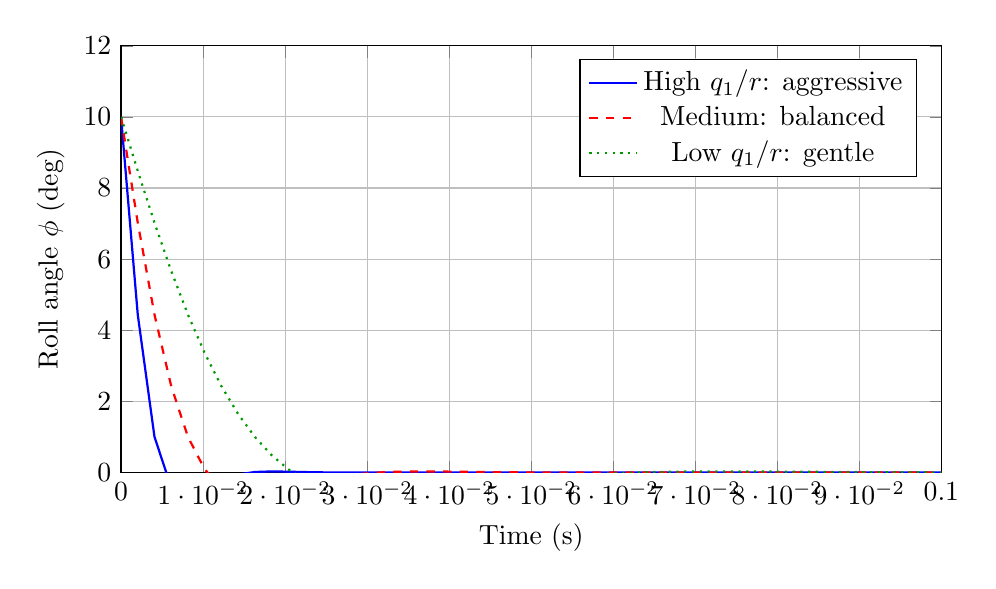
\begin{tikzpicture}
\begin{axis}[
    width=12cm, height=7cm,
    xlabel={Time (s)},
    ylabel={Roll angle $\phi$ (deg)},
    xmin=0, xmax=0.1,
    ymin=0, ymax=12,
    grid=major,
    legend pos=north east,
]
% High q1 (aggressive)
\addplot[blue, thick, domain=0:0.1, samples=50]
    {10*exp(-300*x)*cos(300*x*180/3.14159)};
\addlegendentry{High $q_1/r$: aggressive}

% Medium (balanced)
\addplot[red, thick, dashed, domain=0:0.1, samples=50]
    {10*exp(-150*x)*cos(150*x*180/3.14159)};
\addlegendentry{Medium: balanced}

% Low q1 (gentle)
\addplot[green!60!black, thick, dotted, domain=0:0.1, samples=50]
    {10*exp(-75*x)*cos(75*x*180/3.14159)};
\addlegendentry{Low $q_1/r$: gentle}

\end{axis}
\end{tikzpicture}
\end{center}

\begin{center}
\begin{tabular}{lccc}
\toprule
\textbf{Design} & $q_1/r$ & $\omega_n$ (rad/s) & Settling time (ms) \\
\midrule
Aggressive & $10^{-4}$ & 300 & 15 \\
Balanced & $10^{-5}$ & 150 & 30 \\
Gentle & $10^{-6}$ & 75 & 60 \\
\bottomrule
\end{tabular}
\end{center}

\textbf{Trade-off}: Higher $q_1/r$ gives faster response but requires more torque (larger gains), potentially causing motor saturation during aggressive maneuvers.

\section{LQR-Tuned PID: Bridging Theory and Practice}

While LQR provides optimal state feedback, practical implementations often use PID controllers for several reasons:
\begin{itemize}
    \item PID has integral action for steady-state error rejection
    \item PID operates on error, not absolute state
    \item PID is familiar to practitioners and easier to implement
\end{itemize}

The \textbf{LQR-tuned PID} approach combines the best of both worlds.

\subsection{From LQR Gains to PD Gains}

For the roll subsystem, LQR gives:
\[
\tau_\phi = -K_\phi \phi - K_p p
\]

A PD controller (without setpoint) is:
\[
\tau_\phi = K_P (\phi_d - \phi) + K_D (p_d - p)
\]

For regulation ($\phi_d = 0$, $p_d = 0$), these are identical with:
\begin{equation}
K_P = K_\phi, \quad K_D = K_p
\label{eq:lqr-to-pd}
\end{equation}

\subsection{Adding Integral Action}

LQR on the basic system has no integral action, leading to steady-state error under constant disturbances (e.g., center-of-mass offset, wind).

\textbf{Solution 1: Augment the state.}

Add an integrator state $\xi = \int \phi \, dt$ to get the augmented system:
\[
\begin{bmatrix} \dot{\phi} \\ \dot{p} \\ \dot{\xi} \end{bmatrix} =
\begin{bmatrix} 0 & 1 & 0 \\ 0 & 0 & 0 \\ 1 & 0 & 0 \end{bmatrix}
\begin{bmatrix} \phi \\ p \\ \xi \end{bmatrix} +
\begin{bmatrix} 0 \\ 1/J_x \\ 0 \end{bmatrix} \tau_\phi
\]

Design LQR with $\mathbf{Q} = \text{diag}(q_1, q_2, q_3)$ where $q_3$ weights the integrator state. This yields gains $[K_\phi, K_p, K_\xi]$ corresponding to a PID controller.

\textbf{Solution 2: Add integral term heuristically.}

Start with LQR-computed $K_P$ and $K_D$, then add $K_I$ empirically:
\begin{itemize}
    \item Start small: $K_I = 0.01 \cdot K_P$
    \item Increase until steady-state error is eliminated
    \item Ensure integral doesn't cause oscillation
\end{itemize}

\begin{lstlisting}[language=C, caption=LQR-tuned PID implementation]
// LQR-computed gains (from MATLAB)
#define KP_ROLL  3.87e-3f   // From LQR K[0]
#define KD_ROLL  5.57e-3f   // From LQR K[1]
#define KI_ROLL  0.05e-3f   // Added empirically

typedef struct {
    float integral;
    float prev_error;
} PIDState;

float pid_roll(PIDState* state, float phi_d, float phi, float p, float dt) {
    float error = phi_d - phi;

    // Anti-windup: limit integral
    state->integral += error * dt;
    state->integral = clamp(state->integral, -0.5f, 0.5f);

    // PID output
    float tau = KP_ROLL * error
              + KI_ROLL * state->integral
              + KD_ROLL * (0.0f - p);  // Assume p_d = 0

    return tau;
}
\end{lstlisting}

\subsection{Design Workflow}

\begin{enumerate}
    \item \textbf{Model}: Extract linearized subsystem (A, B matrices)
    \item \textbf{Specify}: Choose Q, R based on acceptable errors and actuator limits
    \item \textbf{Solve}: Compute LQR gains using MATLAB's \texttt{lqr()} or Python's \texttt{scipy.linalg.solve\_continuous\_are()}
    \item \textbf{Convert}: Map LQR gains to PD gains via \eqref{eq:lqr-to-pd}
    \item \textbf{Augment}: Add integral gain empirically or via augmented LQR
    \item \textbf{Implement}: Deploy as standard PID
    \item \textbf{Validate}: Test on hardware, fine-tune if needed
\end{enumerate}

\section{Full-State LQR vs. Cascaded PID}

For completeness, we compare full-state LQR (using all 12 states) with the cascaded PID architecture.

\subsection{Full-State LQR Design}

Using the full linearized model from Section~\ref{sec:linearization}:

\begin{lstlisting}[language=Matlab]
% Full 12-state model (simplified, without drag)
A = zeros(12,12);
A(1:3, 7:9) = eye(3);           % dp/dt = v
A(4:6, 10:12) = eye(3);         % dTheta/dt = omega (small angle)
A(7,5) = -g; A(8,4) = g;        % dv/dt depends on attitude

B = zeros(12,4);
B(9,1) = -1/m;                  % vz from thrust
B(10,2) = 1/Jx;                 % p from tau_phi
B(11,3) = 1/Jy;                 % q from tau_theta
B(12,4) = 1/Jz;                 % r from tau_psi

% LQR design
Q = diag([10 10 10 100 100 10 1 1 1 1 1 1]);  % Penalize attitude more
R = diag([1e6 1e6 1e6 1e6]);

K = lqr(A, B, Q, R);  % 4x12 gain matrix
\end{lstlisting}

The resulting 4×12 gain matrix $\mathbf{K}$ provides direct mapping from all states to all inputs---no cascade structure.

\subsection{Comparison}

\begin{center}
\begin{tabular}{lcc}
\toprule
\textbf{Aspect} & \textbf{Cascaded PID} & \textbf{Full-State LQR} \\
\midrule
\textbf{Gains to tune/specify} & 12--16 (4 PIDs) & 16 ($\mathbf{Q}$, $\mathbf{R}$ diagonals) \\
\textbf{Decoupling} & Manual (by design) & Automatic (MIMO) \\
\textbf{Physical intuition} & High (each loop clear) & Low (coupled gains) \\
\textbf{Implementation} & Simple (4 PIDs) & Complex (matrix multiply) \\
\textbf{States needed} & Errors only & Full state vector \\
\textbf{Integral action} & Built-in & Requires augmentation \\
\textbf{Robustness} & Adjustable per loop & Guaranteed margins \\
\textbf{Performance} & Very good & Optimal (by construction) \\
\textbf{Aggressive maneuvers} & May need gain scheduling & Handles coupling naturally \\
\bottomrule
\end{tabular}
\end{center}

\begin{keyidea}[title=When to Use Each Approach]
\textbf{Cascaded PID} is preferred when:
\begin{itemize}
    \item Implementation must be simple (limited MCU resources)
    \item Physical intuition and independent tuning are important
    \item Flight envelope is primarily hover and gentle maneuvers
    \item Integral action is essential (wind, weight variations)
\end{itemize}

\textbf{Full-State LQR} is preferred when:
\begin{itemize}
    \item Aggressive maneuvers with significant axis coupling
    \item Full state is available (e.g., from EKF)
    \item Systematic, reproducible tuning is needed
    \item Formal performance/robustness guarantees required
\end{itemize}

For most quadrotor applications, \textbf{LQR-tuned cascaded PID} provides an excellent compromise: principled gain selection with practical implementation.
\end{keyidea}

\section{LQG: Combining Kalman Filter and LQR}
\label{sec:lqg}

Chapter~\ref{ch:kalman-filter} developed the Kalman filter for state estimation; this chapter developed LQR for state feedback control. The \textbf{Linear Quadratic Gaussian (LQG)} controller combines them.

\subsection{The Separation Principle}

\begin{theorem}[Separation Principle]
For linear systems with Gaussian noise, the optimal controller consists of:
\begin{enumerate}
    \item A \textbf{Kalman filter} that computes $\hat{\mathbf{x}}$ from measurements
    \item An \textbf{LQR controller} that computes $\mathbf{u} = -\mathbf{K}\hat{\mathbf{x}}$
\end{enumerate}
These can be designed \textbf{independently}: the optimal estimator gain doesn't depend on the control cost, and the optimal control gain doesn't depend on the noise statistics.
\end{theorem}

\textbf{Intuition}: The Kalman filter provides the best estimate $\hat{\mathbf{x}}$ of the true state. Given this estimate, the best thing to do is apply the optimal control law as if $\hat{\mathbf{x}}$ were the true state.

\subsection{LQG Structure}

\begin{center}
\begin{tikzpicture}[
    block/.style={draw, rectangle, minimum height=2.5em, minimum width=4em, align=center},
    sum/.style={draw, circle, minimum size=1.5em, inner sep=0pt},
    >=Stealth
]
    % Plant
    \node[block] (plant) at (0,0) {Plant\\$\dot{\mathbf{x}} = \mathbf{A}\mathbf{x} + \mathbf{B}\mathbf{u}$};

    % Kalman filter
    \node[block, fill=blue!10] (kf) at (0,-2.5) {Kalman Filter\\$\hat{\mathbf{x}}$};

    % LQR
    \node[block, fill=green!10] (lqr) at (-4,-2.5) {LQR\\$\mathbf{u} = -\mathbf{K}\hat{\mathbf{x}}$};

    % Signals
    \draw[->] (plant.east) -- ++(1.5,0) node[right] {$\mathbf{y}$} |- (kf.east);
    \draw[->] (kf.west) -- (lqr.east) node[midway, above] {$\hat{\mathbf{x}}$};
    \draw[->] (lqr.west) -- ++(-1,0) |- (plant.west) node[near start, left] {$\mathbf{u}$};

    % Noise
    \draw[->] (1,1) node[above] {$\mathbf{w}$ (process)} -- (plant.north -| 0.5,0);
    \draw[->] (2,-1) node[right] {$\mathbf{v}$ (measurement)} -- (1.5,-1) -- (1.5,-0.5);

    % Annotation
    \node[draw, dashed, fit=(kf)(lqr), inner sep=10pt, label=below:LQG Controller] {};
\end{tikzpicture}
\end{center}

\subsection{Design Procedure}

\begin{enumerate}
    \item \textbf{Model}: Specify $\mathbf{A}$, $\mathbf{B}$, $\mathbf{C}$ matrices
    \item \textbf{Kalman filter}: Choose $\mathbf{Q}_{\text{KF}}$ (process noise), $\mathbf{R}_{\text{KF}}$ (measurement noise)
    \item \textbf{LQR}: Choose $\mathbf{Q}_{\text{LQR}}$ (state cost), $\mathbf{R}_{\text{LQR}}$ (control cost)
    \item \textbf{Compute}: Solve two Riccati equations (one for KF, one for LQR)
    \item \textbf{Implement}: Run Kalman filter, apply LQR control law
\end{enumerate}

\begin{lstlisting}[language=Matlab, caption=LQG design in MATLAB]
% System model
A = [0 1; 0 0];  B = [0; 1/Jx];  C = [1 0];

% Kalman filter design (estimate roll from noisy measurement)
Qkf = 1e-4;   % Process noise (gyro integration drift)
Rkf = 0.01;   % Measurement noise (accelerometer)
[Kf, ~, ~] = lqe(A, eye(2), C, Qkf*eye(2), Rkf);

% LQR design (control based on estimated state)
Qlqr = diag([10, 1]);  % State cost
Rlqr = 1e5;            % Control cost
[Kr, ~, ~] = lqr(A, B, Qlqr, Rlqr);

% Combined LQG: use Kr with estimated state from Kalman filter
% u = -Kr * x_hat
\end{lstlisting}

\subsection{LQG for Quadrotor Attitude}

Combining the attitude EKF from Chapter~\ref{ch:kalman-filter} with attitude LQR from Section~\ref{sec:lqr-attitude}:

See Listing~\ref{lst:lqg-controller} (Appendix~\ref{app:code-listings}) for the complete LQG attitude controller implementation that combines EKF state estimation with LQR feedback control.

\section{Practical Considerations}

\subsection{Gain Scheduling}

The linearized model is valid only near hover. For aggressive maneuvers:
\begin{itemize}
    \item Large angles invalidate small-angle approximations
    \item Thrust significantly different from $mg$
    \item Aerodynamic effects become nonlinear
\end{itemize}

\textbf{Solution}: \textbf{Gain scheduling}---use different LQR gains for different operating regions:

\begin{lstlisting}[language=C]
void select_gains(float phi, float theta, float thrust_ratio) {
    if (fabsf(phi) < 0.2f && fabsf(theta) < 0.2f &&
        thrust_ratio > 0.7f && thrust_ratio < 1.3f) {
        // Near hover: use nominal gains
        K = K_hover;
    } else {
        // Aggressive: use more conservative gains
        K = K_aggressive;
    }
}
\end{lstlisting}

\subsection{Actuator Saturation}

LQR assumes unconstrained control. When motors saturate:
\begin{itemize}
    \item Computed torques cannot be achieved
    \item Closed-loop behavior differs from design
    \item Integrators (if present) wind up
\end{itemize}

\textbf{Solutions}:
\begin{enumerate}
    \item \textbf{Conservative design}: Choose $\mathbf{R}$ to keep control within limits
    \item \textbf{Anti-windup}: Limit integrator states when saturated
    \item \textbf{Control allocation}: Prioritize attitude over position when saturated
\end{enumerate}

\subsection{Robustness Margins}

A key advantage of LQR is guaranteed stability margins:

\begin{theorem}[LQR Robustness]
For single-input LQR with $\mathbf{R} = r > 0$, the closed-loop system has:
\begin{itemize}
    \item \textbf{Gain margin}: $[\frac{1}{2}, \infty)$ (can double the gain without instability)
    \item \textbf{Phase margin}: $\geq 60°$
\end{itemize}
\end{theorem}

This robustness is ``free''---it comes from the optimization, not explicit design.

\begin{warningbox}[title=LQG Does Not Inherit LQR Robustness]
While LQR alone has excellent robustness margins, the combined LQG controller (LQR + Kalman filter) does \textbf{not} guarantee these margins. The Kalman filter introduces phase lag that can reduce stability margins.

\textbf{Mitigation}: Design the Kalman filter to be faster than the control bandwidth, or use loop transfer recovery (LTR) techniques.
\end{warningbox}

\section{Chapter Summary}

This chapter introduced optimal control methods for quadrotor attitude and position control:

\begin{itemize}
    \item \textbf{LQR} provides a systematic method for computing state-feedback gains by minimizing a quadratic cost function

    \item The \textbf{Algebraic Riccati Equation} gives optimal gains in terms of the cost weights $\mathbf{Q}$ (state penalty) and $\mathbf{R}$ (control penalty)

    \item \textbf{LQR-tuned PID} combines principled gain selection with practical integral action and familiar implementation

    \item \textbf{LQG} combines the Kalman filter (Chapter~\ref{ch:kalman-filter}) with LQR via the separation principle

    \item For most quadrotor applications, \textbf{cascaded PID with LQR-tuned gains} provides an excellent balance of performance, simplicity, and robustness
\end{itemize}

\begin{center}
\begin{tabular}{lll}
\toprule
\textbf{Method} & \textbf{Advantages} & \textbf{Best For} \\
\midrule
Hand-tuned PID & Simple, intuitive & Prototyping, one-off designs \\
LQR-tuned PID & Systematic, principled & Production systems \\
Full-state LQR & Optimal, handles coupling & Aggressive flight \\
LQG & Optimal estimation + control & Sensor fusion + control \\
\bottomrule
\end{tabular}
\end{center}

%======================================================================
\chapter{Parameter Identification}
%======================================================================

The mathematical models developed in this module contain physical parameters that must be determined for each specific quadrotor. This chapter presents systematic methods for identifying these parameters from measurements.

\section{Parameters to Identify}

The quadrotor dynamics model requires the following parameters:

\begin{center}
\begin{tabular}{llcc}
\toprule
\textbf{Parameter} & \textbf{Description} & \textbf{Units} & \textbf{Typical Value} \\
\midrule
$m$ & Total mass & kg & 0.027 (Crazyflie) \\
$I_{xx}$ & Roll moment of inertia & kg$\cdot$m$^2$ & $1.4 \times 10^{-5}$ \\
$I_{yy}$ & Pitch moment of inertia & kg$\cdot$m$^2$ & $1.4 \times 10^{-5}$ \\
$I_{zz}$ & Yaw moment of inertia & kg$\cdot$m$^2$ & $2.2 \times 10^{-5}$ \\
$L$ & Arm length (center to motor) & m & 0.046 \\
$C_T$ & Thrust coefficient & -- & 0.005 \\
$C_Q$ & Torque coefficient & -- & 0.0003 \\
$K_m$ & Motor constant & N/(rad/s)$^2$ & $3.5 \times 10^{-8}$ \\
$\tau_m$ & Motor time constant & s & 0.05 \\
\bottomrule
\end{tabular}
\end{center}

\begin{keyidea}[title=Parameter Identification Philosophy]
Some parameters can be measured directly (mass, arm length). Others require indirect methods based on dynamic response. The key is to design experiments that isolate individual parameters.
\end{keyidea}

\section{Mass and Geometry}

\subsection{Mass Measurement}

Total mass is measured directly using a precision scale:

\begin{lstlisting}[language=C, caption=Recording mass for flight log]
// Record mass as metadata for flight log
typedef struct {
    float total_mass_kg;     // Measured with scale
    float battery_mass_kg;   // Separate battery measurement
    float payload_mass_kg;   // Additional payload if any
} MassData;

// Total mass changes with battery charge level (minimal but measurable)
// For Crazyflie: ~27g without battery, ~34g with battery
\end{lstlisting}

\begin{notebox}[title=Mass Variation]
For accurate control, account for mass variation during flight:
\begin{itemize}
    \item Battery discharge: typically 1--2\% mass loss over flight
    \item Payload changes: if carrying variable loads
    \item Temperature effects: negligible for most applications
\end{itemize}
\end{notebox}

\subsection{Arm Length Measurement}

The arm length $L$ is the perpendicular distance from the center of mass to each rotor axis. For symmetric X-configuration quadrotors:

\[
L = \frac{d}{\sqrt{2}}
\]

where $d$ is the motor-to-motor diagonal distance.

\textbf{Measurement procedure}:
\begin{enumerate}
    \item Measure diagonal distance $d$ between opposite motor centers
    \item For X-configuration: $L = d / \sqrt{2}$
    \item For +-configuration: $L = d / 2$
    \item Verify center of mass is at geometric center (hang test)
\end{enumerate}

\section{Moment of Inertia Identification}
\index{moment of inertia}

The moments of inertia\index{moment of inertia|textbf} ($I_{xx}$, $I_{yy}$, $I_{zz}$) determine how quickly the quadrotor can rotate. Several methods exist for measurement.

\subsection{Bifilar Pendulum Method}

The bifilar pendulum is a classic technique for measuring moments of inertia:

%----------------------------------------------------------------------
% FIGURE: Bifilar Pendulum Setup
%----------------------------------------------------------------------
% Description: Quadrotor suspended by two parallel strings.
%
% Show:
%   - Quadrotor hanging level from two vertical strings
%   - String separation distance 'b'
%   - String length 'l'
%   - Angular displacement theta when twisted
%
% Dimensions: Half column width, ~5cm height.
%----------------------------------------------------------------------

The quadrotor is suspended by two parallel strings of length $l$, separated by distance $b$. When twisted and released, it oscillates with period $T$:

\begin{equation}
I = \frac{m g b^2 T^2}{16 \pi^2 l}
\label{eq:bifilar}
\end{equation}

See Listing~\ref{lst:bifilar} (Appendix~\ref{app:code-listings}) for the MATLAB implementation of Equation~\eqref{eq:bifilar}, including example measurements for a Crazyflie quadrotor.

\subsection{CAD-Based Estimation}

For initial estimates, CAD software can calculate moments of inertia if a detailed model exists with accurate material densities.

\subsection{Dynamic Identification from Flight Data}

Moments of inertia can also be identified from flight data by analyzing angular acceleration response to known torques:

\begin{equation}
I_{xx} \dot{\omega}_x = \tau_x \quad \Rightarrow \quad I_{xx} = \frac{\tau_x}{\dot{\omega}_x}
\end{equation}

See Listing~\ref{lst:dynamic-inertia} (Appendix~\ref{app:code-listings}) for a MATLAB script that identifies moment of inertia from step response flight data by analyzing angular acceleration.

\section{Thrust and Torque Coefficients}

The propulsion parameters $C_T$ and $C_Q$ (or equivalently $k_f$ and $k_\tau$) relate motor speed to thrust and torque:

\begin{align}
T &= C_T \rho D^4 \omega^2 = k_f \omega^2 \\
Q &= C_Q \rho D^5 \omega^2 = k_\tau \omega^2
\end{align}

\subsection{Thrust Stand Measurement}

The most reliable method uses a thrust test stand:

See Listing~\ref{lst:thrust-coeff} (Appendix~\ref{app:code-listings}) for a MATLAB script that fits $T = k_f \omega^2$ to thrust stand measurements and plots the fit quality.

\subsection{Torque Coefficient from Motor Constant}

The torque coefficient relates to thrust coefficient through the propeller geometry. A common approximation:

\[
\frac{k_\tau}{k_f} = \frac{C_Q}{C_T} \cdot D \approx c \cdot D
\]

where $c \approx 0.01$ for typical quadrotor propellers.

Alternatively, measure reaction torque directly:

See Listing~\ref{lst:torque-coeff} (Appendix~\ref{app:code-listings}) for a MATLAB script that identifies the torque coefficient from reaction torque measurements.

\section{Motor Dynamics Identification}

Motors have first-order dynamics that limit how fast thrust can change:

\[
\tau_m \dot{\omega}_m + \omega_m = \omega_m^{\text{cmd}}
\]

\subsection{Step Response Method}

Apply a step command and measure the rise time:

See Listing~\ref{lst:motor-timeconstant} (Appendix~\ref{app:code-listings}) for a MATLAB script that identifies the motor time constant from step response data using both the 63.2\% rise time method and nonlinear curve fitting.

\section{System Identification from Flight Data}

For complete system identification, frequency-domain methods provide robust results.

\subsection{Frequency Sweep Testing}

Inject sinusoidal commands of varying frequency and measure response:

See Listing~\ref{lst:freq-sweep} (Appendix~\ref{app:code-listings}) for a MATLAB script that processes frequency sweep flight test data to produce an experimental Bode plot using cross-correlation to extract gain and phase.

\subsection{Grey-Box System Identification}

Use MATLAB's System Identification Toolbox to fit a model structure with physical parameters:

See Listing~\ref{lst:greybox} (Appendix~\ref{app:code-listings}) for a complete grey-box system identification example using MATLAB's System Identification Toolbox. The code defines a parameterized state-space model for roll dynamics and estimates physical parameters ($I_{xx}$, $k_f$, $L$, $\tau_m$) from flight data.

\section{Validation}

Parameter identification is only useful if the results are validated.

\subsection{Cross-Validation}

Test the identified model on data not used for identification:

See Listing~\ref{lst:model-validate} (Appendix~\ref{app:code-listings}) for a MATLAB script that performs cross-validation by splitting data into training and validation sets.

\subsection{Physical Reasonableness}

Check that identified parameters are physically reasonable:

See Listing~\ref{lst:param-check} (Appendix~\ref{app:code-listings}) for a MATLAB function that validates identified parameters against physical constraints (reasonable inertia scaling, hover RPM range, motor time constant bounds).

\begin{keyidea}[title=Parameter Identification Best Practices]
\begin{enumerate}
    \item \textbf{Start simple}: Measure mass and geometry directly before trying dynamic methods
    \item \textbf{Design informative experiments}: Step responses and frequency sweeps excite dynamics
    \item \textbf{Use multiple methods}: Cross-check bifilar pendulum with dynamic identification
    \item \textbf{Validate thoroughly}: Test on held-out data and check physical reasonableness
    \item \textbf{Document everything}: Record test conditions, battery level, temperature
    \item \textbf{Iterate}: Initial flight tests may require updated parameters
\end{enumerate}
\end{keyidea}

\begin{warningbox}[title=Common Identification Pitfalls]
\begin{itemize}
    \item \textbf{Noisy data}: Filter appropriately before differentiation
    \item \textbf{Saturation}: Motor commands near limits give nonlinear response
    \item \textbf{Coupling}: Pure axis tests difficult; cross-coupling affects results
    \item \textbf{Air effects}: Ground effect, propeller wash affect hover tests
    \item \textbf{Battery variation}: Thrust changes with battery voltage
\end{itemize}
\end{warningbox}

\section{Module Summary}

This module has developed the complete framework for quadrotor orientation estimation:

\begin{enumerate}
    \item \textbf{Coordinate Frames and Transformations}
    \begin{itemize}
        \item World and body frames; NED convention
        \item Rotation matrices and their properties
        \item Euler angles: intuitive but singular (gimbal lock)
        \item Quaternions: robust and efficient
    \end{itemize}

    \item \textbf{Inertial Sensors}
    \begin{itemize}
        \item Gyroscope: accurate rates, but drifts
        \item Accelerometer: absolute roll/pitch reference, noisy during motion
        \item Magnetometer: yaw reference, susceptible to disturbances
    \end{itemize}

    \item \textbf{Orientation Estimation}
    \begin{itemize}
        \item Complementary filter: fuses sensors by frequency
        \item Mahony filter: practical 3D implementation
        \item Key insight: trust gyro for fast changes, accelerometer for long-term
    \end{itemize}

    \item \textbf{Quadrotor Dynamics}
    \begin{itemize}
        \item Forces and torques from motors
        \item Control allocation (mixing matrix)
        \item 12-state nonlinear model
        \item Linearization reveals cascaded control structure
    \end{itemize}
\end{enumerate}

In subsequent modules, you will implement these concepts on real hardware and design controllers for attitude and position regulation.
